\documentclass[11pt,twoside,a4paper,openright]{report}
%%%%%%%%%%%%%%%%%%%%%%%%%%%%%%%%%%%%%%%%%%%%%%%%
% Language, Encoding and Fonts
% http://en.wikibooks.org/wiki/LaTeX/Internationalization
%%%%%%%%%%%%%%%%%%%%%%%%%%%%%%%%%%%%%%%%%%%%%%%%
% Select encoding of your inputs. Depends on
% your operating system and its default input
% encoding. Typically, you should use
%   Linux  : utf8 (most modern Linux distributions)
%            latin1 
%   Windows: ansinew
%            latin1 (works in most cases)
%   Mac    : applemac
% Notice that you can manually change the input
% encoding of your files by selecting "save as"
% an select the desired input encoding. 
\usepackage[utf8]{inputenc}
% Make latex understand and use the typographic
% rules of the language used in the document.
\usepackage[danish,english]{babel}
% Use the palatino font
\usepackage[sc]{mathpazo}
\linespread{1.05}         % Palatino needs more leading (space between lines)
% Choose the font encoding
\usepackage[T1]{fontenc}

%%%%%%%%%%%%%%%%%%%%%%%%%%%%%%%%%%%%%%%%%%%%%%%%
% Graphics and Tables
% http://en.wikibooks.org/wiki/LaTeX/Importing_Graphics
% http://en.wikibooks.org/wiki/LaTeX/Tables
% http://en.wikibooks.org/wiki/LaTeX/Colors
%%%%%%%%%%%%%%%%%%%%%%%%%%%%%%%%%%%%%%%%%%%%%%%%
% load a colour package
\usepackage{xcolor}
\definecolor{aaublue}{RGB}{33,26,82}% dark blue

\definecolor{codegreen}{rgb}{0,0.6,0}
\definecolor{codegray}{rgb}{0.5,0.5,0.5}
\definecolor{codepurple}{rgb}{0.58,0,0.82}
\definecolor{backcolour}{rgb}{0.96,0.96,0.96}
\definecolor{backcolour}{rgb}{0.96,0.96,0.96}
\definecolor{newyellow}{rgb}{1,1,0.72}

% The standard graphics inclusion package
\usepackage{graphicx}
% Set up how figure and table captions are displayed
\usepackage{caption}
\captionsetup{%
  font=footnotesize,% set font size to footnotesize
  labelfont=bf % bold label (e.g., Figure 3.2) font
}
% Make the standard latex tables look so much better
\usepackage{array,booktabs}
% Enable the use of frames around, e.g., theorems
% The framed package is used in the example environment
\usepackage{framed}

% Adds support for full page background picture
\usepackage[contents={},color=gray]{background}
%\usepackage[contents=draft,color=gray]{background}

%%%%%%%%%%%%%%%%%%%%%%%%%%%%%%%%%%%%%%%%%%%%%%%%
% Mathematics
% http://en.wikibooks.org/wiki/LaTeX/Mathematics
%%%%%%%%%%%%%%%%%%%%%%%%%%%%%%%%%%%%%%%%%%%%%%%%
% Defines new environments such as equation,
% align and split 
\usepackage{amsmath}
% Adds new math symbols
\usepackage{amssymb}
% Use theorems in your document
% The ntheorem package is also used for the example environment
% When using thmmarks, amsmath must be an option as well. Otherwise \eqref doesn't work anymore.
\usepackage[framed,amsmath,thmmarks]{ntheorem}

%%%%%%%%%%%%%%%%%%%%%%%%%%%%%%%%%%%%%%%%%%%%%%%%
% Page Layout
% http://en.wikibooks.org/wiki/LaTeX/Page_Layout
%%%%%%%%%%%%%%%%%%%%%%%%%%%%%%%%%%%%%%%%%%%%%%%%
% Change margins, papersize, etc of the document
\usepackage[
  inner=28mm,% left margin on an odd page
  outer=41mm,% right margin on an odd page
  ]{geometry}
% Modify how \chapter, \section, etc. look
% The titlesec package is very configureable
\usepackage{titlesec}
\titleformat{\chapter}[display]{\normalfont\huge\bfseries}{\chaptertitlename\ \thechapter}{20pt}{\Huge}
\titleformat*{\section}{\normalfont\Large\bfseries}
\titleformat*{\subsection}{\normalfont\large\bfseries}
\titleformat*{\subsubsection}{\normalfont\normalsize\bfseries}
%\titleformat*{\paragraph}{\normalfont\normalsize\bfseries}
%\titleformat*{\subparagraph}{\normalfont\normalsize\bfseries}

% Clear empty pages between chapters
\let\origdoublepage\cleardoublepage
\newcommand{\clearemptydoublepage}{%
  \clearpage
  {\pagestyle{empty}\origdoublepage}%
}
\let\cleardoublepage\clearemptydoublepage

% Change the headers and footers
\usepackage{fancyhdr}
\pagestyle{fancy}
\fancyhf{} %delete everything
\renewcommand{\headrulewidth}{0pt} %remove the horizontal line in the header
\fancyhead[RE]{\small\nouppercase\leftmark} %even page - chapter title
\fancyhead[LO]{\small\nouppercase\rightmark} %uneven page - section title
\fancyhead[LE,RO]{\thepage} %page number on all pages
% Do not stretch the content of a page. Instead,
% insert white space at the bottom of the page
\raggedbottom
% Enable arithmetics with length. Useful when
% typesetting the layout.
\usepackage{calc}

%%%%%%%%%%%%%%%%%%%%%%%%%%%%%%%%%%%%%%%%%%%%%%%%
% Bibliography
% http://en.wikibooks.org/wiki/LaTeX/Bibliography_Management
%%%%%%%%%%%%%%%%%%%%%%%%%%%%%%%%%%%%%%%%%%%%%%%%
\usepackage[backend=bibtex,
  bibencoding=utf8,
  style=numeric-comp
  ]{biblatex}
\addbibresource{bib/mybib}

%%%%%%%%%%%%%%%%%%%%%%%%%%%%%%%%%%%%%%%%%%%%%%%%
% Misc
%%%%%%%%%%%%%%%%%%%%%%%%%%%%%%%%%%%%%%%%%%%%%%%%
% Add bibliography and index to the table of
% contents
\usepackage[nottoc]{tocbibind}
% Add the command \pageref{LastPage} which refers to the
% page number of the last page
\usepackage{lastpage}
% Add todo notes in the margin of the document
\usepackage[
%  disable, %turn off todonotes
  colorinlistoftodos, %enable a coloured square in the list of todos
  textwidth=\marginparwidth, %set the width of the todonotes
  textsize=scriptsize, %size of the text in the todonotes
  ]{todonotes}
%%%%%%%%%%%%%%%%%%%%%%%%%%%%%%%%%%%%%%%%%%%%%%%
%
% Package inserted by Emil Hammer 
%
%%%%%%%%%%%%%%%%%%%%%%%%%%%%%%%%%%%%%%%%%%%%%%%
 
\usepackage{enumitem}
\usepackage{listings}
\usepackage{amssymb}
\usepackage{nomencl}
\usepackage{siunitx}
\usepackage{hyperref}
\usepackage{etoolbox}

\usepackage{minted}



% Delete this if you want black/white code.
\lstdefinestyle{mystyle}{
    backgroundcolor=\color{backcolour},   
    commentstyle=\color{codegreen},
    keywordstyle=\color{magenta},
    numberstyle=\tiny\color{codegray},
    stringstyle=\color{codepurple},
    basicstyle=\ttfamily\footnotesize,
    breakatwhitespace=false,         
    breaklines=true,                 
    captionpos=b,                    
    keepspaces=true,                 
    numbers=left,                    
    numbersep=5pt,                  
    showspaces=false,                
    showstringspaces=false,
    showtabs=false,                  
    tabsize=2
}
\lstset{style=mystyle}

%%%%%%%%%%%%%%%%%%%%%%%%%%%%%%%%%%%%%%%%%%%%%%%%
% Hyperlinks
% http://en.wikibooks.org/wiki/LaTeX/Hyperlinks
%%%%%%%%%%%%%%%%%%%%%%%%%%%%%%%%%%%%%%%%%%%%%%%%
% Enable hyperlinks and insert info into the pdf
% file. Hypperref should be loaded as one of the 
% last packages
\usepackage{hyperref}
\hypersetup{%
	pdfpagelabels=true,%
	plainpages=false,%
	pdfauthor={Author(s)},%
	pdftitle={Title},%
	pdfsubject={Subject},%
	bookmarksnumbered=true,%
	colorlinks=false,%
	citecolor=black,%
	filecolor=black,%
	linkcolor=black,% you should probably change this to black before printing
	urlcolor=black,%
	pdfstartview=FitH%
    urlcolor=blue,
}



% package inclusion and set up of the document
% see, e.g., http://en.wikibooks.org/wiki/LaTeX/Formatting#Hyphenation
% for more information on word hyphenation
\hyphenation{ex-am-ple hy-phen-a-tion short}
\hyphenation{long la-tex}
% 
% see, e.g., http://en.wikibooks.org/wiki/LaTeX/Customizing_LaTeX#New_commands
% for more information on how to create macros

%%%%%%%%%%%%%%%%%%%%%%%%%%%%%%%%%%%%%%%%%%%%%%%%
% Macros for the titlepage
%%%%%%%%%%%%%%%%%%%%%%%%%%%%%%%%%%%%%%%%%%%%%%%%
%Creates the aau titlepage
\newcommand{\aautitlepage}[3]{%
  {
    %set up various length
    \ifx\titlepageleftcolumnwidth\undefined
      \newlength{\titlepageleftcolumnwidth}
      \newlength{\titlepagerightcolumnwidth}
    \fi
    \setlength{\titlepageleftcolumnwidth}{0.5\textwidth-\tabcolsep}
    \setlength{\titlepagerightcolumnwidth}{\textwidth-2\tabcolsep-\titlepageleftcolumnwidth}
    %create title page
    \thispagestyle{empty}
    \noindent%
    \begin{tabular}{@{}ll@{}}
      \parbox{\titlepageleftcolumnwidth}{
        \iflanguage{danish}{%
          
\includegraphics[width=\titlepageleftcolumnwidth]{AAUgraphics/aau_logo_da}
        }{%
          
\includegraphics[width=\titlepageleftcolumnwidth]{AAUgraphics/aau_logo_en}
        }
      } &
      \parbox{\titlepagerightcolumnwidth}{\raggedleft\sf\small
        #2
      }\bigskip\\
       #1 &
      \parbox[t]{\titlepagerightcolumnwidth}{%
      \textbf{Abstract:}\bigskip\par
        \fbox{\parbox{\titlepagerightcolumnwidth-2\fboxsep-2\fboxrule}{%
          #3
        }}
      }\\
    \end{tabular}
    \vfill
    \iflanguage{danish}{%
      \noindent{\footnotesize\emph{Rapportens indhold er frit tilgængeligt, men offentliggørelse (med kildeangivelse) må kun ske efter aftale med forfatterne.}}
    }{%
      \noindent{\footnotesize\emph{The content of this report is freely available, but publication (with reference) may only be pursued due to agreement with the author.}}
    }
    \clearpage
  }
}

%Create english project info
\newcommand{\englishprojectinfo}[8]{%
  \parbox[t]{\titlepageleftcolumnwidth}{
    \textbf{Title:}\\ #1\bigskip\par
    \textbf{Theme:}\\ #2\bigskip\par
    \textbf{Project Period:}\\ #3\bigskip\par
%    \textbf{Project Group:}\\ #4\bigskip\par
    \textbf{Participant:}\\ #5\bigskip\par
    \textbf{Supervisor:}\\ #6\bigskip\par
    \textbf{Copies:} #7\bigskip\par
    \textbf{Page Numbers:} \pageref{LastPage}\bigskip\par
    \textbf{Date of Completion:}\\ #8
  }
}

%Create danish project info
\newcommand{\danishprojectinfo}[8]{%
  \parbox[t]{\titlepageleftcolumnwidth}{
    \textbf{Titel:}\\ #1\bigskip\par
    \textbf{Tema:}\\ #2\bigskip\par
    \textbf{Projektperiode:}\\ #3\bigskip\par
    \textbf{Projektgruppe:}\\ #4\bigskip\par
    \textbf{Deltager(e):}\\ #5\bigskip\par
    \textbf{Vejleder(e):}\\ #6\bigskip\par
    \textbf{Oplagstal:} #7\bigskip\par
    \textbf{Sidetal:} \pageref{LastPage}\bigskip\par
    \textbf{Afleveringsdato:}\\ #8
  }
}

%%%%%%%%%%%%%%%%%%%%%%%%%%%%%%%%%%%%%%%%%%%%%%%%
% An example environment
%%%%%%%%%%%%%%%%%%%%%%%%%%%%%%%%%%%%%%%%%%%%%%%%
\theoremheaderfont{\normalfont\bfseries}
\theorembodyfont{\normalfont}
\theoremstyle{break}
\def\theoremframecommand{{\color{gray!50}\vrule width 5pt \hspace{5pt}}}
\newshadedtheorem{exa}{Example}[chapter]
\newenvironment{example}[1]{%
		\begin{exa}[#1]
}{%
		\end{exa}
}
% my new macros

\begin{document}
%frontmatter
\pagestyle{empty} %disable headers and footers
\pagenumbering{roman} %use roman page numbering in the frontmatter
\pdfbookmark[0]{Front page}{label:frontpage}%

\begin{titlepage}
\newgeometry{top=0cm,bottom=1.2cm,right=0cm,left=0cm}

  \backgroundsetup{
   scale=1.1,
   angle=0,
   opacity=1.0,  %% adjust
   contents={\includegraphics[width=\paperwidth,height=\paperheight]{AAUgraphics/aau_waves}}
    }
		
  \begin{center} %%please do not change the height or width of the frontpage image
    \centerline{
\includegraphics[totalheight=0.5\paperwidth,width=1\paperwidth]{AAUgraphics/frontpageImage}}% 
  \end{center}
	
	\vspace*{-0.96cm}
  {\noindent\color{aaublue}\fboxsep0pt\colorbox{white}{\begin{tabular}{@{}p{\paperwidth}@{}}
    \centerline{
    \begin{minipage}{0.85\textwidth}
        \bigskip
				\bigskip
        \centering
        \Huge{\textbf{
Internship at CERN % insert your title here
        }}
    \end{minipage}
    }
		
	\centerline{
	\begin{minipage}{0.9\textwidth}
        \bigskip
        \centering
        \Large{
Development of the EMP % insert your subtitle here
        }
    \end{minipage}
    }
			
	\centerline{
	\begin{minipage}{0.9\textwidth}
        \bigskip
        \centering
        {\Large
Emil Hammer Sandgaard% insert names separated by comma
        }
    \end{minipage}
    }
			
    \centerline{
    \begin{minipage}{0.9\textwidth}
        \bigskip
        \centering
        {\large
Electronic Engineering \the\year-06% insert name of study, group number, year-month
        } 
    \end{minipage}
    }
			
    \centerline{
    \begin{minipage}{0.9\textwidth}
        \bigskip
        \centering
%% Comment this section if you are not doing Bachelor or Master Project   
        {\Large
6. semester
      %Bachelor Project
        }
        \smallskip
    \end{minipage}
    }
			
  \end{tabular}}}

  \vfill
  \begin{figure}[!b]
	\centering
    
\includegraphics[width=0.2\paperwidth]{AAUgraphics/aau_logo_circle_en}% comment this line in for English version
    %\includegraphics[width=0.2\paperwidth]{AAUgraphics/aau_logo_circle_da} %comment this line in for Danish version
  \end{figure}
\end{titlepage}
\restoregeometry
\pdfbookmark[0]{Front page}{label:frontpage}%
\begin{titlepage}
\vspace*{\fill}
    \backgroundsetup{
    scale=1.1,
    angle=0,
    opacity=1.0,  %% adjust
    contents={\includegraphics[width=\paperwidth,height=\paperheight]{AAUgraphics/aau_waves}}
    }
  \addtolength{\hoffset}{0.5\evensidemargin-0.5\oddsidemargin} %set equal margins on the frontpage - remove this line if you want default margins
  \noindent%
  {\color{white}\fboxsep0pt\colorbox{aaublue}{\begin{tabular}{@{}p{\textwidth}@{}}
    \begin{center}
    \Huge{\textbf{
      Internship at CERN% insert your title here
    }}
    \end{center}
    \begin{center}
      \Large{
        Development of Something% insert your subtitle here
      }
    \end{center}
    \vspace{0.2cm}
   \begin{center}
    {\Large
      Emil Hammer Sandgaard% insert names separated by comma
    }\\
    \vspace{0.2cm}
    {\large
      Electronic Engineering% insert name of the study, group number, year-month
    }
   \end{center}
   \vspace{0.2cm}
%% Comment this section in if you are doing Bachelor or Master Project   
   \begin{center}
    {\Large
     Project
    } 
   \end{center}
  \end{tabular}}}
  \vfill
  \begin{center}
    
\includegraphics[width=0.2\paperwidth]{AAUgraphics/aau_logo_circle_en}% comment this line in for English version
    %\includegraphics[width=0.2\paperwidth]{AAUgraphics/aau_logo_circle_da} %comment this line in for Danish version
  \end{center}
\end{titlepage}
\clearpage

\thispagestyle{empty}
{\small
\strut\vfill % push the content to the bottom of the page
\noindent Copyright \copyright{} Aalborg University 2015\par
\vspace{0.2cm}
\noindent Here you can write something about which tools and software you have used for typesetting the document, running simulations and creating figures. If you do not know what to write, either leave this page blank or have a look at the colophon in some of your books.
}
\clearpage


\pdfbookmark[0]{English title page}{label:titlepage_en}
\aautitlepage{%
  \englishprojectinfo{
    Internship report  %title
  }{%
    Internship at CERN %theme
  }{%
    Spring Semester 2022 %project period
  }{%
    % Project group
  }{%
    %list of group members
    Emil Hammer Sandgaard\ 
  }{%
    %list of supervisors
    Vladimir Ryjov
  }{%
    1 % number of printed copies
  }{%
    \today % date of completion
  }%
}{%department and address
  \textbf{Electronics and IT} \\
  Aalborg University \\
  \href{http://www.aau.dk}{http://www.aau.dk}
}{% the abstract
This report is aimed to sum up my internship at CERN. 

Throughout this report, I will give insight into the work done during the period, with an introduction of the hardware used and a technical description of the development made. Furthermore, the report clarifies the knowledge and experience acquired at CERN in parallel with my education at Aalborg University in both a technical and environmental manner.  
Furthermore, the report will describe CERN, its achievement, and how the organization is formed.

The report will further discuss the advantages of working abroad and my personal experience. 
}

% \cleardoublepage
% {\selectlanguage{danish}
% \pdfbookmark[0]{Danish title page}{label:titlepage_da}
% \aautitlepage{%
%   \danishprojectinfo{
%     Rapportens titel %title
%   }{%
%     Semestertema %theme
%   }{%
%     Efterårssemestret 2010 %project period
%   }{%
%     XXX % project group
%   }{%
%     %list of group members
%     Forfatter 1\\ 
%     Forfatter 2\\
%     Forfatter 3
%   }{%
%     %list of supervisors
%     Vejleder 1\\
%     Vejleder 2
%   }{%
%     1 % number of printed copies
%   }{%
%     \today % date of completion
%   }%
% }{%department and address
%   \textbf{Elektronik og IT}\\
%   Aalborg Universitet\\
%   \href{http://www.aau.dk}{http://www.aau.dk}
% }{% the abstract
%   Her er resuméet
% }}
%\cleardoublepage
\pdfbookmark[0]{Contents}{label:contents}
\pagestyle{fancy} %enable headers and footers again //
\tableofcontents
\listoftodos
%\chapter*{Preface}
\addcontentsline{toc}{chapter}{Preface}

%  Denne rapport er udarbejdet under 3. semesters projektforløb i efteråret 2020 på Elektronik og IT uddannelsen, hvor studieordningen fokuserer på analoge kredsløb og systemer.
% \textbf{Læsevejledning}
%  I rapporten vil der fremtræde kildehenvisninger og en samlet kildeliste over disse kan findes bagerst i rapporten inden bilag og appendiks.
%  Kildehenvisningen er efter Vancouver-metoden, så i teksten refereres en kilde til på formen %\say{[Nr.]}, hvor kilderne er nummereret efter optrædende. Ligeledes er kildelisten nummereret efter optræden.
%  Hvis årstallet for udgivelsen var utilgængelig, vil kildelisten vise årstallet for besøgelse. 
%  Henvisningerne fører med hyperlinks ned til kildelisten, hvor kilder er angivet med forfatter, titel, evt. link, udgivelsesmåned, -år og dato for besøg.
%  Figurer, tabeller mm. er nummereret i forhold til hvilket kapitel de findes i, hvilket vil sige, at den første figur i kapitel to har nummer 2.1 og den næste har 2.2 osv. Forklarende tekst for figurer findes under de givne figurer, hvorimod den forklarende tekst til tabeller findes over. Efter kildelisten findes appendiksene og bilagene, der bliver nummeret med bogstaver.

%  Fodnoten bliver brugt som \textit{den forklarende/uddybende note}, hvori en forklaring af enkelte ord/forkortelser indgår.

%  Der benyttes videnskabelige præfikser og enheder i overensstemmelse med ISO-80000.
% % Der anvendes $\ca{E96}$, når der laves approksimationer til E96 modstandsrækken.

%\vspace{\baselineskip}\hfill Aalborg University, \today
\vfill\noindent

% \begin{minipage}[b]{0.45\textwidth}
%  \centering
%  \rule{\textwidth}{0.5pt}\\
%   Author 1\\
%  {\footnotesize <username1@XX.aau.dk>}
% \end{minipage}
% \hfill
% \begin{minipage}[b]{0.45\textwidth}
%  \centering
%  \rule{\textwidth}{0.5pt}\\
%   Author 2\\
%  {\footnotesize <username2@XX.aau.dk>}
% \end{minipage}


\vspace{3\baselineskip}
\begin{center}
\begin{minipage}[b]{0.5\textwidth}
\vspace{15cm}
 \centering
 \rule{\textwidth}{0.9pt}
  Emil Hammer Sandgaard\\
 {\footnotesize esandg18@student.aau.dk}\\
 {\footnotesize emil.hammer.sandgaard@cern.ch}
\end{minipage}
\end{center}

\makenomenclature
\addcontentsline{toc}{chapter}{Nomenclature}


%% This will add the subgroups
%----------------------------------------------
\renewcommand\nomgroup[1]{%
  \item[\bfseries
  \ifstrequal{#1}{A}{Physics Constants}{%
  \ifstrequal{#1}{B}{Hardware}{%
  \ifstrequal{#1}{C}{Other conventions}{}}}%
]}
%----------------------------------------------

%% This will add the units
%----------------------------------------------
\newcommand{\nomunit}[1]{%
\renewcommand{\nomentryend}{\hspace*{\fill}#1}}
%----------------------------------------------

% \nomenclature[B, 01]{For.}{{Udd.} \nomunit{\newline \textit{Besk}}}

%%%
\nomenclature[A, 01]{\(G\)}{{Gravitational constant} \nomunit{\newline \textit{Front-end counterpart to the EMP
housing an lpGBT.}}}
%%%
\nomenclature[B, 01]{VL+:}{{Versatile Link+} \nomunit{\newline \textit{Used for high speed optical links }}}
\nomenclature[B, 02]{EMP:}{{Embedded Monitoring Processor}\nomunit{\newline \textit{}} }
\nomenclature[B, 03]{EMCI:}{{Embedded 
Monitoring and Control Interface} \nomunit{\newline \textit{Front-end counterpart to the EMP
housing an lpGBT.}}}


\nomenclature[B, 04]{MPSoC:}{{Mulit purpose system-on-chip} \nomunit{\newline \textit{Includes programmable logic}}}

%%%
\nomenclature[C,01]{Ex}{Ex3}

\nomenclature[C, 01]{PL:}{{Programmerable Logic} \nomunit{\newline \textit{(FPGA)}}}
\nomenclature[C, 02]{PS: }{{Processing system} \nomunit{\newline \textit{Besk}}}
\printnomenclature

\chapter*{Prerequisites}
\addcontentsline{toc}{chapter}{Prerequisites}

This report is not targeting for learning - and should not either be considered as a manual. The reader must in that regard have a understanding for the following concepts introduced throughout this report to have a common ground.

\begin{itemize}
    \item Basic Linux knowledge 
    
\end{itemize}

\newpage
%\cleardoublepage
%mainmatter
\pagenumbering{arabic} %use arabic page numbering in the mainmatter 
\chapter{Introduction}

This chapter will begin with an introduction of CERN, followed by a description of the organization and its governance. Finally, the chapter will describe my personal experiences in that context.

\section{CERN}

European Organization for Nuclear Research, or CERN, was established in 1954 after world war II in a multilateral intergovernmental treaty. They research in particle physics with high-energy experiments, where CERN is most known for the Large Hadron Collider, or LHC, the world's largest particle collider. \\

\noindent CERN is placed at the French/Swiss border with the headquarters in Meyrin, Switzerland, near Geneva. In 2017, more than 17500 people from around the globe worked together at CERN, of which 2500 were CERN employees, and the rest were users of the facilities \cite{OurPeopl98:online}. Throughout the history of CERN, outstanding achievements and discoveries have been made. Among them is the significant discovery of the Higgs boson.\\ 

\noindent The establishment of CERN was made with the desire to bring nations together through science with four fundamental tasks:

\begin{itemize}
    \item \textbf{Research:} Seeking and finding answers about the universe
    \item \textbf{Technology:} Advancing the frontier of technology
    \item \textbf{Collaboration:} Bringing nations together through science
    \item \textbf{Education:} Training the scientists of tomorrow
\end{itemize}

\noindent These are the core values of CERN and are what the CERN council strives to achieve.\\

\noindent As CERN includes employees from all over the world. Diversity is undoubtedly a core feature of the people of CERN. At CERN, this diversity is utilized to create creativity and innovation between the diverse ideas, perspectives, and approaches unfolding between nations and differences. Bringing people together to share ideas and knowledge is ideal for learning and growth. 

\section{Organizational Structure}

At CERN, the organizational structure is hierarchical. At the top of the hierarchy lies the CERN council. This council is the highest authority of the organization of CERN and is composed of delegates of all twenty-three member states. They have the vital purpose of determining the scientific policy of the organization with respect to the treaty. This includes decisions regarding the budget, annual goals, etc. On figure \ref{fig:pic193} below, the structure hierarchy is shown.
\begin{figure}[H]
    \centering
    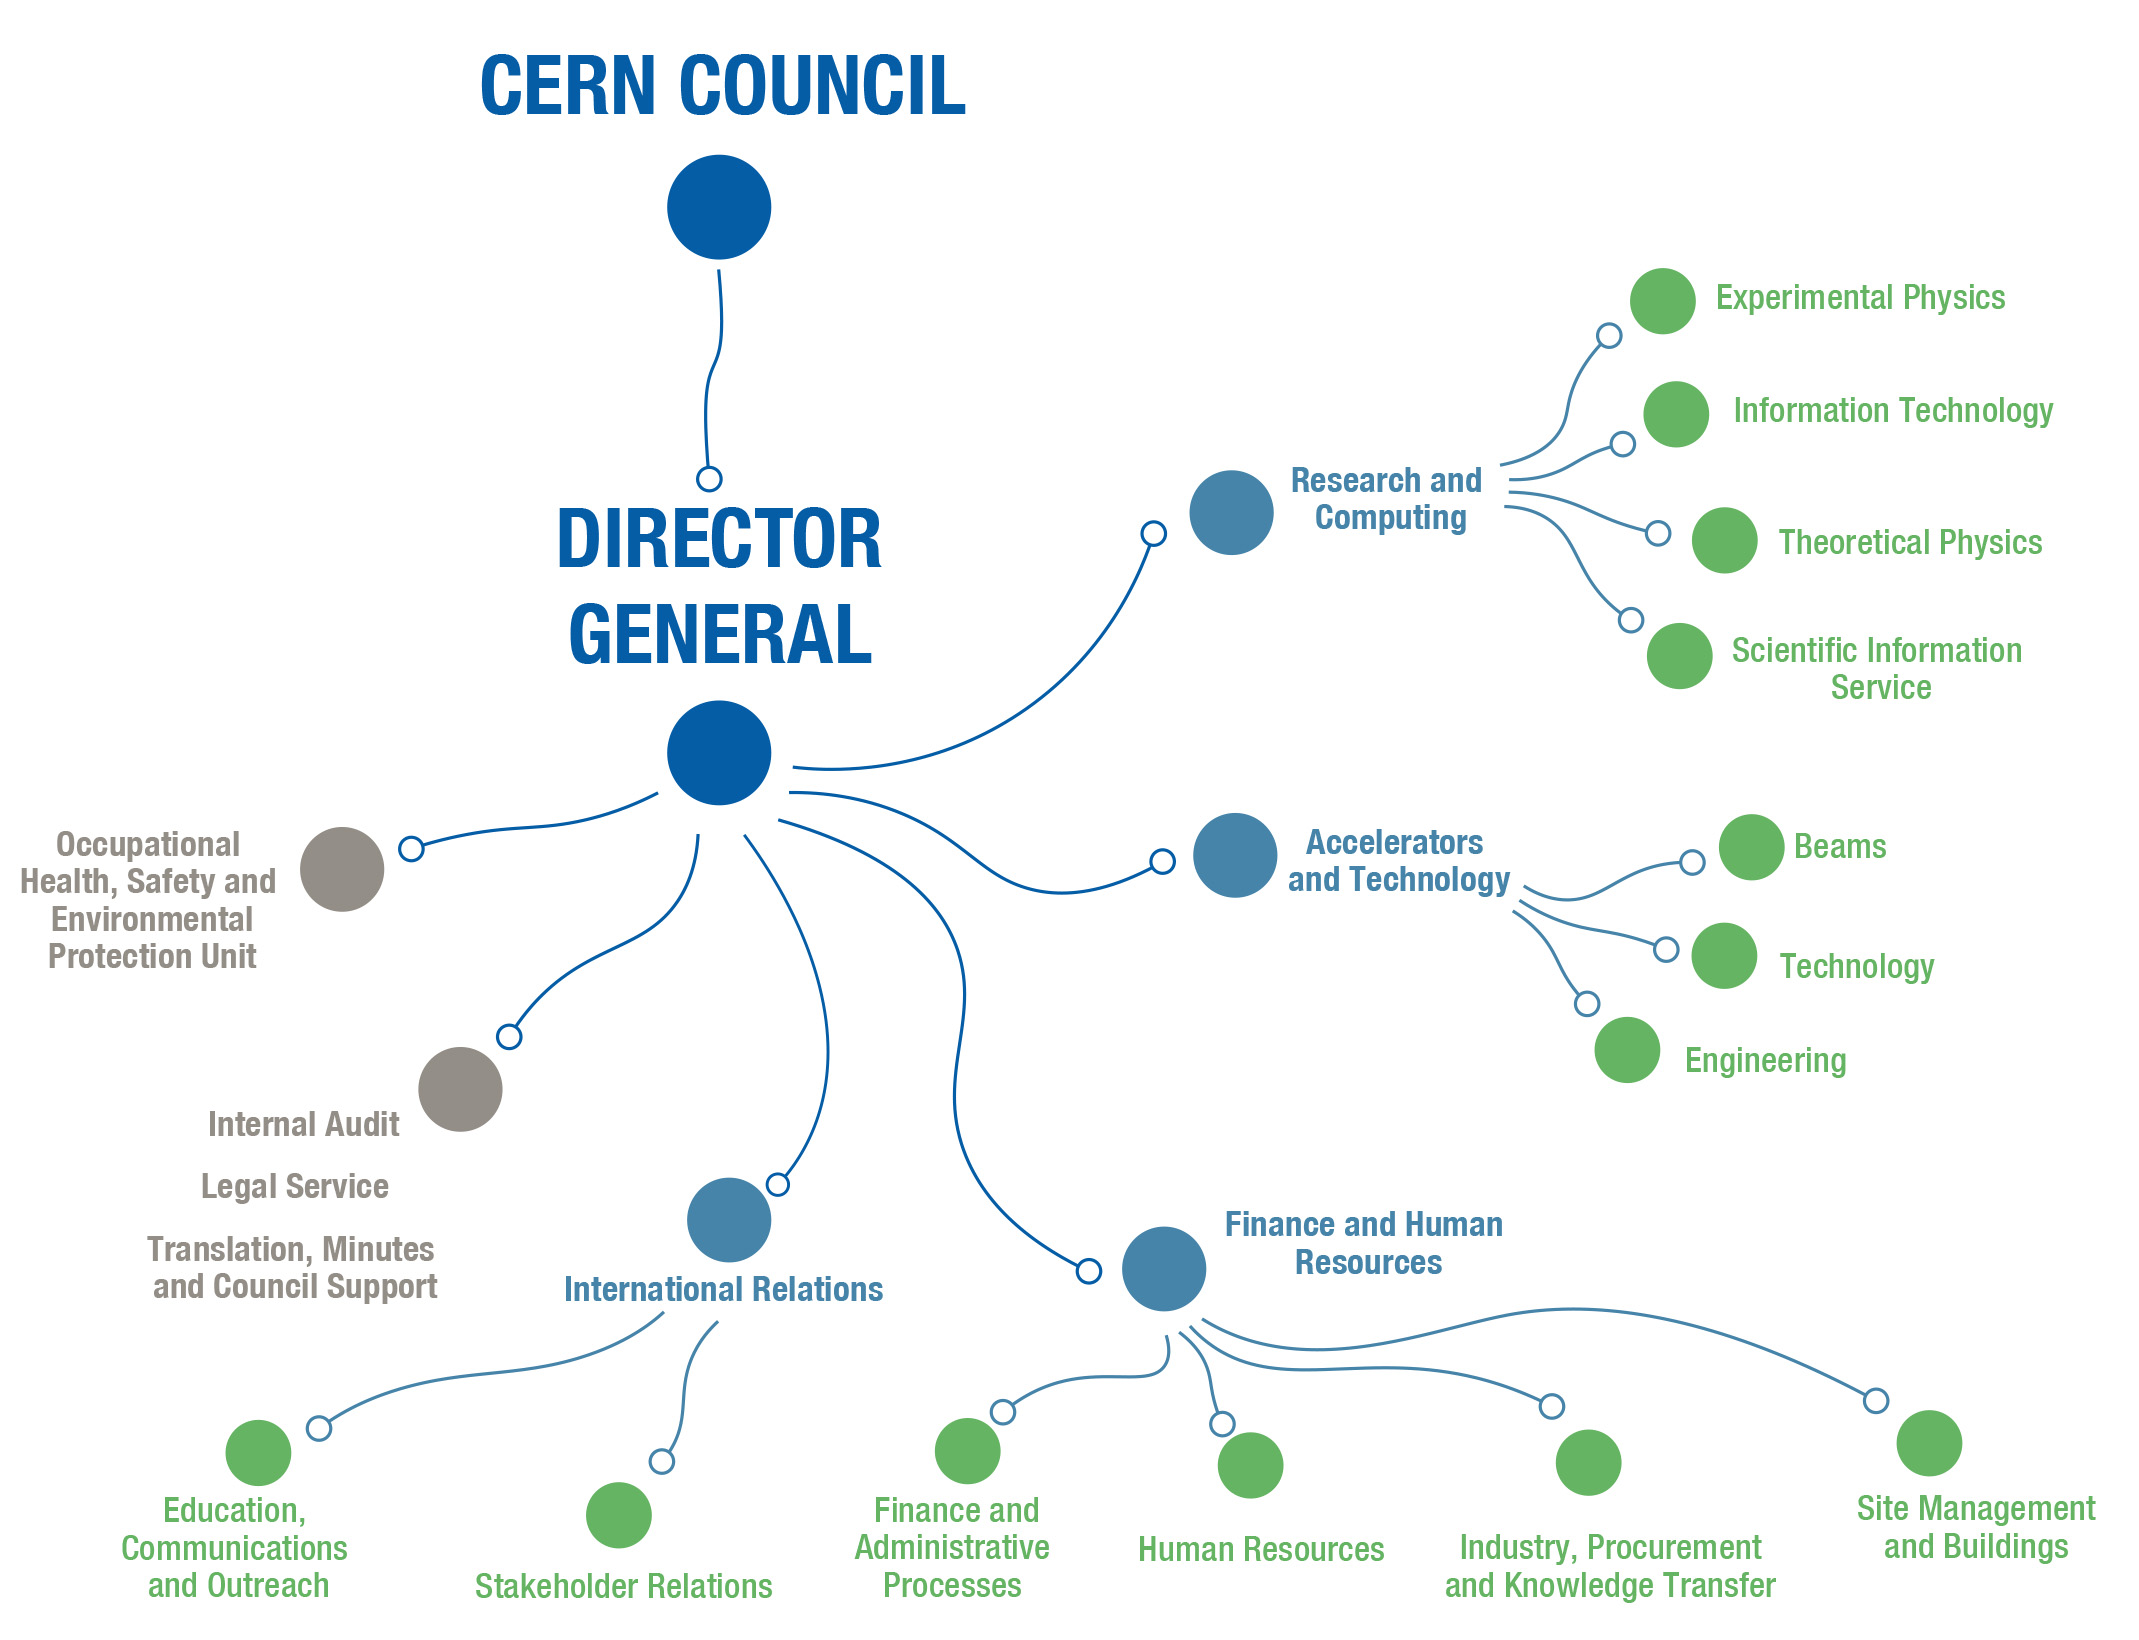
\includegraphics[width=1\textwidth]{AAUgraphics/AboutCERN_Organigramme.jpg}
    \caption{CERN organisation \cite{Environm54:online}.}
    \label{fig:pic193}
\end{figure}

\noindent Below the CERN council is the director-general, Fabiola Gianotti. She reports directly to the council and can propose adjustments considered necessary to meet the needs of the research programs. Below her, the hierarchy splits into six categories. 

\begin{itemize}
    \item International Relations Sector (IR)
    \item Research and Computing Sector (RCS)
    \item Accelerators and Technology Sector (ATS)
    \item Finance and Human Resources Sector (FHRS)
    \item Internal audit (DG)
    \item Occupational Health, Safety and Environmental Protection Unit (HSE)
\end{itemize}

\noindent During my internship, I was in the Experimental Physics (EP) department, which falls under the category RCS. The Experimental Physics department is furthermore split into eleven groups. Where I was in the Electronics Systems for Experiments (ESE) group, and which again, is split into three different sections. Where I was in the Front-End Systems (FE) section. To sum up, this means that in total, my group was EP-ESE-FE, which consists of the initials for Experimental Physics (EP), Electronics Systems for Experiments (ESE) and Front-End Systems (FE).\\

\noindent Even though the organization's architecture has this hierarchical structure. It does not feel that way when working. From my point of view, the team I worked in felt like its own little company with the freedom to operate towards the goal without interference from the above layers of the hierarchy. Also worth mentioning is that despite the size of CERN and all the layers in the hierarchy, it never felt overwhelming big, and the work was done in collaboration between different sections, so there was never a feeling of "us" and "them".\\

\noindent The team I worked in had three members: me, my supervisor Vladimir Ryjov (from Russia), and Daniel Blasco (from Spain). Unfortunately, Daniel left after three months due to a job offer he couldn't resist. So from that point, the team consisted of Vladimir and me. However, even though it was "just" Vladimir and me on the team, the project - which will be described later - was a collaborative effort with another small team from ATLAS.

% Unfortunately danish people are a minority at CERN. It's hard to get danish students to CERN because of the good conditions in Denmark. Derived from this problem CERN has established a Danish Student Program, to get more applicants from Denmark. 

\chapter{The Project}

During the internship, the primary purpose was to contribute to the ATLAS detector control system by supporting the development of the Embedded Monitoring processor, abbreviated as EMP. The EMP is a processing platform targeting for the experiments in the HL-LHC upgrade. It serves as an interface between up to 12 Embedded Monitoring Control Interfaces (EMCI) and the control room.

\begin{figure}[H]
    \centering
    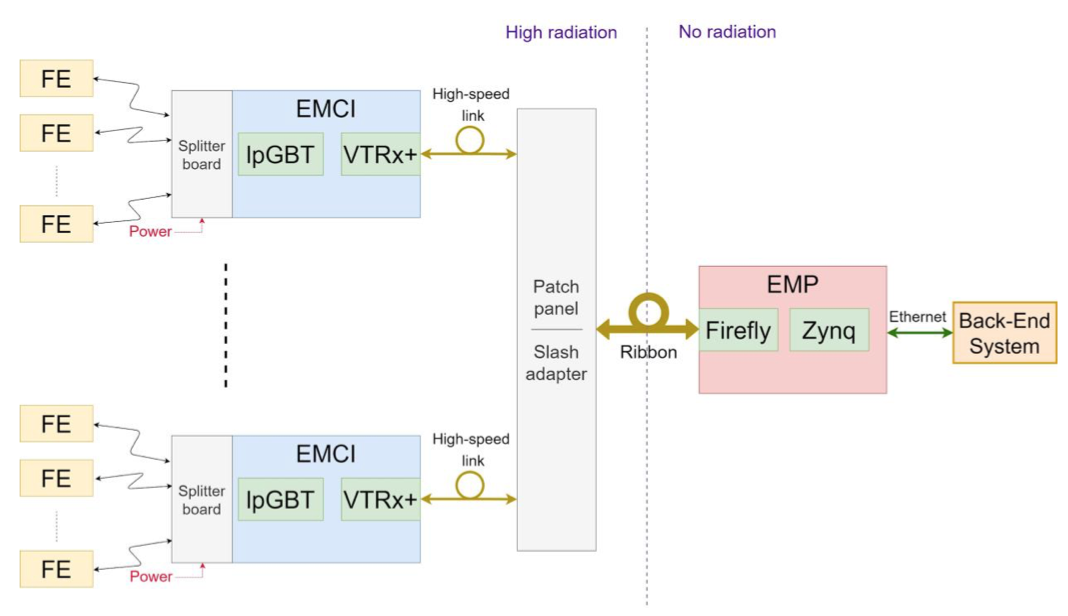
\includegraphics[width=1\textwidth]{Graphics/pic 1.png}
    \caption{The EMCI and EMP system.}
    \label{fig:pic1}
\end{figure}

\noindent In the figure \ref{fig:pic1} it can be seen how Front ends (FE) is sending data back to the EMCI. The EMCI receives this data and sends it back to the EMP through the VTRx+ optical link. Here it is worth mentioning that the EMP is placed in a non-radiation environment, which means that the components of the EMP can be built from COTS components. Opposite the EMP, the EMCI and FE are placed in a harsh radiation environment. This means that these components have to be carefully designed to withstand this radiation. \\

\section{Hardware introduction}

As the EMP is developed using multiple components and systems, this chapter will briefly introduce the relevant hardware mentioned throughout this report and give a walk-through of the setup.

\subsection{The "remote" PC}

As the EMP is limited in processing power, a PC is used to assist the development. This PC is referred to as the "remote" PC. The remote PC is, by choice, not connected to any screen, mouse, or keyboard and is instead used through Secure Shell or SSH. The SSH, combined with the Linux OS, allows collaboration to be more convenient, as several people easy can connect to it simultaneously. Further, it can be operated by just being connected to the internet. \\

\noindent The remote PC hosts the network file system or NFS, which is responsible for booting the EMP (which serves as the client). The NFS also means the remote PC can access all files on the EMP through NFS. The file system of the EMP is located in the path \textbf{/tftpboot/emp-01-00-02-centos8/} on the remote PC. The advantages of using NFS in this project include:

\begin{itemize}
    \item Move files between systems with ease
    \vspace{-0.2 cm}
    \item Modify files, folders, etc. on the EMP
    \vspace{-0.2 cm}
    \item Edit code present on the EMP, with the remote PC. Allowing software like VSC to be used. However, the code must still be compiled on EMP.
\end{itemize}

\noindent However, the NFS will most likely not be part of the final product, as the final product should be operating as a standalone product.

\begin{figure}[H]
     \centering
     \begin{subfigure}[b]{0.45\textwidth}
         \centering
         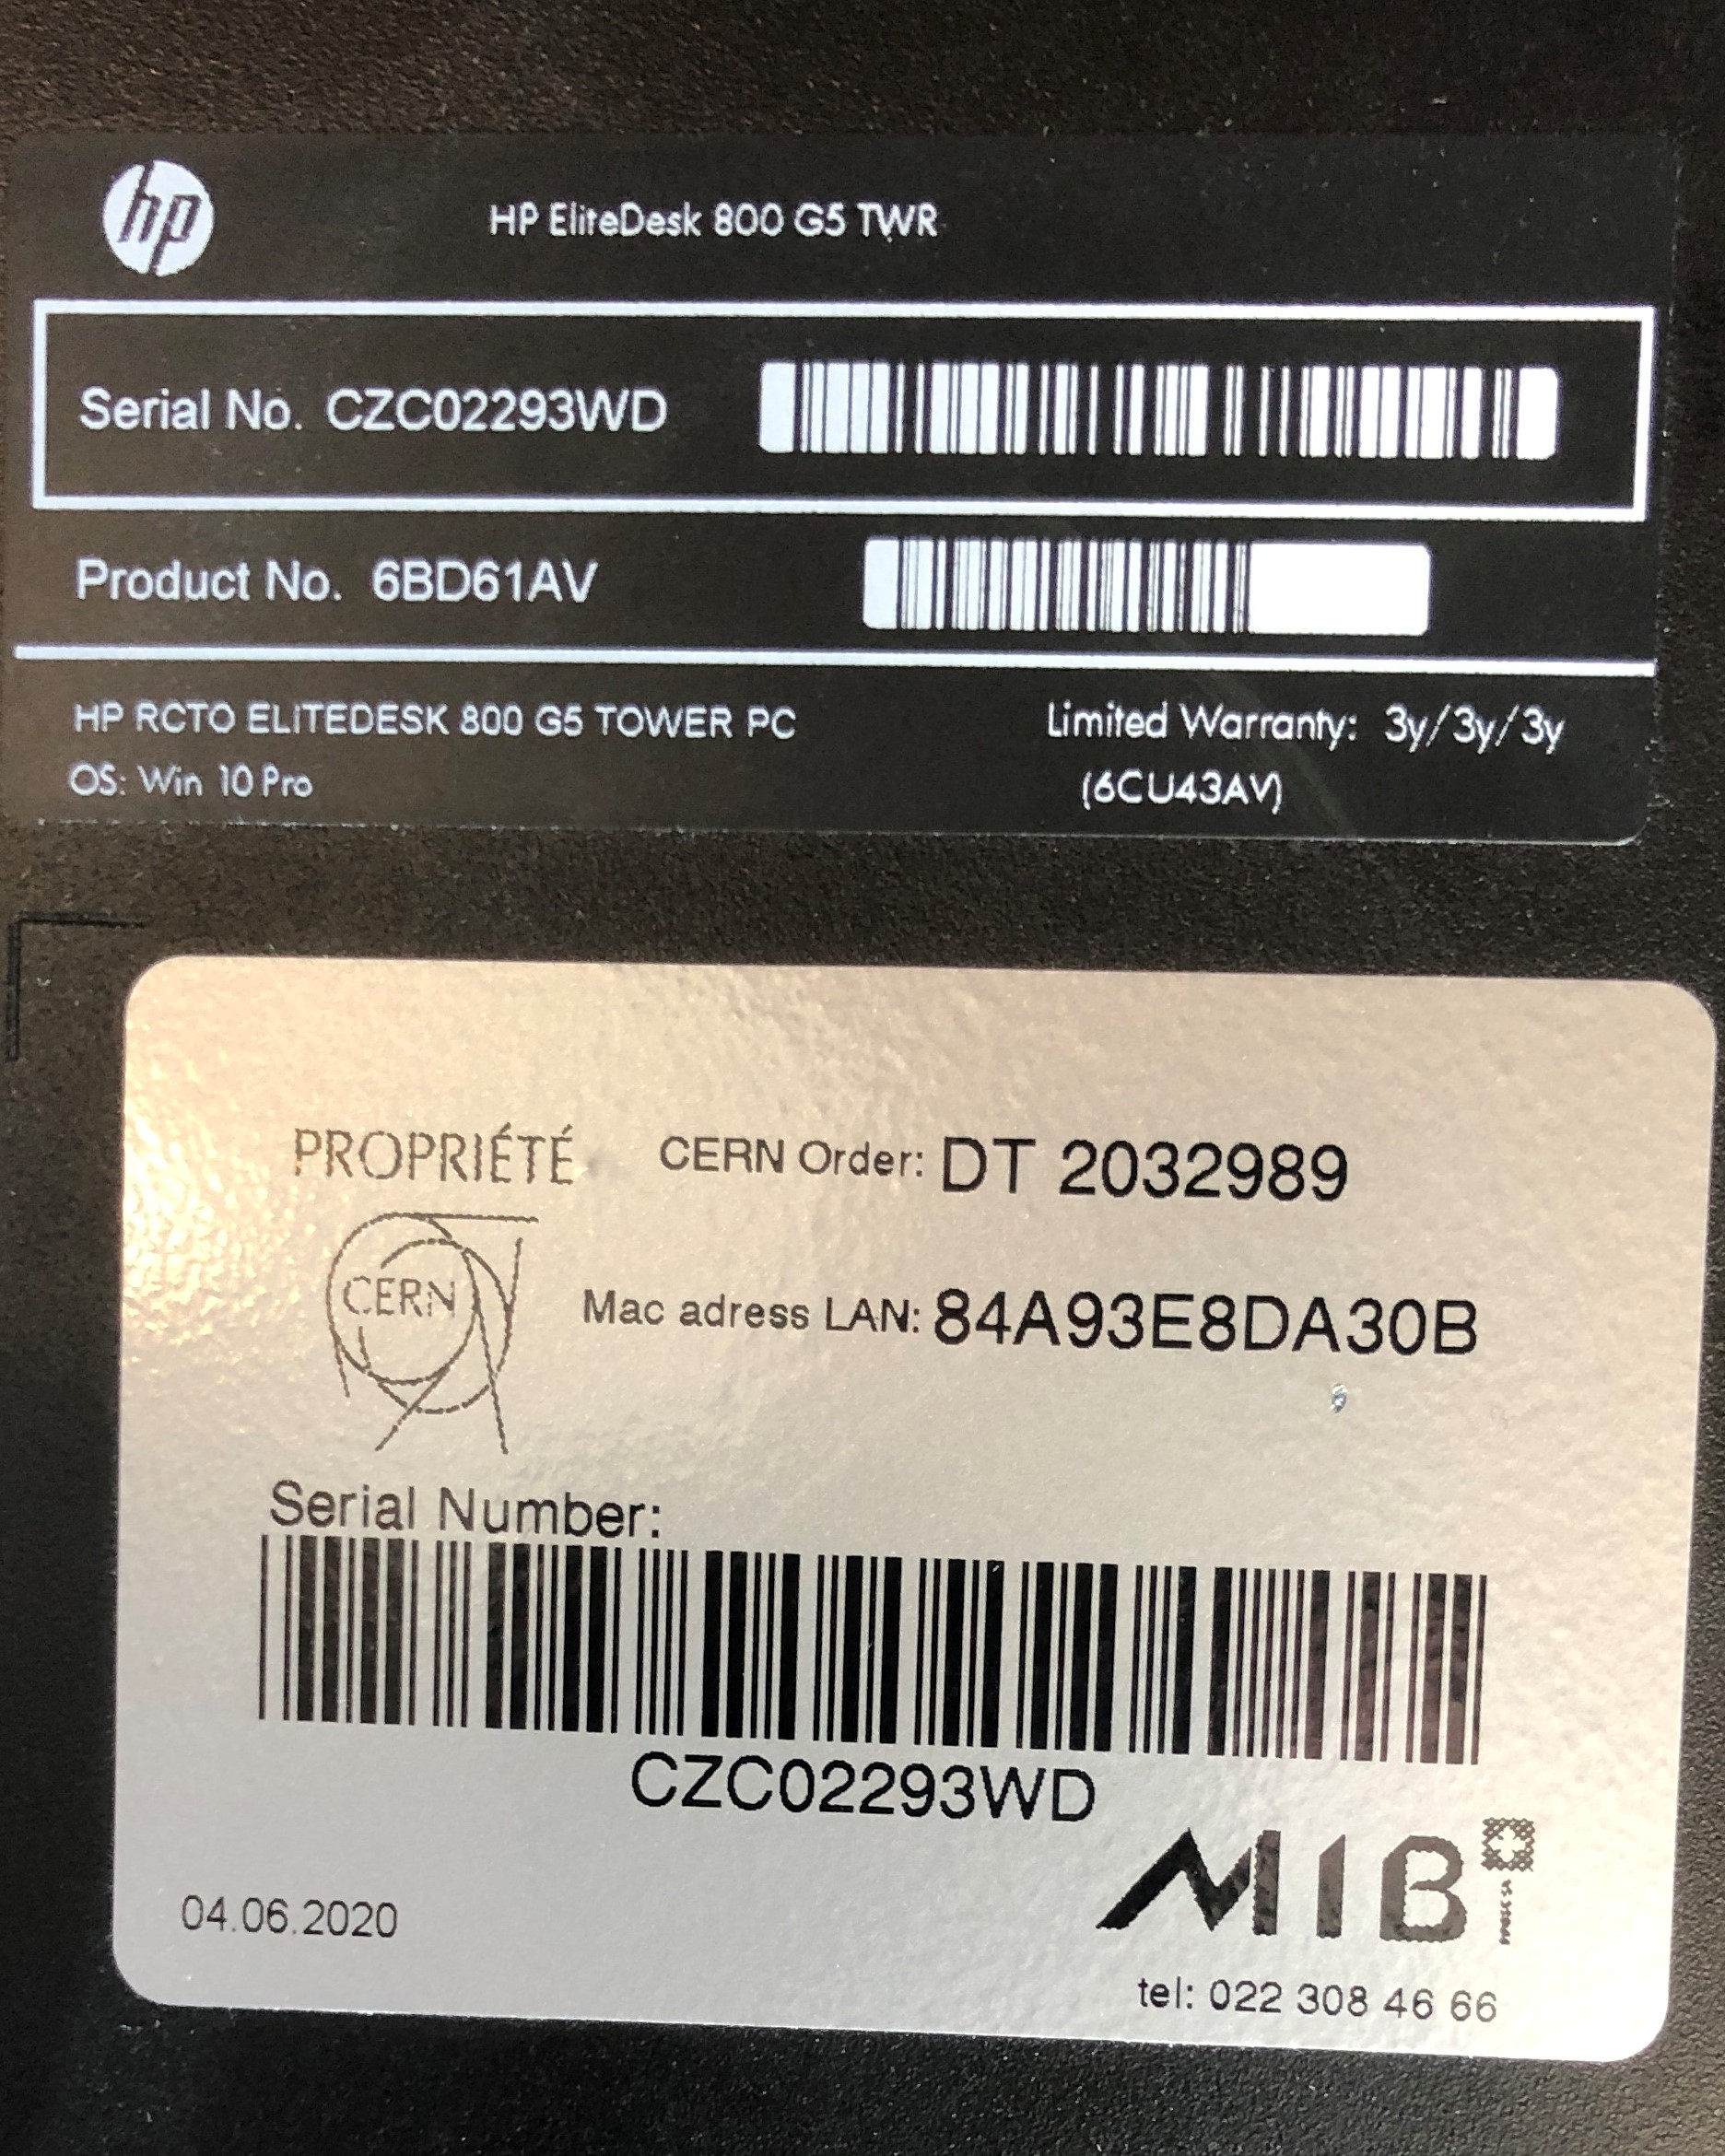
\includegraphics[width=1\textwidth]{Graphics/remPCtop.jpg}
     \end{subfigure}
     \hfill
     \begin{subfigure}[b]{0.45\textwidth}
         \centering
         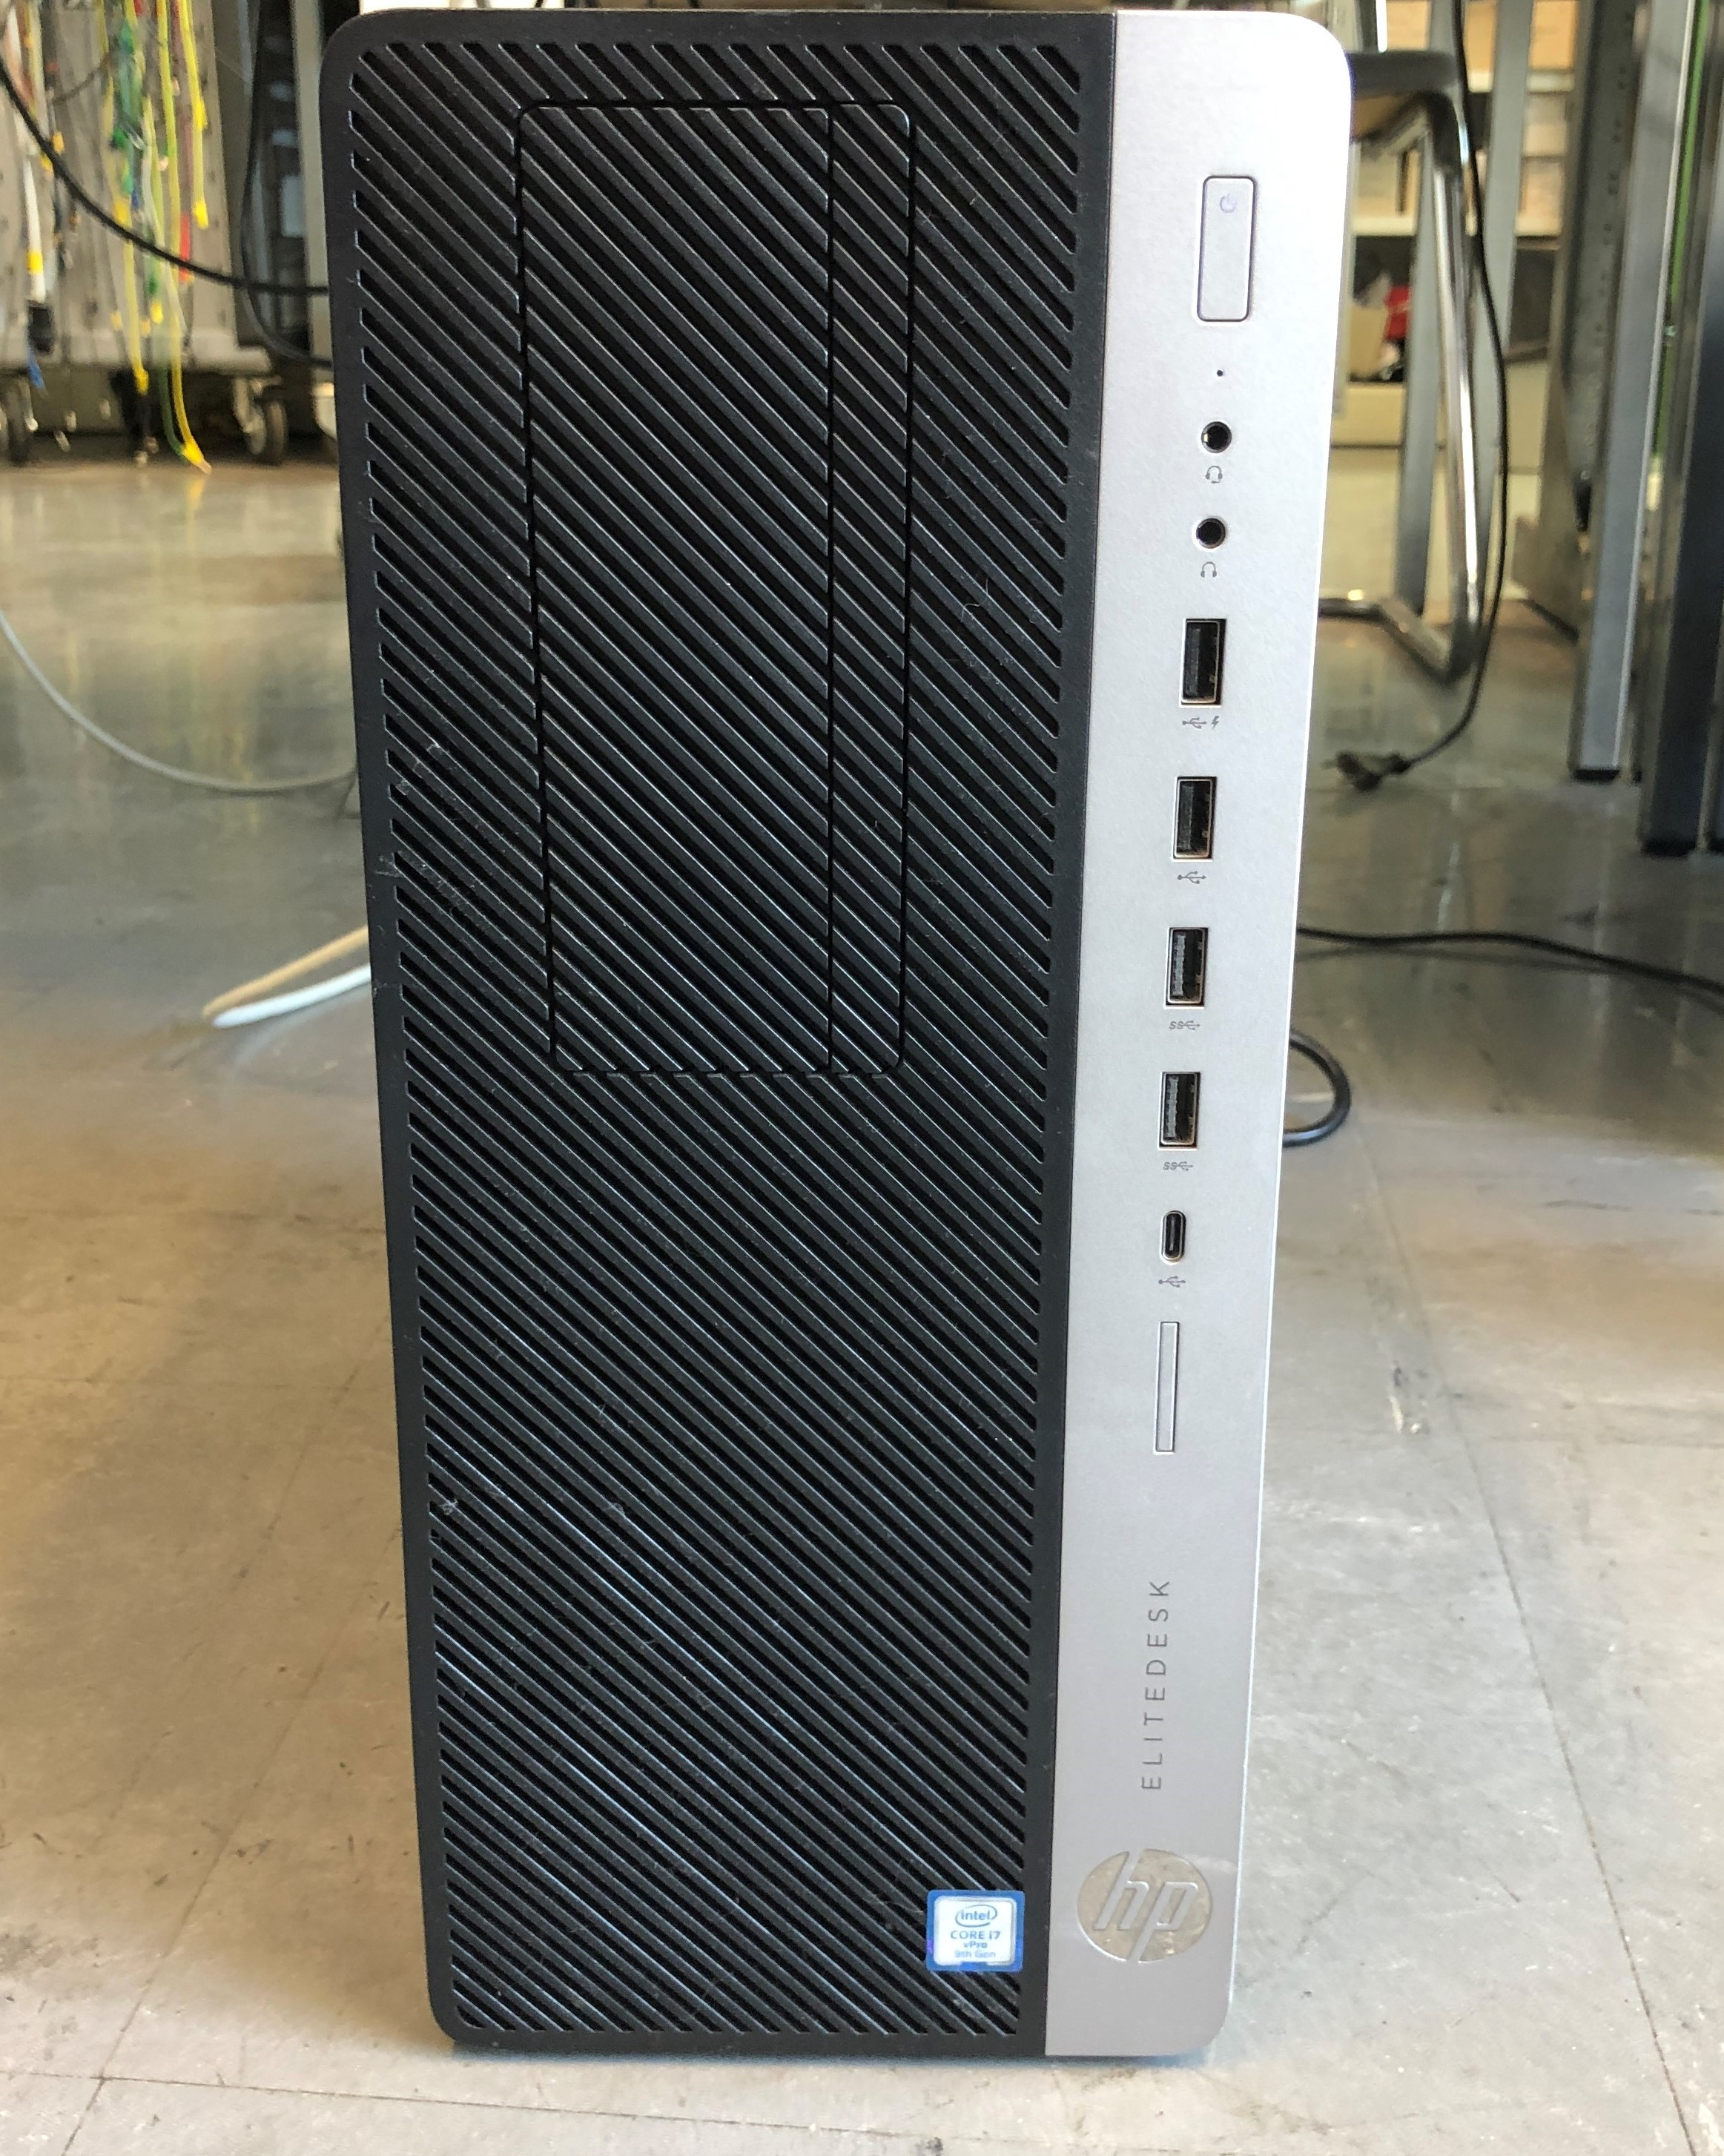
\includegraphics[width=1\textwidth]{Graphics/remPCfront.jpg}
     \end{subfigure}
     \hfill
        \caption{Pictures of the remote PC.}
        \label{fig:three graphs}
\end{figure}


\subsection{The EMP}

As mentioned earlier, the EMP is intended to interface with up to 12 EMCI's. This is done in a star topology. The EMCI acts as a processor for the EMCI's, which receive and send data to FE components in the detector.

\noindent The EMP is connected to the a PC by UART. This is necessary to pass the bootargs to the EMP upon booting and further to write the credentials. After booting, the EMP can be accessed through SSH if preferred. The firmware of the EMP is currently being prepared on the following modules:
\begin{itemize}
\vspace{-0.1 cm}
    \item Zynq UltraScale+ TE0807 (XCZU4EG-1E) \cite{MPSoCMod51:online}
    \vspace{-0.2 cm}
    \item Trenz Electronic TEBF0808 carrier board \cite{TrenzEle6:online}
\end{itemize}
\vspace{0.2 cm}
\noindent Where technical reference manual can be seen below:
\begin{itemize}
\vspace{-0.1 cm}
    \item Trenz Electronic TEBF0808 carrier board \href{https://wiki.trenz-electronic.de/display/PD/TEBF0808+TRM}{here}
\vspace{-0.2 cm}
    \item Zynq UltraScale+ XCZU4EG-1E \href{https://wiki.trenz-electronic.de/display/PD/TE0807+TRM}{here}
\end{itemize}
\vspace{0.2 cm}
\noindent The PS (processing system) of the EMP is a Linux-based OS. The version installed is CentOS Stream 8. The environment setup is made by Paris and can be seen in the GitLab repository \cite{EMCIEMPe95:online}. 

\noindent One crucial thing to take away here is that the file system of the EMP is not actually in the EMP memory but stored on the remote PC due to the NFS. 

\begin{figure}[H]
    \centering
    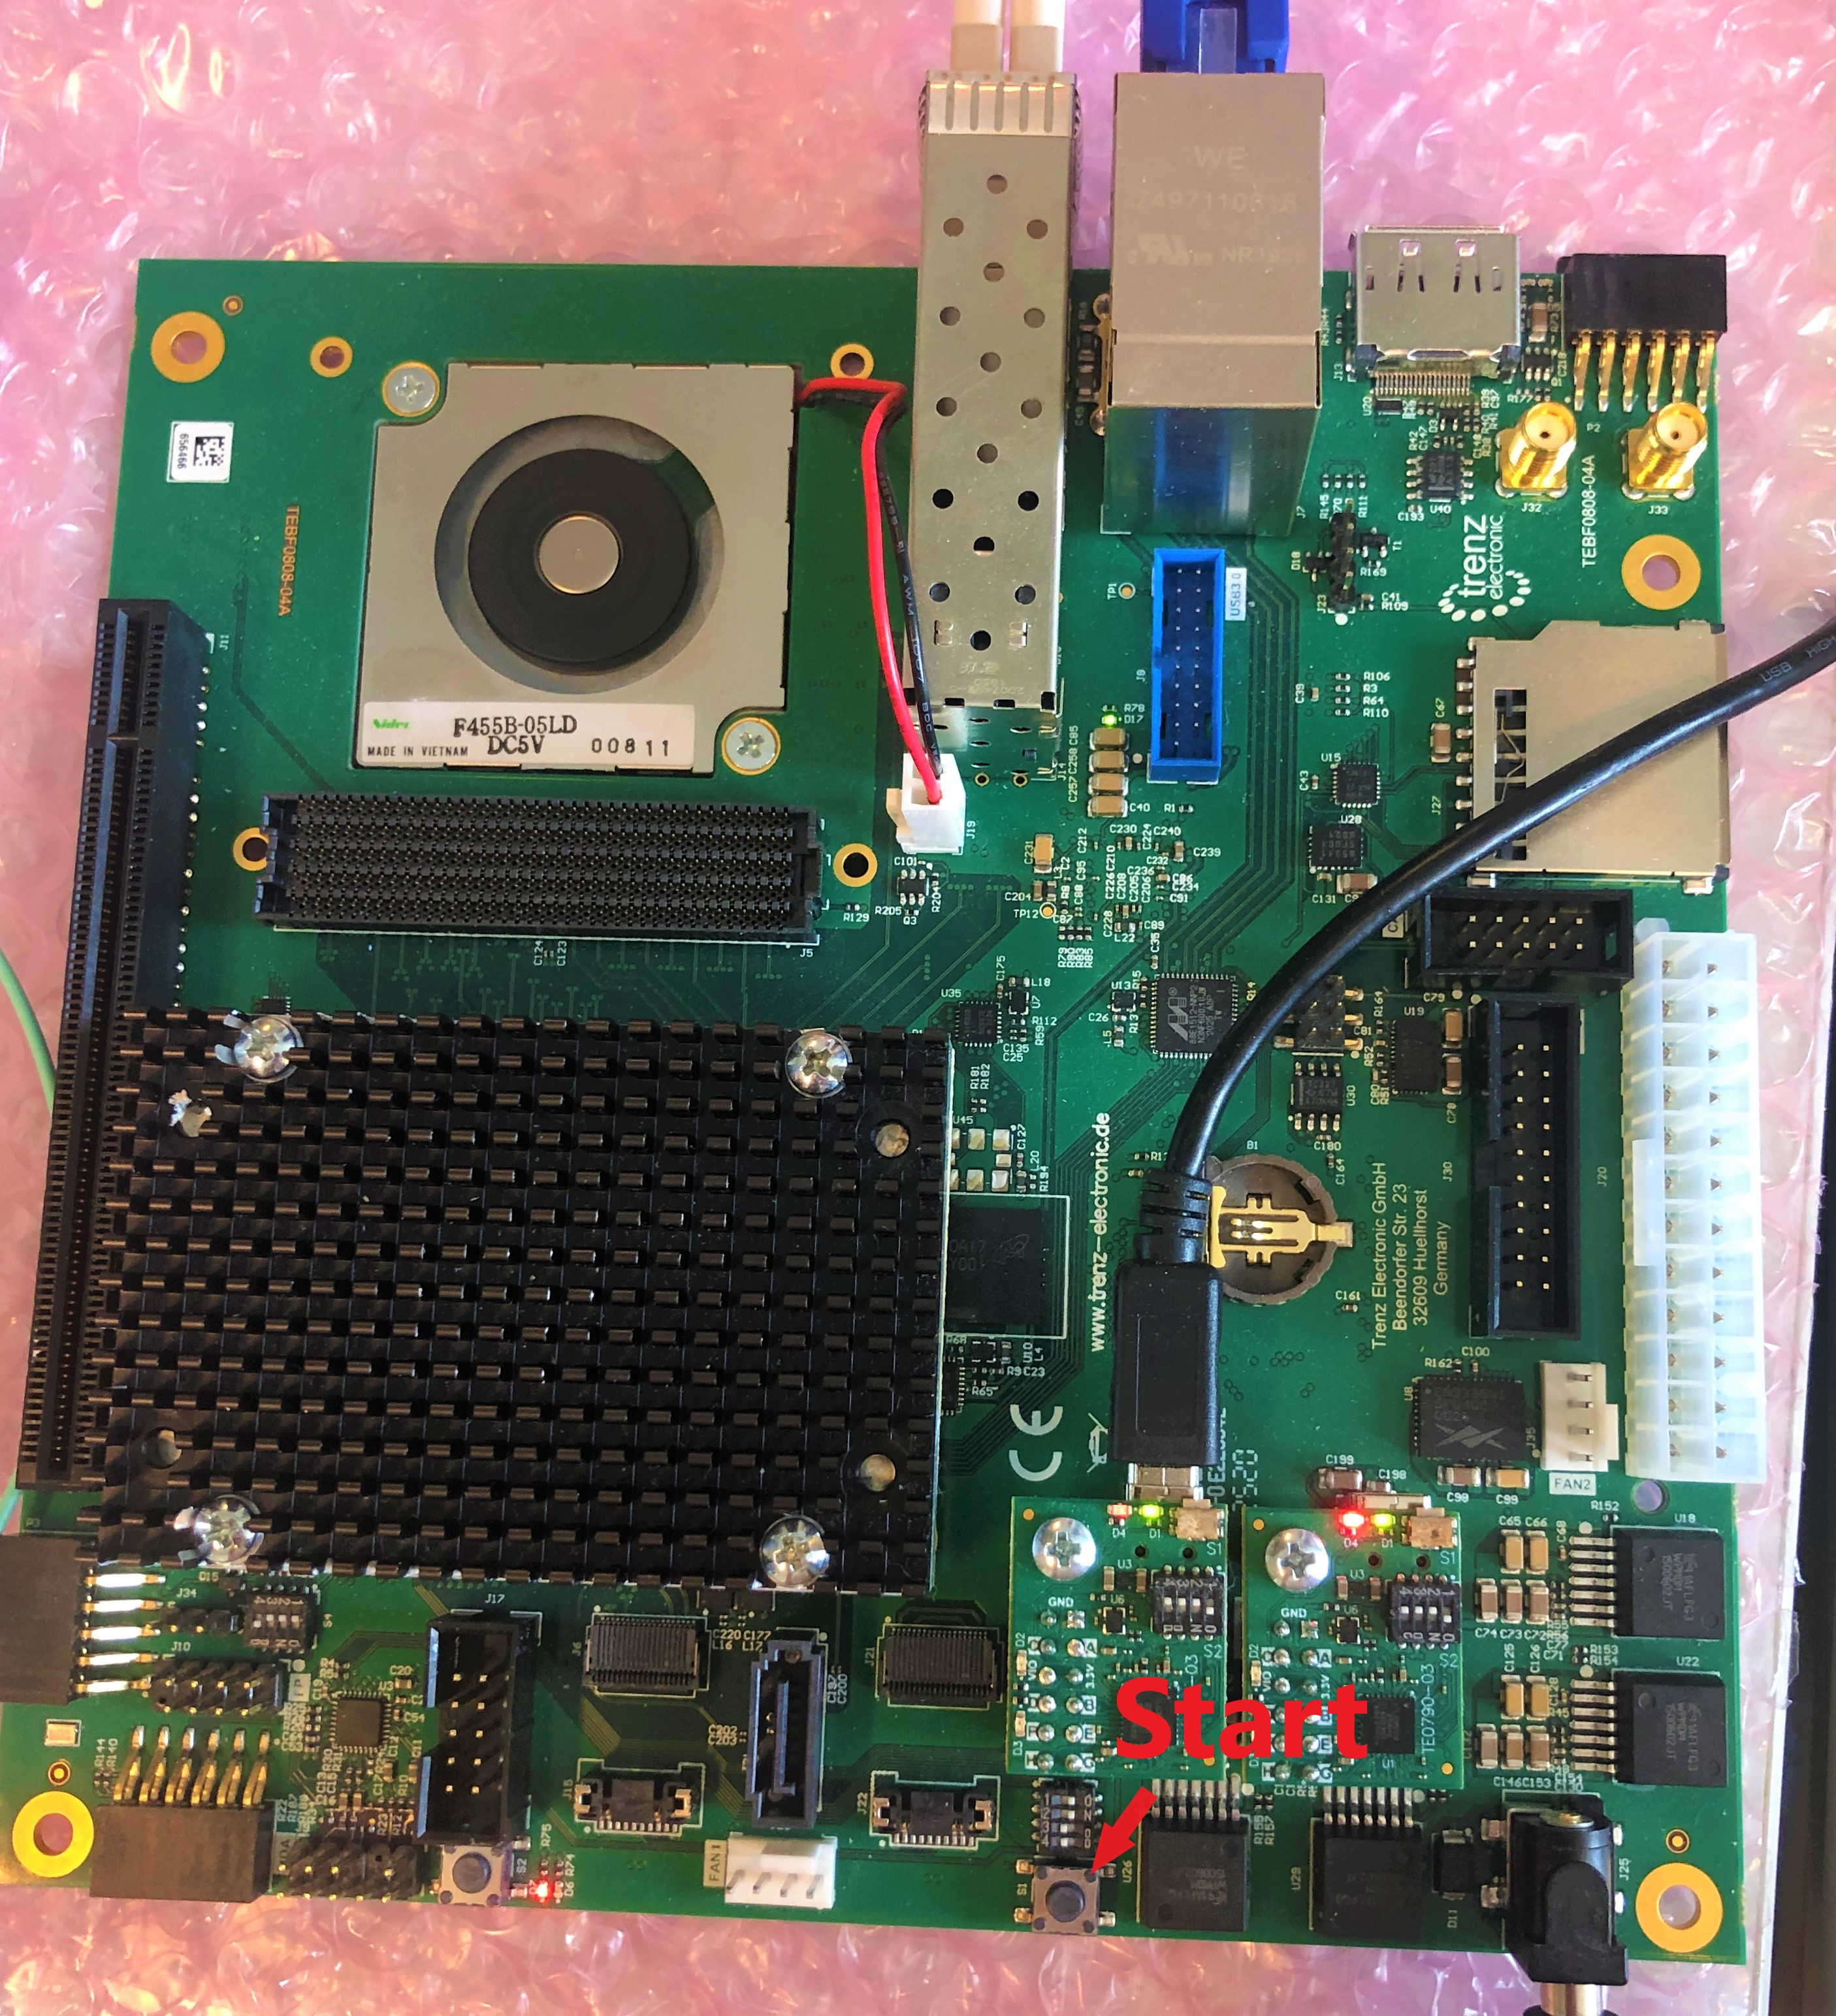
\includegraphics[width=1\textwidth]{Graphics/EMP_start.jpg}
    \caption{Top view of the EMP (Start marked).}
    \label{fig:EMP_start}
\end{figure}
\newpage
\subsection{The EMCI}

The EMCI works as an interface for controlling and monitoring the data sent and received between FE components and the EMP and is based on the lpGBT \cite{lpGBTMan75:online}. \\

\noindent For configuration of the lpGBT, the EMCI is currently connected through a wire to the PiGBT. This is also what is currently powering the EMCI. Alternatively, the power input can be provided through the FMC connector. 

\begin{figure}[H]
    \centering
    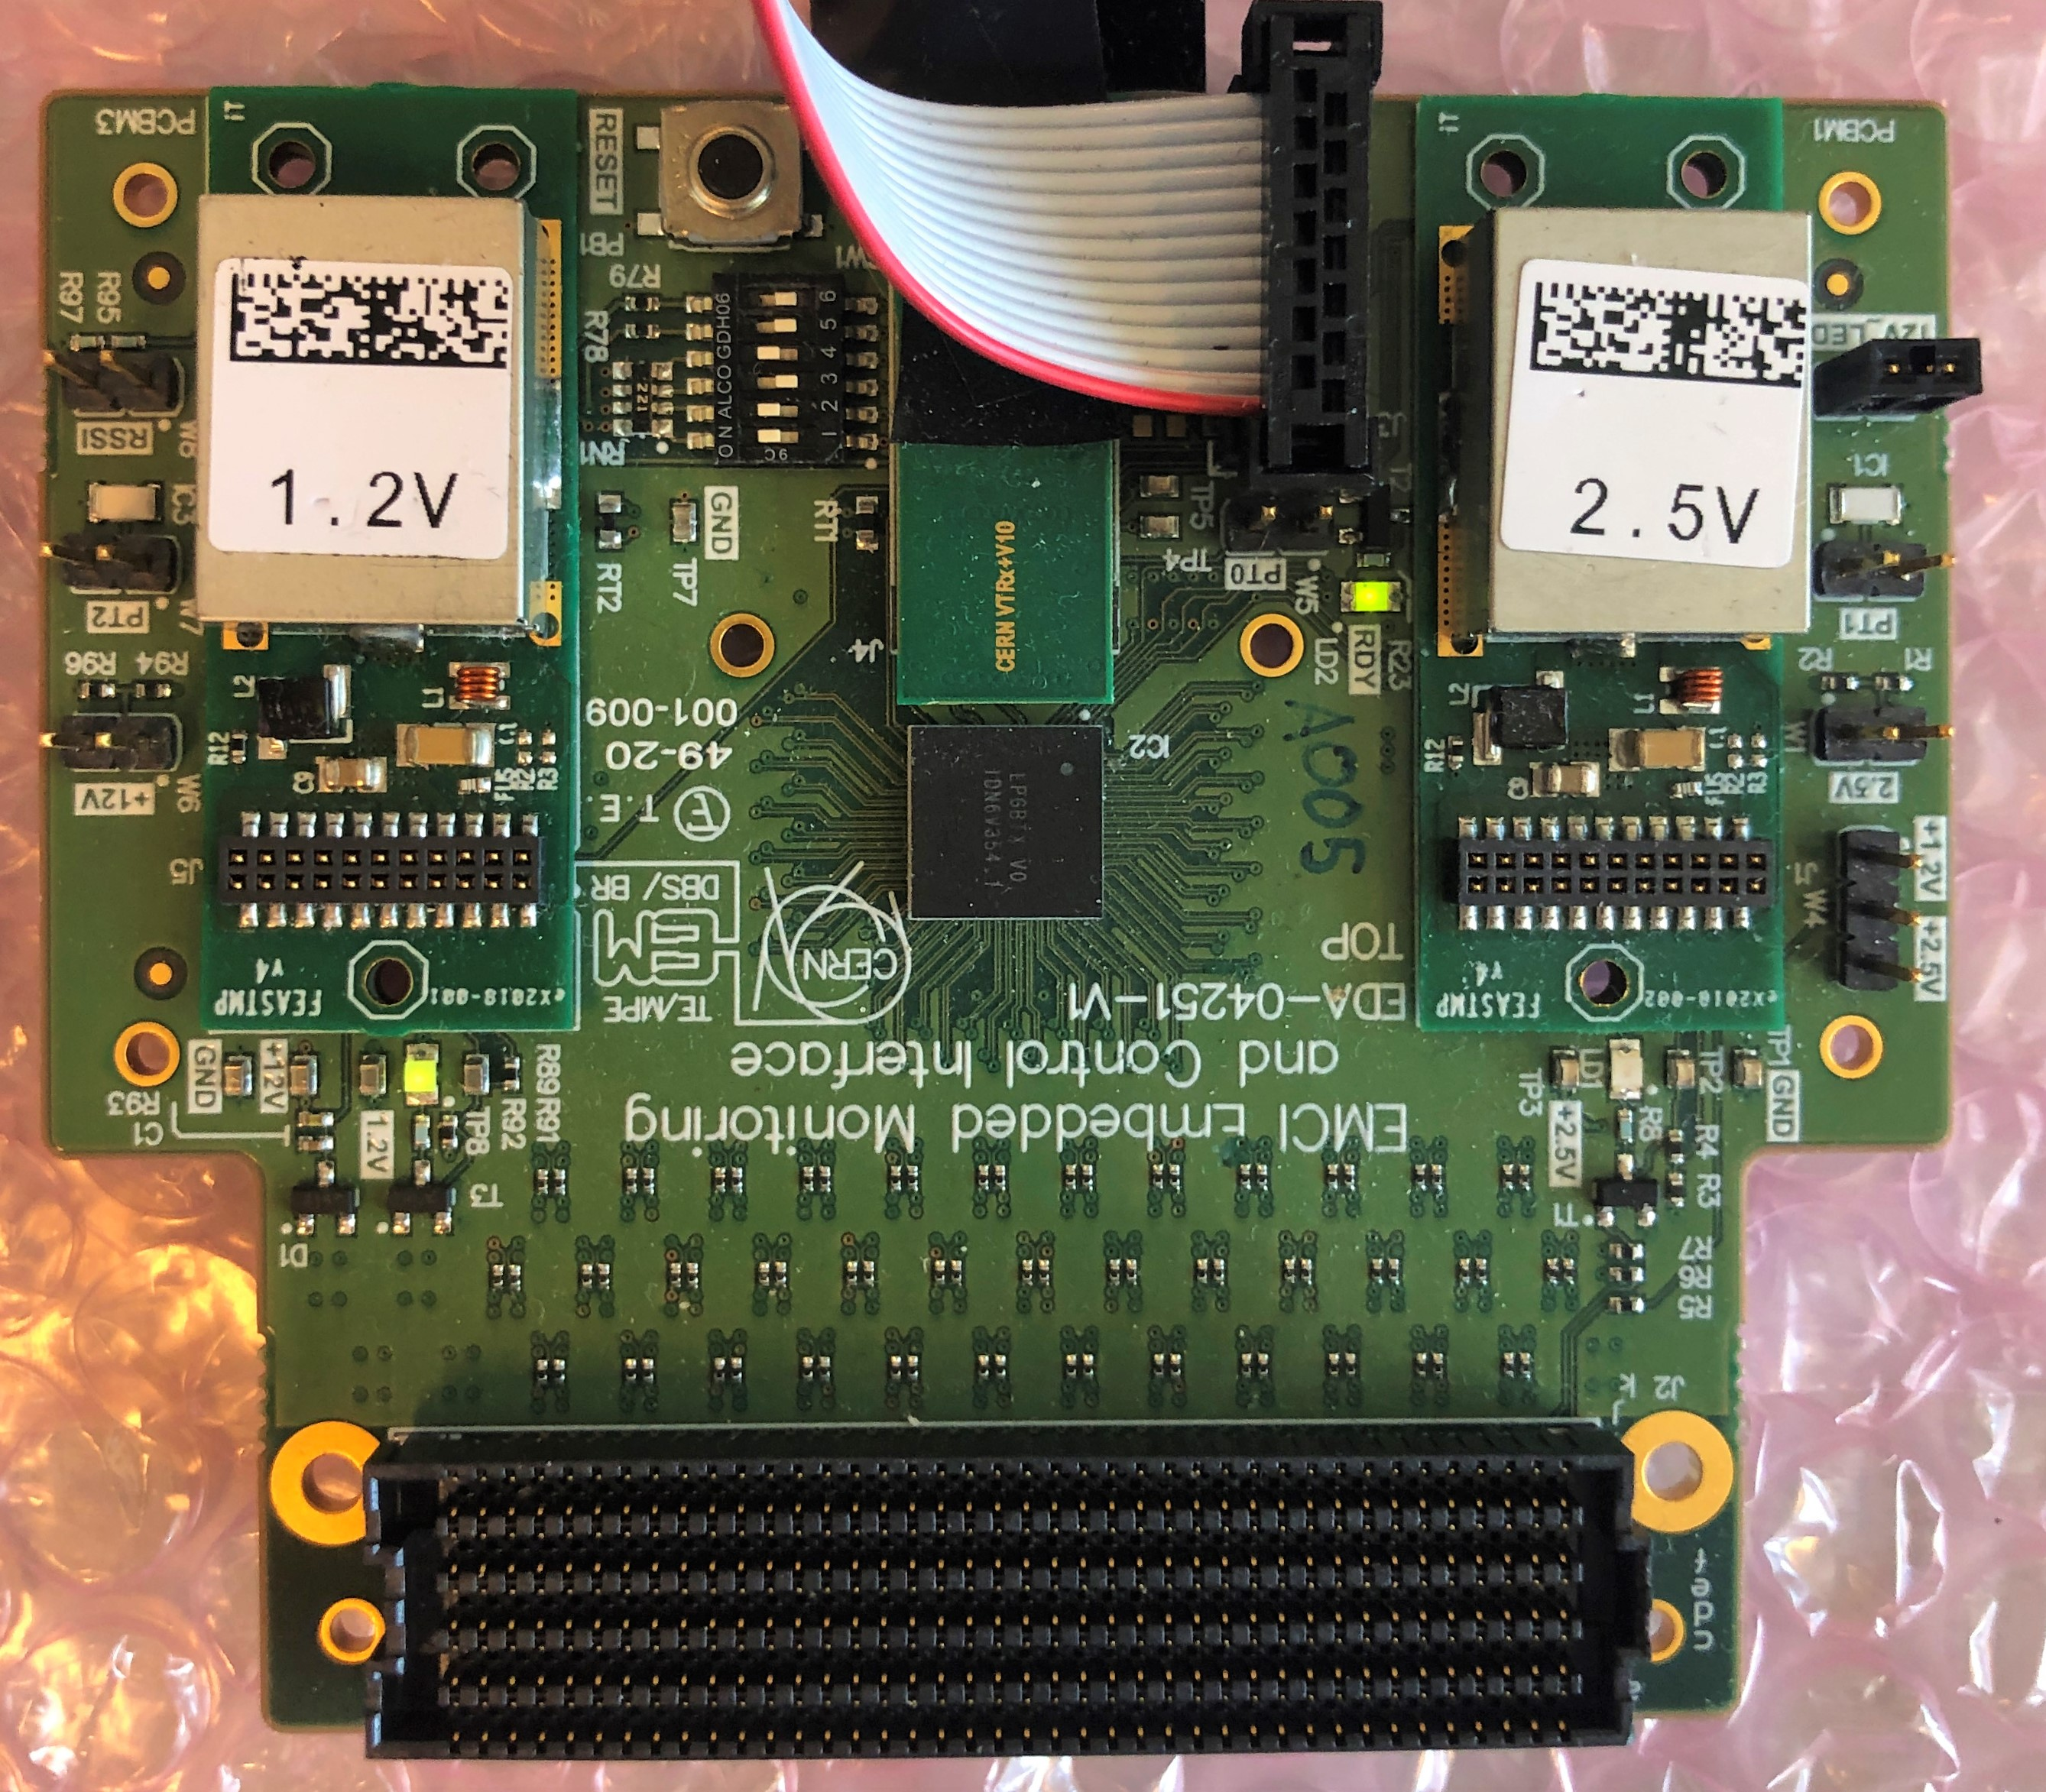
\includegraphics[width=.85\textwidth]{Graphics/EMCI.jpg}
    \caption{Top view of the EMCI.}
    \label{fig:EMP_start}
\end{figure}

\noindent The EMCI uses DIP switch one to six to preset the lpGBT operation mode. For my use, it is only necessary to know that DIP switch six controls the interface by which the lpGBT should be configured. \\

\noindent When it is in the \textbf{on} position, it allows configuration from the I2C slave. When it is in the \textbf{off} position, it allows configuration from the remote serial high-speed link.

\noindent As a result of this, the DIP switch six has to be turned \textbf{on} to configure the EMCI through the PiGBT. Likewise, it has to be \textbf{off} to communicate with the EMP. \newpage

\subsection{The PiGBT}
The PiGBT runs on a customized Raspberry Pi 4. It can be accessed out of the box through a web browser to ease the development process of the lpGBT \cite{VLDBcont6:online}. The web page can be accessed by entering the IP address displayed on the LCD of the component followed by the port. E.g. http://128.141.94.188:8080\\

\noindent The PiGBT is not meant to be used in the final production environment. 

\begin{figure}[H]
    \centering
    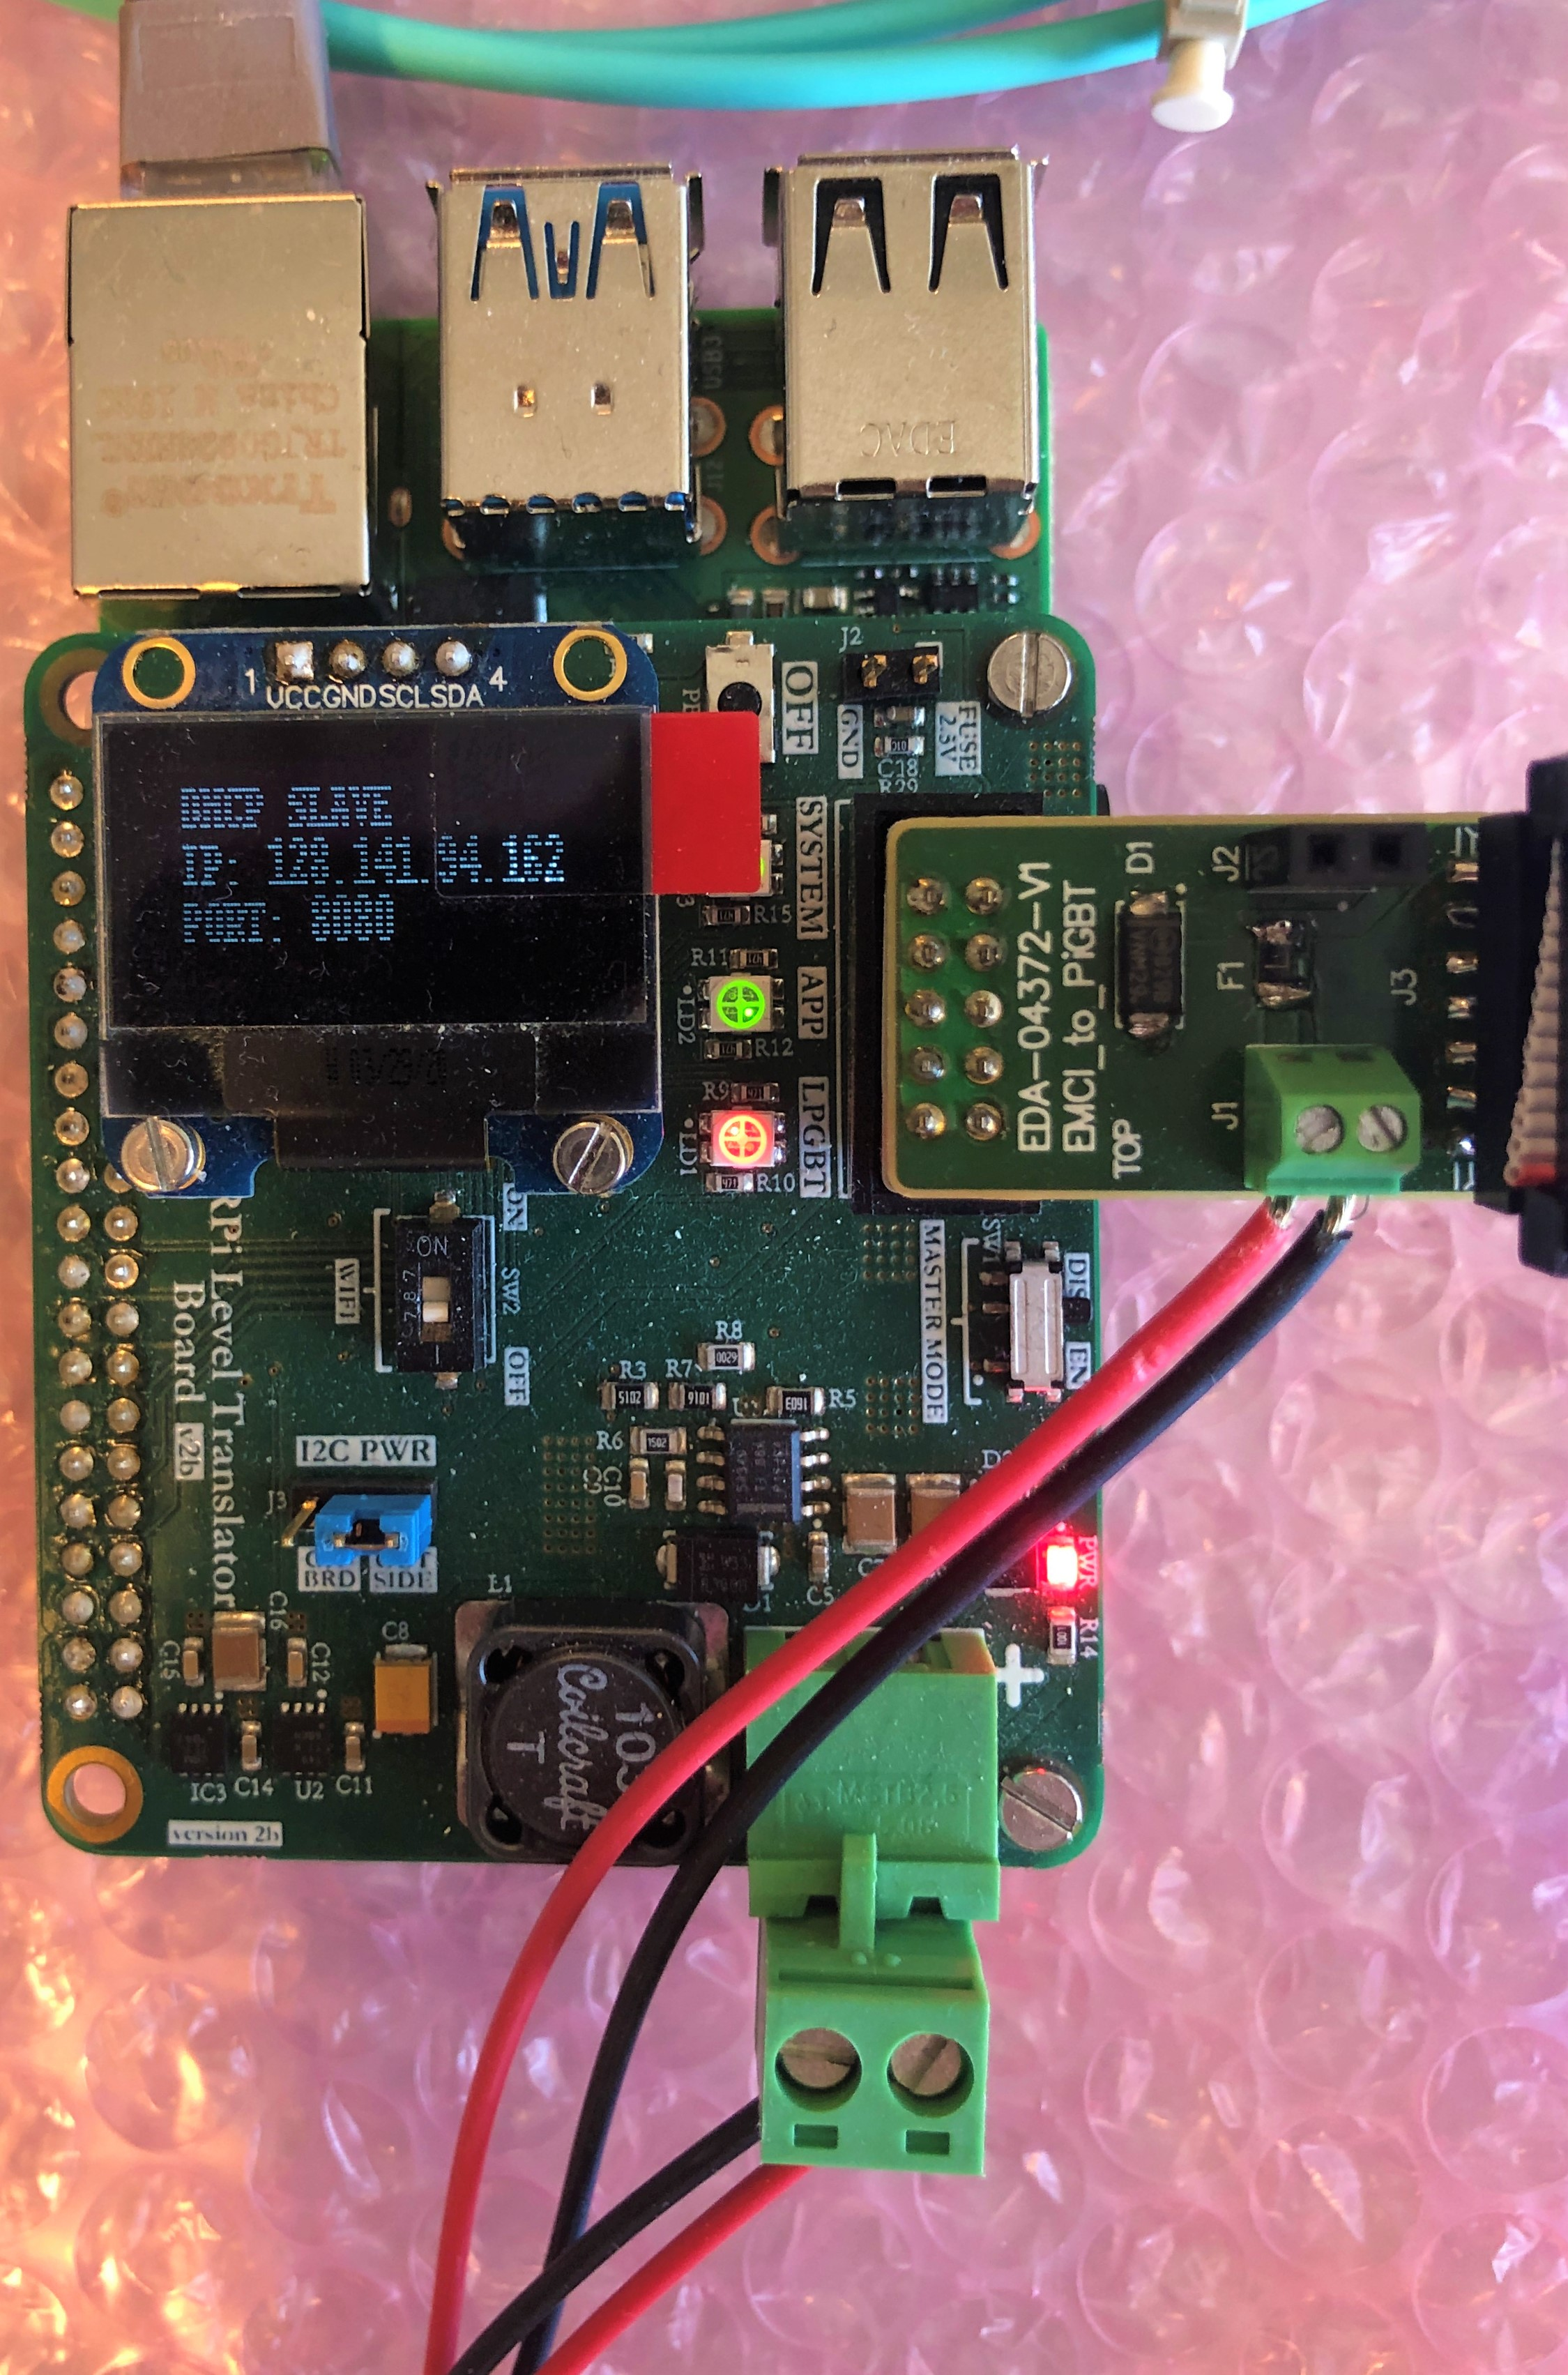
\includegraphics[width=.8\textwidth,angle=90]{Graphics/PiGBT.jpg}
    \caption{Top view of the PiGBT.}
    \label{fig:EMP_start}
\end{figure}
\newpage
\section{The complete EMP-EMCI setup}
A sketch showing all connections of the complete EMP-EMCI system can be seen below in figure \ref{fig:2243}.

\begin{figure}[H]
    \centering
    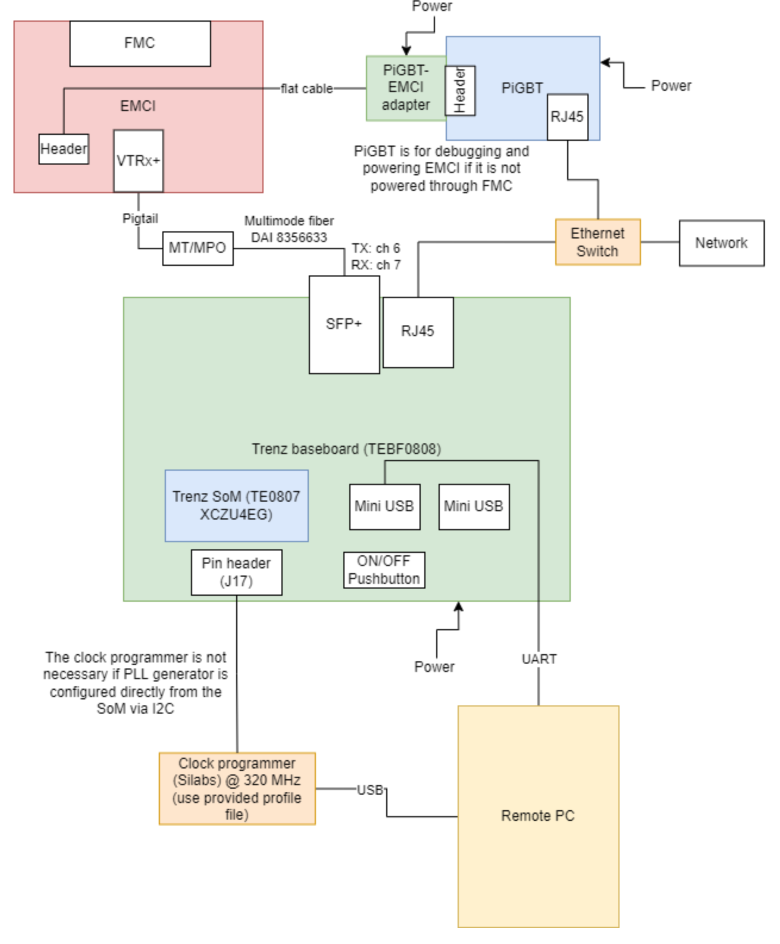
\includegraphics[width=.9\textwidth]{Graphics/pic_3.png}
    \caption{Sketch of the EMP-EMCI system.}
    \label{fig:2243}
\end{figure}

\noindent However, the Silabs Clock Programmer is not needed any longer. Below is a picture of the current setup. 

\begin{figure}[H]
    \centering
    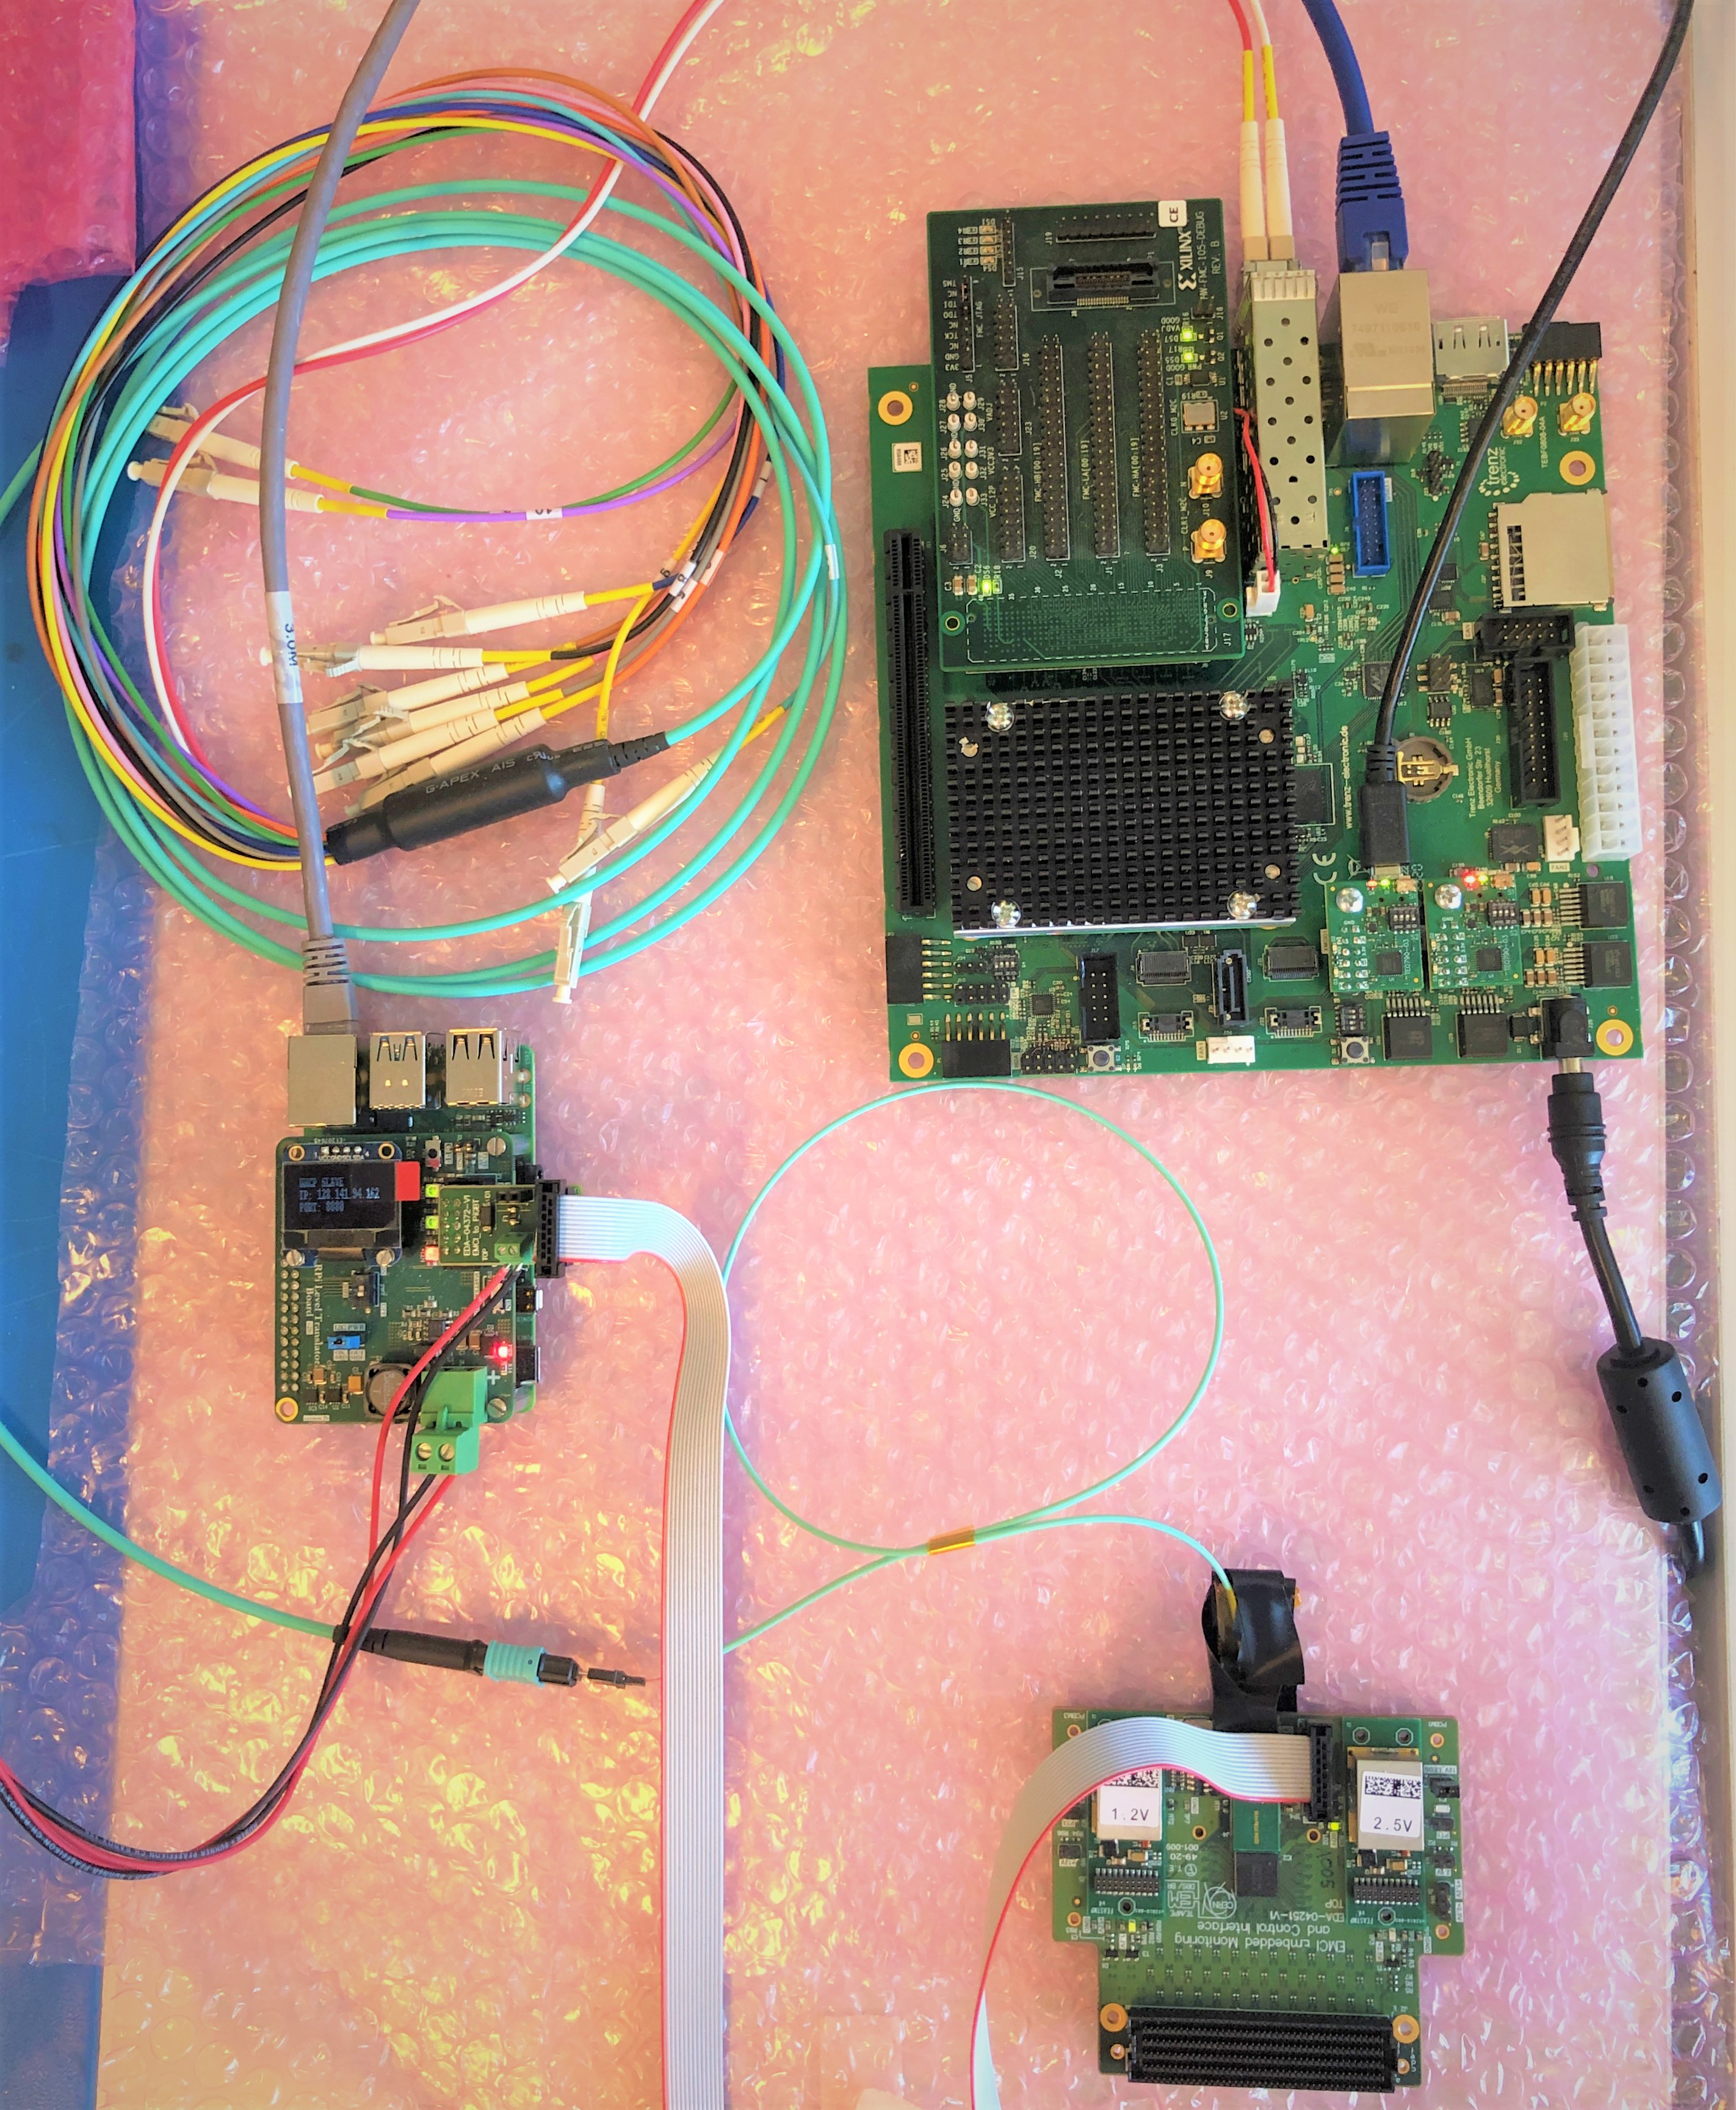
\includegraphics[width=.7\textwidth, angle=90]{Graphics/empemcipigbt.jpg}
    \caption{Top view picture of the EMP-EMCI system.}
    \label{fig:EMP_start}
\end{figure}

\chapter{Work areas}

My first work assignment was to be familiar with the hardware. Here there was much stuff to dive into, as this involves the hardware specifications of the EMP, EMCI, LpGBT, and PiGBT. Furthermore, I had to understand the systems and tools used. \\

\noindent From here, I could begin to develop some small programs. This also supports the understanding of the cross-compilation and the VIM tool. I had no experience in several of these subjects before I started, which at first made it challenging to begin developing. Nevertheless, the approach here was to pick up the pieces along the way with a "learn by doing" mentality. \\

\noindent The work done during my internship and represented in this report are:

\begin{itemize}
    \item Development of the temperature monitoring of Zynq
    \item Development of the clock configuration
    \item Development of the GPIO test
\end{itemize}

\noindent Apart from these three tasks, much work has been done in the error handling of unexpected failures. Several failures occurred during my time at CERN, which I had to prioritize. These failures are:

\begin{itemize}
    \item Failure of the Remote PC
    \item Failure of booting the EMP from NFS
    \item Failure of the Remote PC - the second time
\end{itemize}

\noindent I will not get deep into handling these failures, as the focus of this report will be the development. Nevertheless, it will briefly be mentioned here.

\subsection*{Error handling}
\noindent Searching for issues and solving them can be tedious as no actual progress is made. However, it helps obtain a deeper understanding of the system's mechanisms and hardware. In my case, I spent a lot of time examining the Linux OS to get the knowledge required to determine if an error could - or could not - be caused by what I thought could be an issue. Most of the time, the error handling process was done by trial and error, born from the belief of what may cause the error. Unfortunately, the bigger the system, the more complex the searching is. For that reason, I started with the easy-to-solve possibilities first. It further shrinks down the essence of the cause by confirming what is working and what doesn't. If fortunate, one might obtain an indication in the shrinking process of what is the reason. When the cause is known, it is often manageable to find out what to do, either by using the internet to obtain knowledge or by reaching out to colleagues.

\section{Development of the temperature monitoring of Zynq} \label{sc:temp}
Daniel made a suggestion to develop a program to monitor the registers written to the EMCI from the EMP and to display this data in a GUI. But as the EMP is limited in its processing power, it is preferred not to use the EMP to run the GUI. This means another machine has to host the GUI while the EMP provides the data. By that means, the program will need a way of transferring the data. \\

\noindent As the GUI and the communication mechanisms are crucial in this application. It was chosen first to make a minor program to illustrate these mechanisms as a proof-of-concept. This proof-of-concept program was the program for monitoring the temperature of the Zynq processor. Besides being a proof-of-concept for a later project, an easy way to monitor the temperature of the Zynq can be advantageous.

\subsection*{Objective of the program}

The program should have two executable files: One for the host and one for the client. The code for the host will be made in Python to utilize the effective GUI library - Qt. On the other hand, the client should be made in C++, as the language is faster and the resources are little on the EMP.\\

\noindent The program should allow communication between the EMP and a host PC. Communication should be established to allow data from the EMP concerning the temperature to be sent to the host. Furthermore, the data sent from the C++ should be converted so that Python can use it. \\

\noindent The GUI should appear as a small window with the temperatures of the Zynq chip. The Zynq has three temperature sensors, one for the programmable logic (PL) and two for the processing system (PS). The GUI should show all three and update their values every second. Furthermore, it could be "nice-to-have" information showing the allowed temperature interval. \\

\subsection{Creating the code}

As mentioned, the code should show the temperature for the Zynq processor, more specifically, the Xilinx ZYNQ UltraScale+ ZU7EV-1FBVB900E. This temperature data is found in the SYSMONE4 architecture present on the Zynq, which provides the three temperature sensing channels;  One in the low power domain (LPD), one in the full power domain (FPD), and one in the programmable logic (PL). \\

\noindent 
The program will use a TCP socket to send the data fetched from the EMP's Zynq's SYSMONE4 architecture and convert this data to a readable temperature - in Celcius - using equation 2-12 on page 41 in \href{https://china.xilinx.com/content/dam/xilinx/support/documents/user\_guides/ug580-ultrascale-sysmon.pdf}{this report}. The equation is also shown here:
((data\_fetched * 509.3140064)/65536.0)-280.23
When the data is converted, it is sent to the server, where the host will display the measured temperature.\\

\noindent As mentioned above, the code is split into two separate files. These two files are named temperatureMonitor\_server.py and temperatureMonitor\_client.cpp. A brief explanation of the purpose of the two files is given below. 

\paragraph{temperatureMonitor\_client.cpp} \hspace{-0.3 cm} This file is supposed to run on the EMP, and is responsible for sending the data to the server. It is also the code responsible for fetching the data from the SYSMONE4. 

\paragraph{temperatureMonitor\_server.py} \hspace{-0.3 cm}
This file is meant to run on the host, the computer to operate the GUI. It is responsible for the GUI, and with multi-threading, it updates the GUI every time new data is received. \\

\noindent The source code of the two files can be seen in appendix \ref{app:D} and appendix \ref{app:E}.
 
\subsection*{Usage}

\begin{enumerate}
    \item Make sure that the IP address of your server matches the IP address given in the code
    \vspace{-0.2 cm} 
    \item Run temperatureMonitor\_server on the remote PC.
    \vspace{-0.2 cm} 
    \item Run temperatureMonitor\_client on the EMP.
\end{enumerate}

\noindent If everything goes well, the user will get a confirmation in the terminal, and a small window with the temperature will appear, as shown in figure \ref{fig:guis} and figure \ref{fig:printss}.\\

\begin{figure}[H]
    \centering
    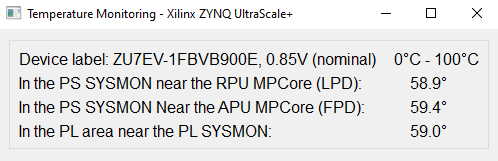
\includegraphics[width=.8\textwidth]{Graphics/GUI.PNG}
    \caption{Screenshot showing the GUI for the program.}
    \label{fig:guis}
\end{figure}

\begin{figure}[H]
     \centering
     \begin{subfigure}[b]{0.49\textwidth}
         \centering
         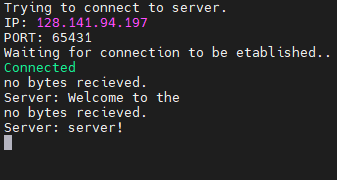
\includegraphics[width=1\textwidth]{Graphics/print_in.PNG}
     \end{subfigure}
     \hfill
     \begin{subfigure}[b]{0.49\textwidth}
         \centering
         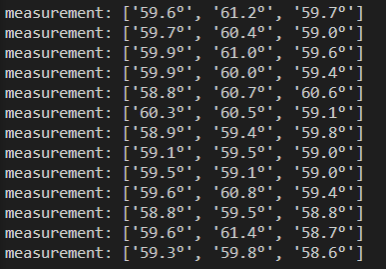
\includegraphics[width=1\textwidth]{Graphics/print_out.PNG}
     \end{subfigure}
     \hfill
        \caption{Console print out - From respectively Server (left) and client (right). }
        \label{fig:printss}
\end{figure}

\newpage

\section{Development of the clock configuration} \label{dev:codeclk}

As the EMP boots, it is necessary to configure the clock present on the board before the EMP can communicate with the EMCI. The current solution to configuring the clock is to use the ClockBuilder toolkit from Silabs. The kit consists of a field programmer mainboard connected between the PC and the Trenz baseboard, which allows the user to configure the clock via software supported by Silabs - named Clockbuilder PRO.\\

\noindent The problem with this solution is that the clock needs to be reconfigured every time it boots, and reconfiguring the clock with Silabs Clockbuilder PRO can be tedious. It is also desired to make the EMP independent on the Silabs Clockbuilder kit and avoid adding more wiring to the EMP than necessary. The setup when using the Silabs Clockbuilder PRO is shown in figure \ref{fig:Silabstoolkit} below. 

\begin{figure}[H]
    \centering
    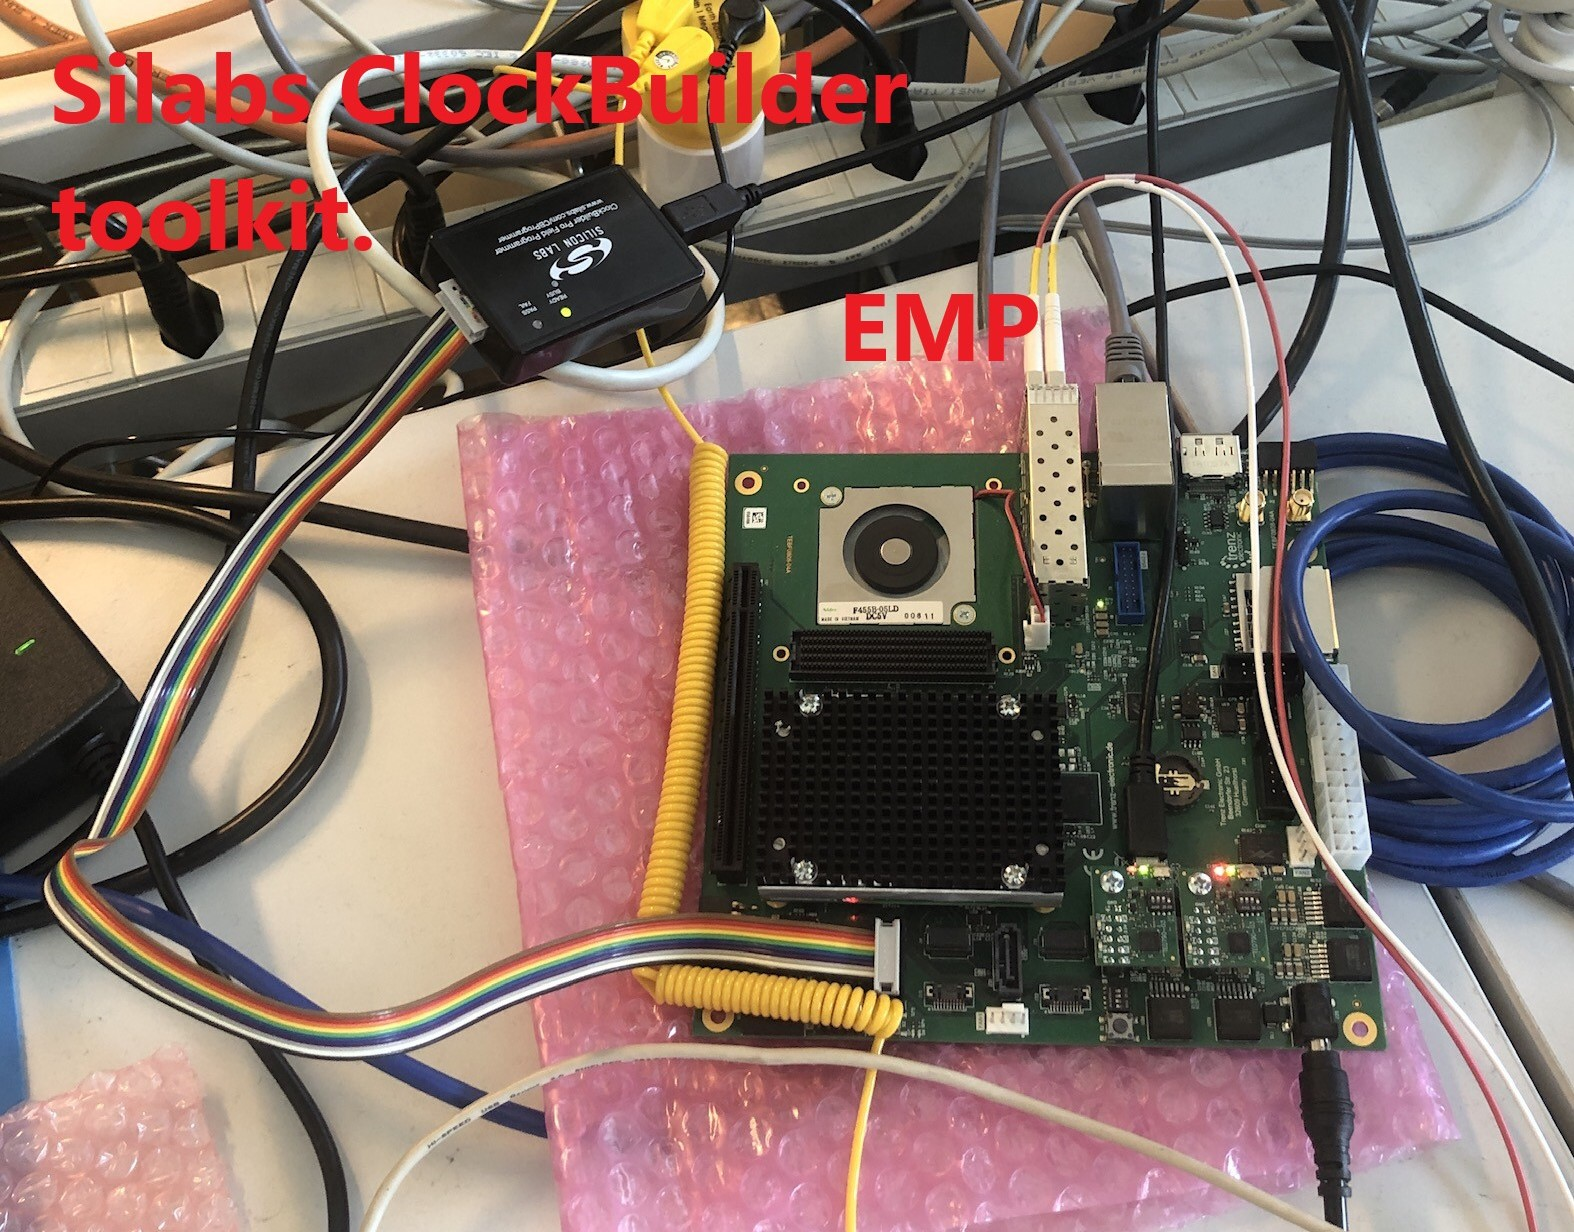
\includegraphics[width=.75\textwidth]{Graphics/IMG_0312.jpg}
    \caption{Setup of EMP connected to the Silabs toolkit.}
    \label{fig:Silabstoolkit}
\end{figure}


\noindent A more convenient way is to make a program that allows the EMP to configure the clock itself. To do this, the Xilinx Zynq Ultascale chip, placed on the Trenz baseboard, has to communicate with the On-module Quad programmable PLL clock generator Si5345 (TE0808), which is done with the use of I2C. In between the Xilinx chip and the clock generator is an 8-channel I2C switch (U27). From the manual, it is found that the address to write to is 0x69 \cite{TEBF080828:online}. An overview from the manual is shown in figure \ref{fig:overview}.

\begin{figure}[H]
    \centering
    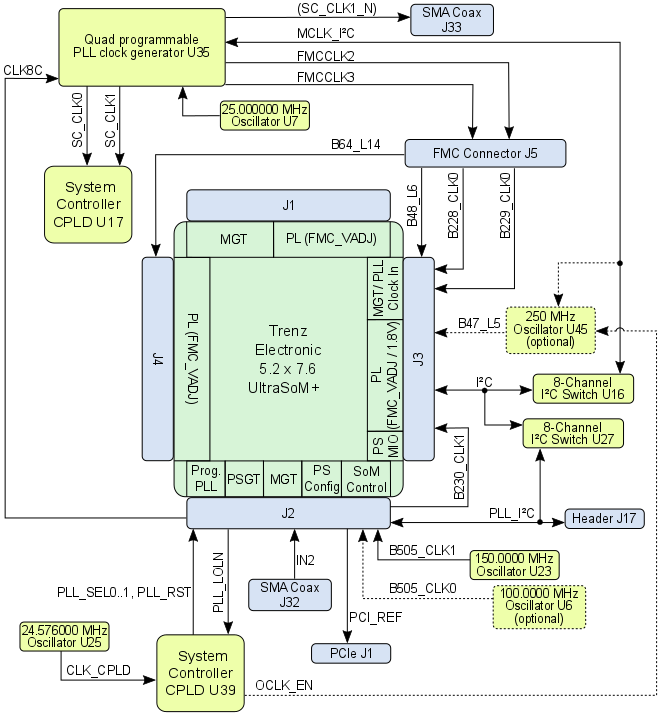
\includegraphics[width=.85\textwidth]{Graphics/BD-TEBF0808_Clocking.png}
    \caption{Overview of the clocking configuration on carrier board .}
    \label{fig:overview}
\end{figure}

\noindent Now that the slave address is known, it is possible to write some code to communicate with the clock generator. The first thing to do in the code is to collect a list of registers and values to write to. Fortunately, it is possible to export the configuration file from ClockBuilder to C. This makes the configuration a lot easier. The file exported is seen in appendix \ref{app:B}.\\

\noindent Now that we have the data, we need to manipulate it to fit this application. 

One problem occurring here is that the register address we have to write to is 16-bit (e.g., the value 0xFFFF); it is an issue because the I2C only handles 8-bit. So to solve this problem, the special 'page register' with the address 0x0001 is used. The 'Page Register' allows the user to select between 256 possible pages. To select a page - e.g., page 1 - first write 0x01 to the page register 0x01, and directly the page will be selected. The attribute of the 'page register' is that page 1 will start from the address where the previous page (page 0) ended. This means that page 0 begins from the address with the decimal value of 0 and goes up to 255. Page 1 begins from address 256 and goes up to 511,  page 2 begins from 512 and goes up to 767, and so on. So if we want to write to, e.g., register 0x0B24. We first have to select the page 0xB by writing 0xB to 0x01 (the Page Register) and then write to the address 0x24. In this manner, it is possible to write to 16-bit addresses without exceeding the data limit for the I2C of 8 bit.\\

\noindent For the above reason, the 16-bit register address, given from the exported ClockBuilder file, has to be split into two 8-bit addresses. The upper 8-bit will be the value of the page, and the lower 8-bit will be the value of the register address.\\

\noindent As The C function named 'extractData()' handles the data from the ClockBuilder file and is shown in listing \ref{listing:3}. Here the function returns an $n \times 3$ matrix, where the first column in the matrix is the value of the page. The second one is the value of the register, and the third one is the value to write.\\  

\begin{figure}[H]
\centering
$\begin{vmatrix}
Page\:Address & Register\:Address & Value\\
\vdots & \vdots & \vdots\\
Page\:Address & Register\:address & Value
\end{vmatrix}$
\caption{$n \times 3$ Matrix returned by function \mintinline{html}{extractData()}.}
\end{figure}


\begin{listing}[H]
\begin{minted}[
        frame=single,
        obeytabs=true,
        tabsize=1,
        linenos,
        numbersep=10pt,
        highlightlines={},
        highlightcolor=newyellow]
        {c}
int **extractData() {

	uint8_t bytes[2];
	uint16_t addr;

	/* Numbers of elements in array */
	size_t array_size = sizeof(si5345_revb_registers)/8;

	/* allocating rows */
	int **arr=(int **)malloc(sizeof(int *)*array_size);

	/* initialize matrix: data_set[row][column] */
	int data_set[array_size][3];
	int column = 0 ;

	/* Writes data to matrix from Silabs design report */
	for (int row = 0 ; row < array_size ; ++row) {

			/* allocating columns */
			arr[row] = (int *)malloc(sizeof(int)*array_size);

			/* splits 16 bit into two 8-bits */
			addr = si5345_revb_registers[row].address;
			bytes[0] = addr >> 8; // high byte
			bytes[1] = addr & 0x00FF; // high byte

			/* writes address data first 8-bit to page column */
			arr[row][column] = bytes[0];
			
			/* writes address data last 8-bit to reg. addr. column */
			column=1;
			arr[row][column] = bytes[1];

			/* writes address data to thrid column for value 0xD8 */ 
			column=2;
			arr[row][column] = si5345_revb_registers[row].value;
			column=0;
	}
	return arr;
}
\end{minted}
\caption{The function extracting the data from the ClockBuilder file.} \label{listing:3}
\end{listing}


\noindent After 'extractData()' has manipulated the data, the I2C has to be set up. Here take inspiration from a code made by Cosmin Tanisla\cite{linuxuse66:online} to get started. The code has some great functions there will handle the I2C and, in that regard, make the work more manageable.\\

\noindent A struct is created to set up the I2C. The struct consists of a device filename and a device address. The filename is the path of the I2C bus file in the EMP, which is found in the folder \mintinline{html}{/sys/class/i2c-dev/} on the EMP. In this application, we use the I2C-13. Additionally, the device address can be found in the Trenz baseboard manual as 0x69. The I2C device can now be started with the help of the functions provided by Cosmin Tanisla \mintinline{html}{i2c_start}. This is shown in line 17 in the code snippet below \ref{listing:a}.
\vspace{0.3 cm}
\begin{listing}[H]
\begin{minted}[
        frame=single,
        obeytabs=true,
        tabsize=1,
        linenos,
        numbersep=10pt,
        highlightlines={17},
        highlightcolor=newyellow]
        {c}
	int **data_from_emp_silabs;

	/* Fetching data from Silabs design report to an matrix */
	data_from_emp_silabs = extractData();

	/* Displays data in matrix */
	 show_data(data_from_emp_silabs);

	struct I2cDevice dev;

	/* Set the I2C bus filename and slave address,
	dev.filename = (char *)"/dev/i2c-13";

	/* clock generator Si5345 [U35] has slave address 0x69 */
	dev.addr = 0x69;

	i2c_start(&dev);
\end{minted}
\vspace{-0.6 cm}
\caption{The function extracting the data from the ClockBuilder file.} \label{listing:a}
\end{listing}
\noindent Now, it is possible to read or write data to the clock generator from the ClockBuilder file. The way this is implemented is with a \mintinline{html}{for loop}. The \mintinline{html}{for loop} starts from the first row of the matrix, fetching data from each column (page address, register address, value) and placing it into a corresponding 8-bit integer. This should not be necessary, but it makes the code more readable, in my opinion.\\

\noindent After the code is fetched into the corresponding variables, the value of the page is used in a switch case; its function is to control which page to write to. After that, the register is written with the corresponding value.\\

\noindent The following code sequence will read the data from the same register just written to validate that the writing was successful. If the value read from the register corresponds to the value just written, it is verified that the register successfully has been written. However, be aware that this is not always the circumstance. Some registers are self-clearing, implying that they will clear their value right after writing; hence the data is not saving the value just written - This must be considered when validating the data in the printout.

When the register is written, the \mintinline{html}{for loop} repeats the sequence, but for the next row, until the matrix ends. This can be seen in the code snippet \ref{listing:ad}. 

For clarifying, the code snippet shown here \ref{listing:ad} is not the complete code used, but is a shortened version to give the reader the basic idea of the essential concept. The whole code can be seen in the appendix \ref{app:F} and \ref{app:G}.
\vspace{0.3 cm}
\begin{listing}[H]
\begin{minted}[
        frame=single,
        obeytabs=true,
        tabsize=5,
        linenos,
        numbersep=10pt,
        highlightlines={},
        highlightcolor=newyellow]
        {c}
/* Calculate size of array from EMP_Silabs */
size_t array_size = size_of_array() - 1;
for (int i = 0; i < array_size; ++i)
{
	/* Fetch data from matrix */
	uint8_t page = data_from_emp_silabs[i][0];
	uint8_t reg = data_from_emp_silabs[i][1];
	uint8_t value = data_from_emp_silabs[i][2];
	switch (page)
	{
	case 0:
		i2c_write_reg(&dev, 0x01, 0x00);
		break;
    /* from 0 up to 11 */
	case 11:
		i2c_write_reg(&dev, 0x01, 0x0B);
		break;
	default:
		return -1;
	}
	i2c_write_reg(&dev, reg, value);
}
i2c_stop(&dev);
return 0;

\end{minted}
\vspace{-0.6 cm}
\caption{Describes the essential functionality of the code used for fetching data and writing it into registers.} \label{listing:ad}
\end{listing}
\noindent When the code is executed, it displays every register written. With the related information of page, register address, current value and written value, and most importantly, if the process succeeded. Further, the output gives insight into the phases of the writing. As mentioned earlier, the configuration has to follow a certain sequence. This sequence is split into three phases: The preamble, the registers to be written, and the postable. A code snippet is shown in listing \ref{listing:4}.
\vspace{0.4 cm}
\begin{listing}[H]
\begin{minted}[
        obeytabs=true,
        frame=single,
        %framesep=2mm,
        tabsize=1,
        %numbersep=12pt,
        %fontsize=\footnotesize,
        %baselinestretch=1.2,
        %bgcolor=backcolour,
        %linenos
        %highlightlines={},
        %highlightcolor=newyellow
        ]
        {bash}
Start configuration preamble
*********************************************************************
  Action:       Page:   Register:   Value:    Writing:     Status:
*********************************************************************
  [Wrote]        B       0x24        0xDB      0xD8       [Success]
  [Wrote]        B       0x25        0x2       0x0        [Success]
  [Wrote]        5       0x40        0x0       0x1        [Success]
*********************************************************************

 Start configuration registers
*********************************************************************
  Action:       Page:     Register:   Value:    Writing:     Status:
*********************************************************************
[Overwrote]      0       0xB         0x68      0x68       [Success]
[Overwrote]      0       0x16        0x2       0x2        [Success]
[Overwrote]      0       0x17        0x1C      0x1C       [Success]
[Overwrote]      0       0x18        0xEE      0xEE       [Success]
   ...          ...      ...         ...        ...          ...
\end{minted}
\vspace{-0.6 cm}
\caption{Code snippet of the output when the program is executed} \label{listing:4}
\end{listing}

\noindent For now, it is only discussed how the data provided from Silabs ClockBuilder is used. However, not about what the data itself implies.
When writing to the clock generator, it is important to understand the properties of the registers written to, e.g., the Page Register. For reference, use the datasheet for Si5345 rev. D family \cite{Si5345Si17:online}. Read this carefully because faulty writing can, in the worst case, make the clock programmer unresponsive. 

Another thing to be aware of is any changes that cause the VCO (Voltage Controlled Oscillator) frequency to change by a threshold of more than 250 PPM difference from the power-up. Requires a unique sequence of instructions of writes to registers. 
These instructions are listed in the datasheet, but be aware that the clock generator used in this project is Rev B  (not the Rev D). This means there are small changes, and one of them is in this particular sequence. This sequence is used to configure the clock. 

\section{Development of the GPIO test}

Testing is an essential part of avoiding a faulty PCB - it can prevent several problems from occurring. Even PCB's there are properly designed and carefully built can have issues. These issues can, among others, be caused by solder joints or closely potential shorts. Nonetheless, it is essential to detect these issues before the product is in the field. For that, a test for the GPIO interface has been made. \\

\noindent A General Purpose Input/Output, or a GPIO, is a flexible and software-controlled digital signal that can function as both an input and an output, hence the name. They are present in several places on the EMP, which can be seen in figure \ref{fig:altiumEMP} below. 

\begin{figure}[H]
    \centering
    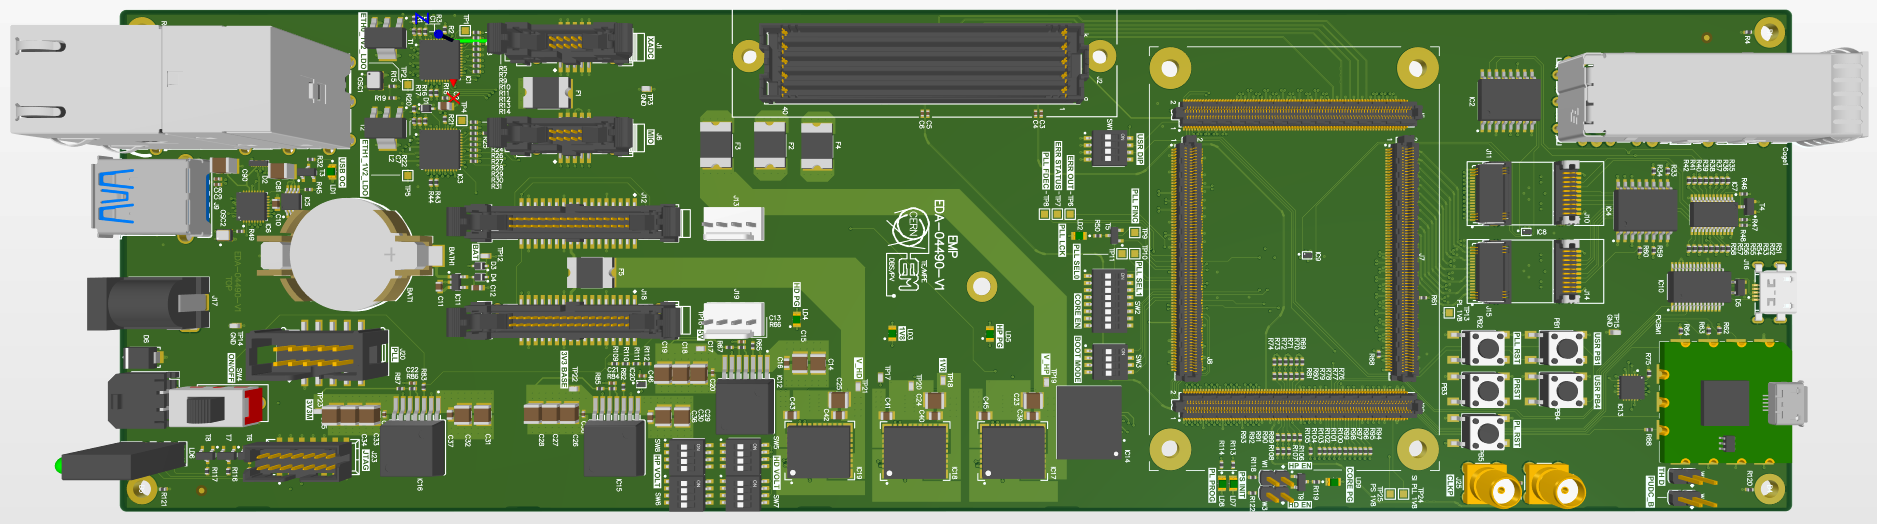
\includegraphics[width=1\textwidth]{Graphics/EMP_3d.PNG}
    \caption{3D top view of the EMP.}
    \label{fig:altiumEMP}
\end{figure}

\noindent One could manually confirm each pin by measurement, but this will be tedious with several pins on several boards. Instead, a test has been developed to ease this process.\\

\noindent For this test, the GPIO's are wired in a pin-to-pin configuration. The purpose of this configuration is that one GPIO can act as output, while simultaneously, the connected GPIO counterpart can act as an input. In this configuration, the output GPIO can be set to a value, and the input GPIO should be able to read it, and the other way around. If the input successfully reads the intended value, the GPIO can be confirmed to work.

As a result, the GPIO's can validate each other's ability to read or write. This will ease the validation without the need for a tedious process of examining all pins manually.

\subsection{Creating the firmware}

The firmware for the GPIO test is designed in VHDL using Vivado version 2020.1. At the time of writing, the EMP PCB board to be tested was still on its way. So for preparing firmware and software, a similar test is developed to represent the actual test. The only way this software and firmware differ from the actual test is for the pin headers used. \\

\noindent Nonetheless, this test deals with the same problems as the actual test and proves its behavior by quickly allowing manual measurement of pin headers. 

\subsubsection*{Create Vivado project}
Start Vivado, and create a new project by selecting File→Project→New. A pop-up window will appear with several project configuration options to go through when pressed. First, choose a fitting name and location for the application, and press 'Next'. For the project type, select 'RTL Project'. For the 'Add sources' and 'Add constraints' window, simply press next; the files will be added later. For the 'Default Part' page, the hardware used has to be specified. This must correlate to the Zynq used on the EMP. Search for the part named: xczu4eg-fbvb900-1-e. Press 'Next', and finally 'Finish' to create the project.

\subsubsection*{Create the Block Design}
Now that the project is created, click on 'Create Block Design' in the flow navigator. Again, choose a fitting name and press 'OK'. Now the modules used has to be added to the project. In this case, a module for the Zynq Processor and one for the GPIO. \\

\noindent To add the modules, open the diagram in the 'Flow Navigator' and press the plus sign '+' to add an IP (this can be done in several ways). When pressed, a pop-up window will appear. Here, search for the IP  named 'Zynq UltraScale+ MPSoC', and add the IP by double-pressing the name. 

To add the second module for the GPIO. Right-click on a blank space in the diagram, and click on 'Add IP...' in the drop-down menu. Here, search for the IP named: 
\mint{html}|AXI GPIO|
\noindent Again, double press to add the module. As a result, the block diagram should look like the one in figure \ref{fig:vivado_greenbar}. However, the placement of the modules makes no difference. 

\begin{figure}[H]
    \centering
    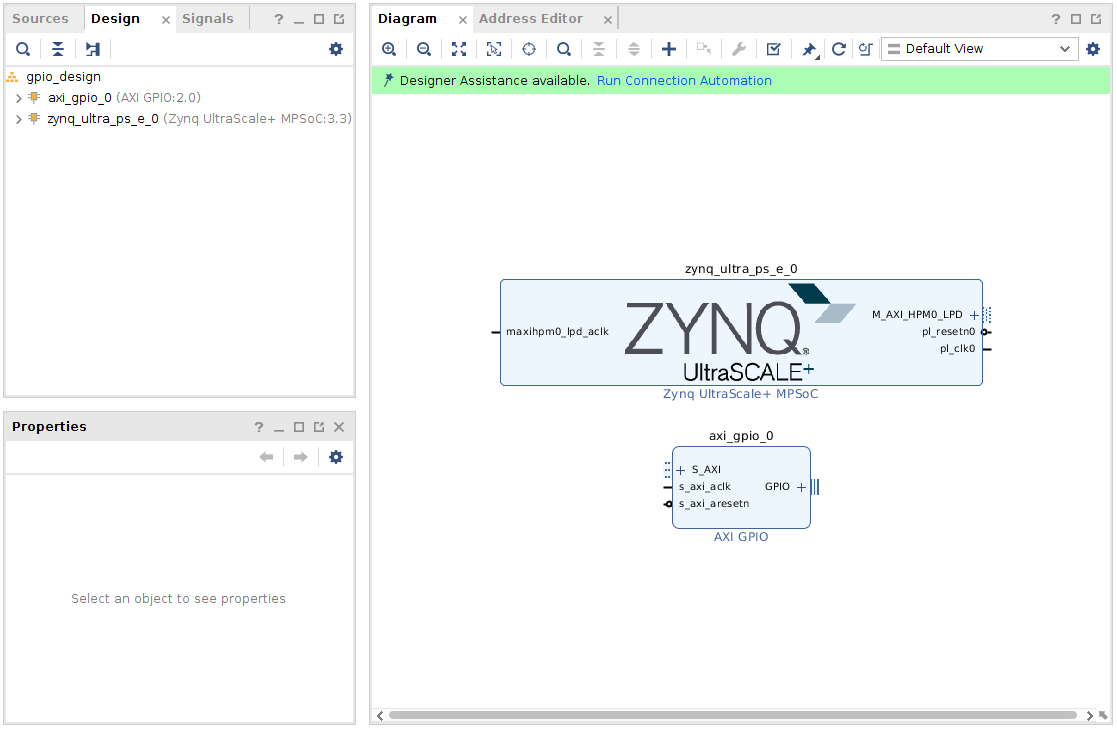
\includegraphics[width=1\textwidth]{Graphics/vivado_greenbar.PNG}
    \caption{3D top view of the EMP.}
    \label{fig:vivado_greenbar}
\end{figure}

\noindent When the two modules are added to the block design, a green bar should appear at the top of the window, with the text 'Designer Assistance available. Run 'Connection Automation', as shown on figure \ref{fig:vivado_greenbar}. Press it, and a pop-up window will now appear. Mark all boxes, and press 'OK'. Vivado automatically adds two new modules to the block diagram and attaches the necessary connections. Further, it created an external interface through the 'AXI GPIO'-module. This is shown in figure \ref{fig:vivado_auto}.

\begin{figure}[H]
    \centering
    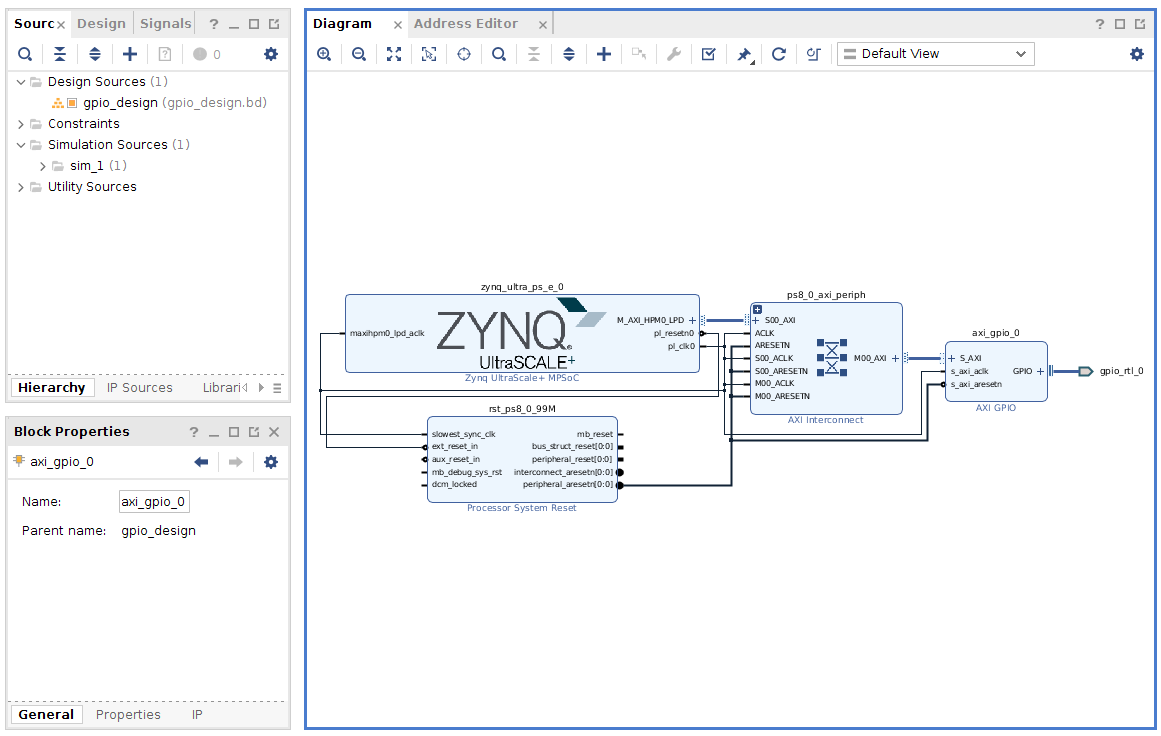
\includegraphics[width=1\textwidth]{Graphics/vivado_auto.PNG}
    \caption{3D top view of the EMP.}
    \label{fig:vivado_auto}
\end{figure}

\noindent Now double click on the 'AXI GPIO'-module to change the 'GPIO Width'; for this application, change it to 10, and press 'OK'. This defines the bit width of the GPIO channel and can be from 1 to 32. Where 32 is the default value. However, for now, 10 GPIO's lanes will do the job.

\subsubsection*{Xilinx Design Constraint (XDC) file}
Now the XDC (Xilinx Design Constraint) file needs to be written. The XDC file defines the requirements for the design in order to function on the board \cite{ug903viv24:online}. It essentially tells the software which physically pins on the FPGA there has to be utilized. Thus, before writing the XDC file, some research has to be done to locate these pins.\\

\noindent Since the Zynq Ultrascale+ TE0807 is placed on top of the TEBF0808 Trenz baseboard, it is necessary to look at the two components B2B (board-to-board) connections. This is to determine which pins to write in the XDC file to utilize the intended pin header on the EMP. 

For this, download the Pinout Planner excel file from Trenz's homepage named 'TE080x\_series\_pinout\_tracelength.xlsx' \cite{Download48:online}. In Excel, change the Carrier/Module combination to fit with the hardware. This is done by selecting 'TEBF0808\_REV04A' as the carrier and TE0807\_REV03 as the module. After updating, Excel now conforms to the hardware combination. Now, select the sheet named 'B2B Pin Table' in the sheet bar. \newline 

\noindent The FPGA Mezzanine Card, or FMC, present on the board is used. However, since measuring the value of a single FMC pinout is impractical, a Xilinx HW-FMC-105-DEBUG board is used. The Xilinx HW-FMC-105-DEBUG board allows better circumstances for manual measurements of each pin programmed, which will ease the job of confirming that it works. Nevertheless, unfortunately, this also introduces a bit more complexity, which will be explained later. The debugger board is shown in figure \ref{fig:EMP_with_debug} below.

\begin{figure}[H]
    \centering
    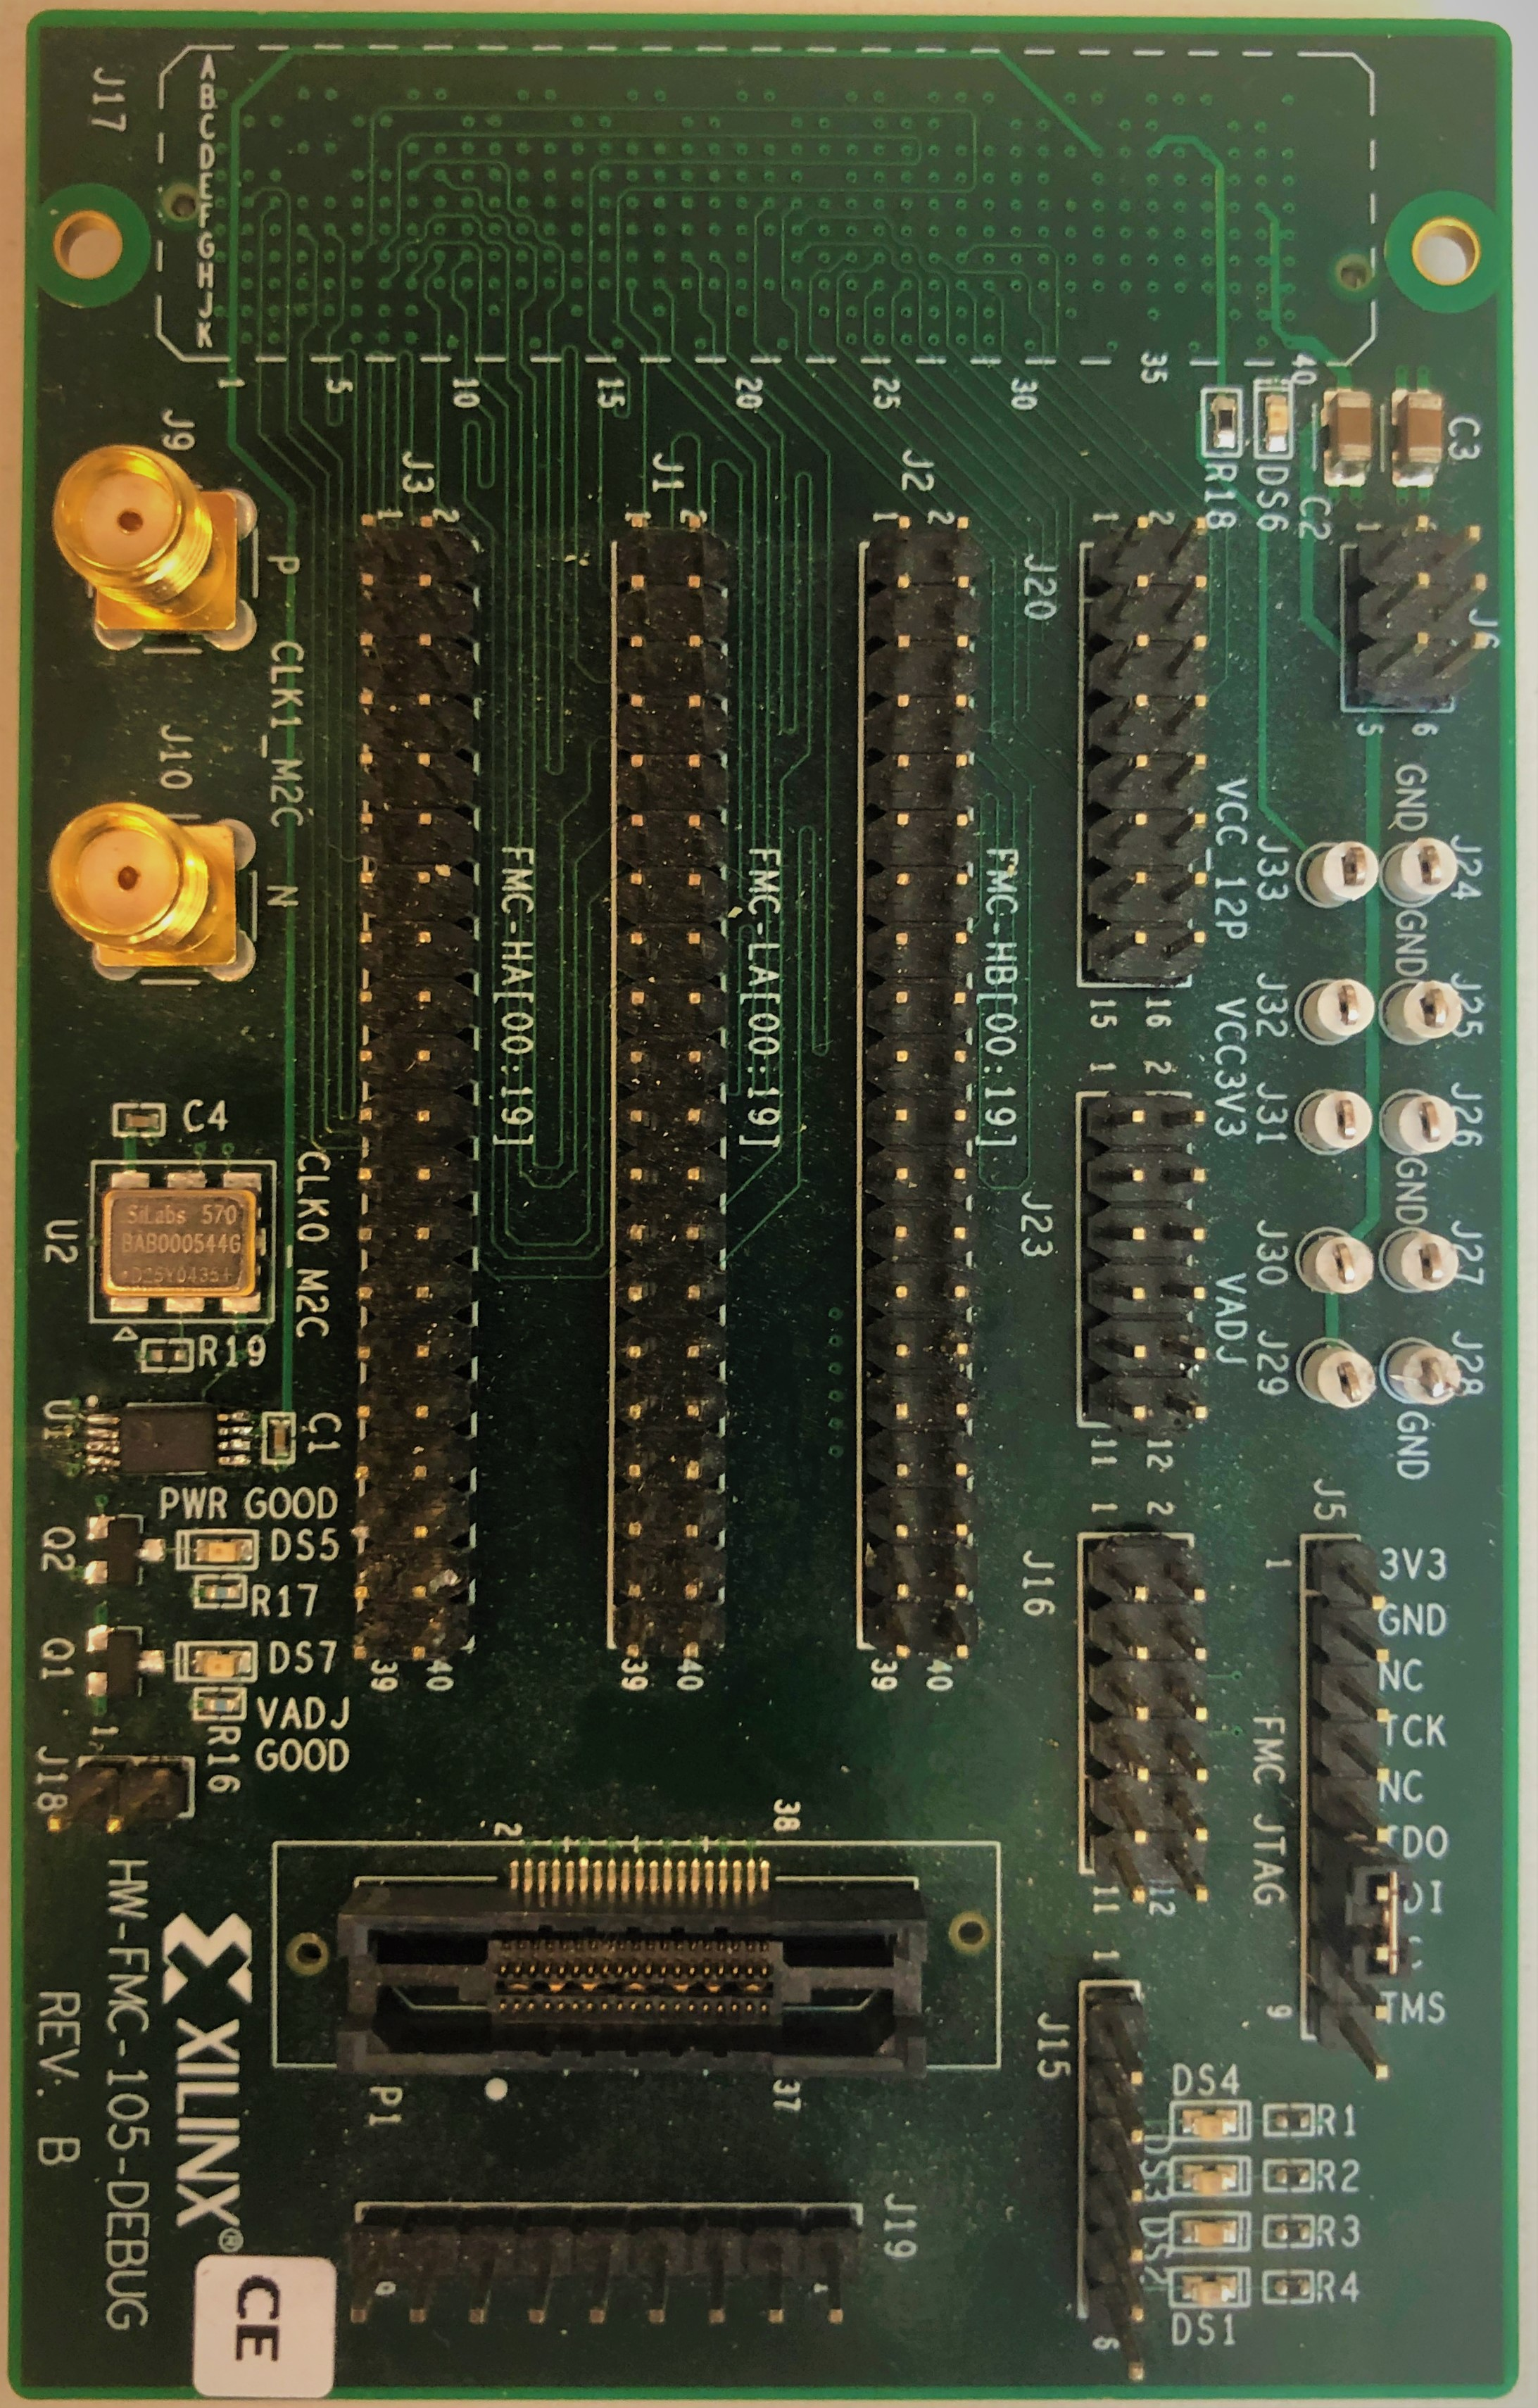
\includegraphics[width=.4\textwidth]{Graphics/FMC_top.jpg}
    \caption{Top view of the Xilinx HW-FMC-105-DEBUG board.}
    \label{fig:EMP_with_debug}
\end{figure}

\noindent And is mounted in the FMC present on the EMP, as shown in figure \ref{fig:EMP_with_debug}.

\begin{figure}[H]
    \centering
    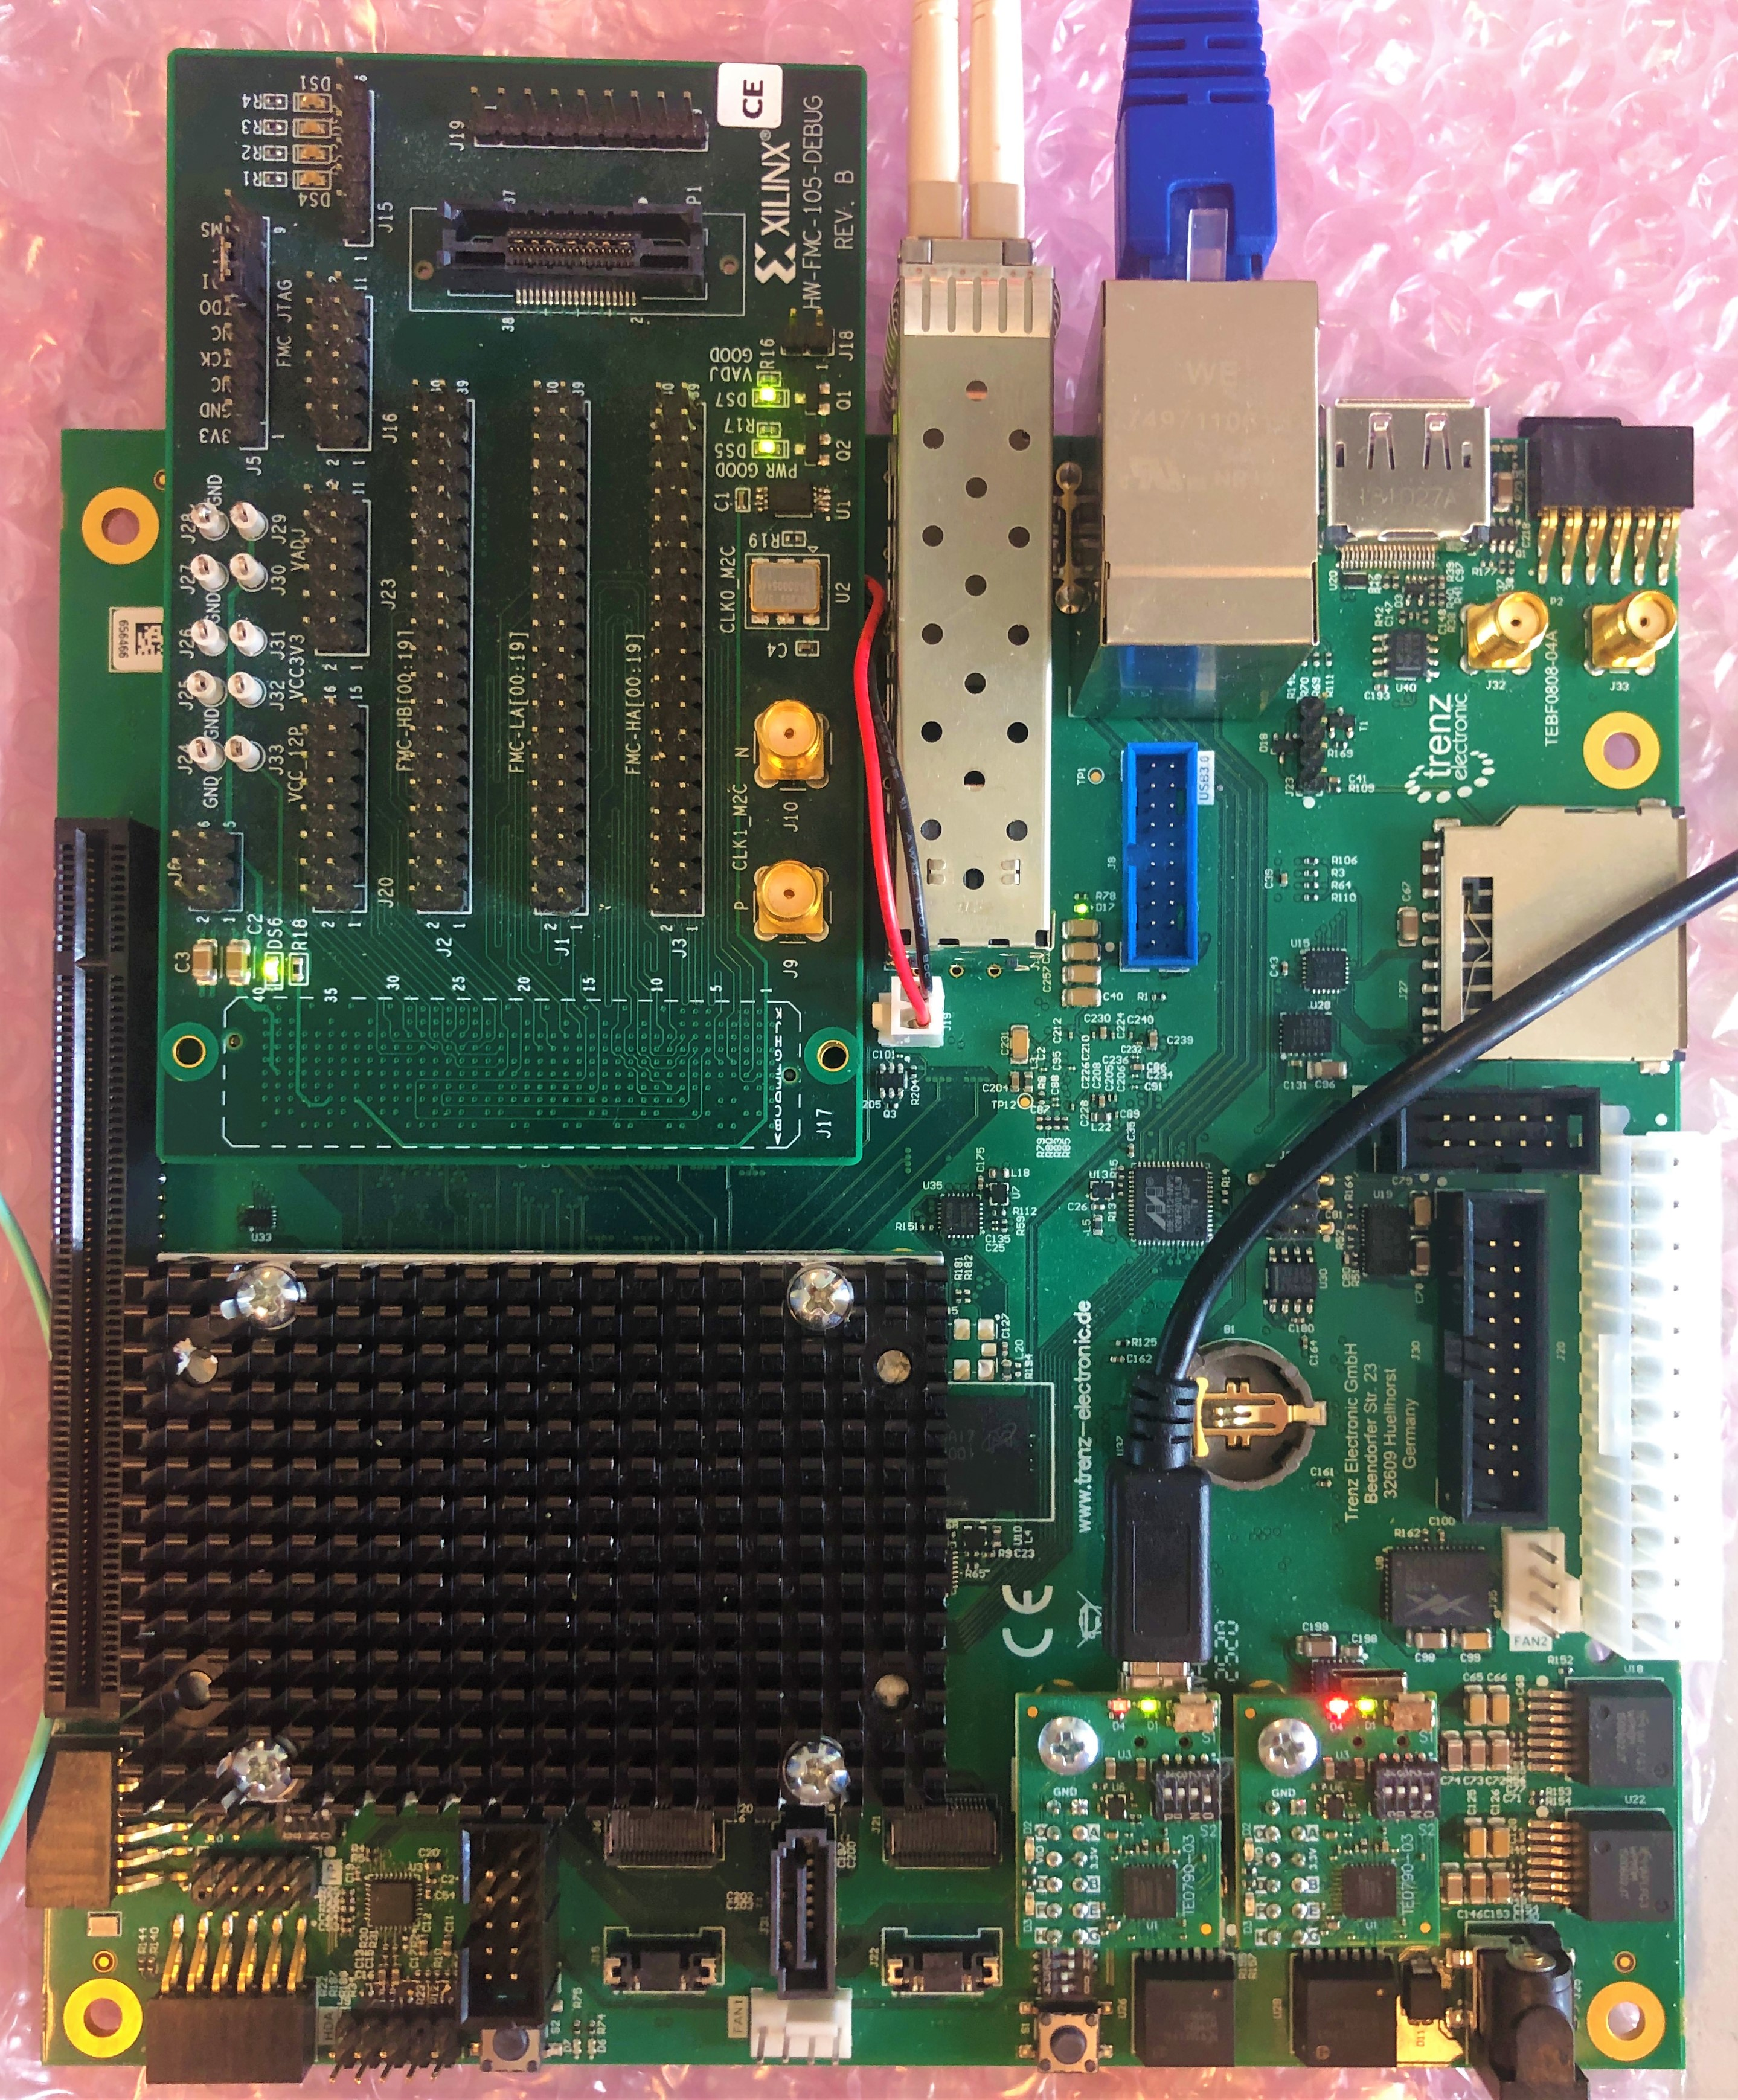
\includegraphics[width=.6\textwidth]{Graphics/EMP_with_debug.jpg}
    \caption{Top view of the EMP mounted with Xilinx debugger board.}
    \label{fig:EMP_with_debug}
\end{figure}

\noindent Now, the specific pins to be programmed can be selected. In this case, choosing the pins from 40 to 30 in connector J2 of the Xilinx debugger board is decided. Now, the correlation to the FPGA has to be determined.\\

\noindent From the datasheet of the Xilinx HW-FMC-105-DEBUG board \cite{ug537pdf71:online}, it is indicated which pins are connected to which FMC connector pins. E.g., in the case of using pin 40 in connector J2, the FMC pin E34 has to be programmed. As illustrated in the figure \ref{fig:FMC_pins} below, 

\begin{figure}[H]
    \centering
    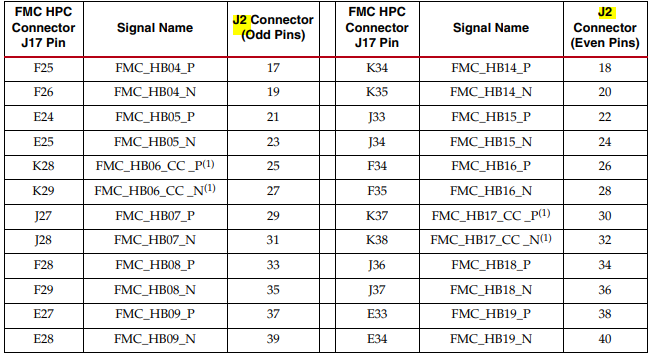
\includegraphics[width=1\textwidth]{Graphics/FMC_pins.PNG}
    \caption{ Table from FMC J17 to Connector J2 Pin Assignments.}
    \label{fig:FMC_pins}
\end{figure}

\noindent The FMC pin E34 denotes row E with column 34 in the connector and is also illustrated, with a red cross, in figure \ref{fig:FMC_figure} below. 

\begin{figure}[H]
    \centering
    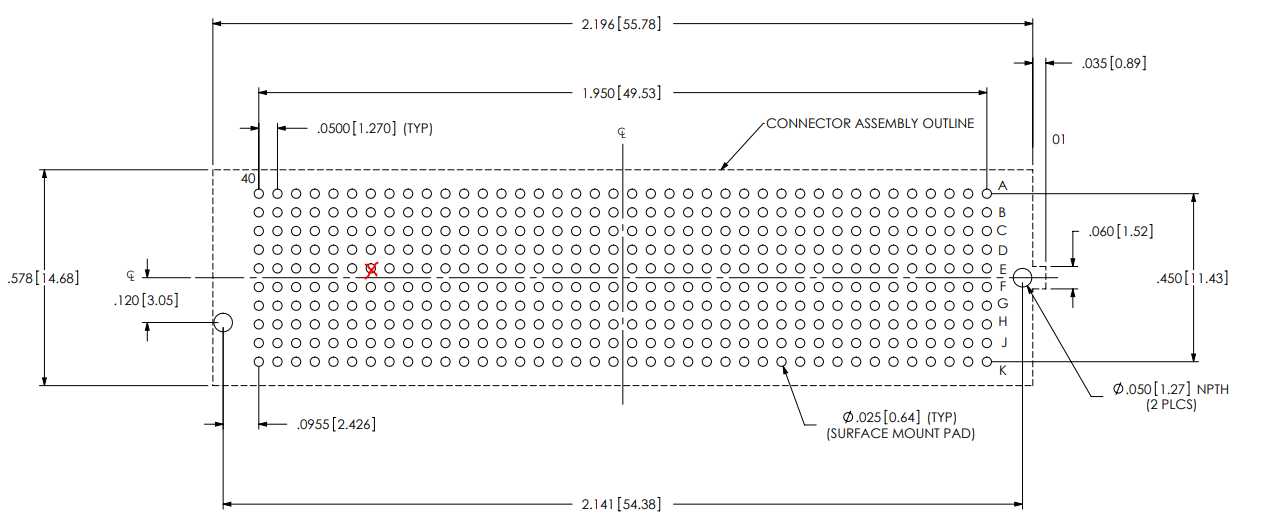
\includegraphics[width=1\textwidth]{Graphics/FMC_figure.PNG}
    \caption{Pin illustration of the ANSI/VITA 57.1 standard with E34 marked.}
    \label{fig:FMC_figure}
\end{figure}

\noindent With this knowledge, the Pinout Planner can be used. Search, or look for the value J5-E34. J5, because the FMC is B2B connector J5, and E34 because it is the pin desired to be used. When located, the information of the correlating FPGA pin K2 is shown. This is correspondingly illustrated in figure \ref{fig:pinout-planner}. 

\begin{figure}[H]
    \centering
    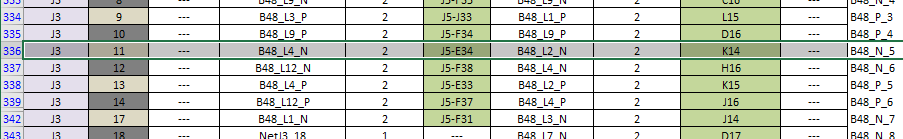
\includegraphics[width=1\textwidth]{Graphics/pinout-planner.PNG}
    \caption{Top view of the Xilinx HW-FMC-105-DEBUG board.}
    \label{fig:pinout-planner}
\end{figure}

\noindent The XDC file can now be created in Vivado. Click on 'Add Source' in the Flow Navigator, under the fold-down menu in the 'PROJECT MANAGER'. A pop-up window will now appear. Select 'Add or create constraint' and then 'Next'. Click 'Create File' and enter a file name that suits; in my case, I choose 'gpio\_io'. Create the file, and click 'Finish'. Now the constraint file will appear in the 'Sources'- tab. Open it, and then write the following code: 

\begin{listing}[H]
\begin{minted}[
        obeytabs=true,
        tabsize=1,
        numbersep=12pt,
        fontsize=\footnotesize]
        {VHDL}
set_property -dict {PACKAGE_PIN K14 IOSTANDARD LVCMOS18 } [get_ports gpio_rtl_0_tri_io[0]]
\end{minted}
\end{listing}
\vspace{-0.9 cm}
\noindent In the above code, the first command 'set\_property', is used to attach properties to the element. This is followed by the command '-dict', which is used to set a multiple properties in one line. This command is not mandatory, and the same code could still be written, but on two lines instead of one, like this:  
\begin{listing}[H]
\begin{minted}[
        obeytabs=true,
        tabsize=1,
        numbersep=12pt]
        {VHDL}
set_property PACKAGE_PIN K14 [get_ports gpio_rtl_0_io[0]]
set_property IOSTANDARD LVCMOS18 [get_ports gpio_rtl_0_tri_io[0]]
\end{minted}
\end{listing}
\vspace{-0.9 cm}
 \noindent The '-dict' command contains two additional properties: PACKAGE\_PIN and IOSTANDARD. PACKAGE\_PIN specifies which pin the signal should be assigned. In this example, it is the pin K14. IOSTANDARD, specify the voltage standard the pin should operate. In this case, the LVCMOS18 standard is used.
 
The last command [get\_ports gpio\_rtl\_0\_tri\_io[0]], tells Vivado to find the top-level port named gpio\_rtl\_0\_io[0], and connect the pins from '-dict' to the ports.

This procedure has to be done for all 10 pins used. This results in the XDC file \ref{code:xdc} below:
\begin{listing}[H]
\begin{minted}[
        obeytabs=true,
        tabsize=1,
        numbersep=12pt,
        fontsize=\footnotesize,
        highlightlines={},
        highlightcolor=newyellow]
        {VHDL}
#E34 - J2 pin 40
set_property -dict {PACKAGE_PIN K14 IOSTANDARD LVCMOS18} [get_ports{gpio_rtl_0_tri_io[0]}];
#E28 - J2 pin 39
set_property -dict {PACKAGE_PIN AG3 IOSTANDARD LVCMOS18} [get_ports{gpio_rtl_0_tri_io[1]}];
#E33 - J2 pin 38
set_property -dict {PACKAGE_PIN K15 IOSTANDARD LVCMOS18} [get_ports{gpio_rtl_0_tri_io[2]}];
#E27 - J2 pin 37
set_property -dict {PACKAGE_PIN AG4 IOSTANDARD LVCMOS18} [get_ports{gpio_rtl_0_tri_io[3]}];
#J37 - J2 pin 36
set_property -dict {PACKAGE_PIN A16 IOSTANDARD LVCMOS18} [get_ports{gpio_rtl_0_tri_io[4]}];
#F29 - J2 pin 35
set_property -dict {PACKAGE_PIN AH2 IOSTANDARD LVCMOS18} [get_ports{gpio_rtl_0_tri_io[5]}];
#J36 - J2 pin 34
set_property -dict {PACKAGE_PIN A17 IOSTANDARD LVCMOS18} [get_ports{gpio_rtl_0_tri_io[6]}];
#F28 - J2 pin 33
set_property -dict {PACKAGE_PIN AH3 IOSTANDARD LVCMOS18} [get_ports{gpio_rtl_0_tri_io[7]}];
#K38 - J2 pin 32 
set_property -dict {PACKAGE_PIN F15 IOSTANDARD LVCMOS18} [get_ports{gpio_rtl_0_tri_io[8]}];
#J28 - J2 pin 31
set_property -dict {PACKAGE_PIN AJ2 IOSTANDARD LVCMOS18} [get_ports{gpio_rtl_0_tri_io[9]}];

\end{minted}
\caption{Complete XDC file.}
\label{code:xdc}
\end{listing}

\noindent When the XDC file is created, click 'GENERATE BITSTREAM' in the 'FlowNavigator'. If the bitstream fails with the error [DRC NSTD-1], try to see chapter \ref{ch:[DRC nstd-1]} for help. If everything works, a successful bitstream is generated. Then, export the hardware by File→Export→Export Hardware. When the pop-up window appears, select 'Fixed' and press 'Next'. Select 'Include bitstream' and choose a name. For this project, 'gpio\_design\_wrapper' is used. Finally, finish by exporting it.

\subsubsection*{Preparing bitstream for programming} \label{sc:preparebitstream}
In this description, there is a considerable amount of information omitted. For a more in-depth understanding and walk-through, I highly recommend looking at chapter 8 of Morten's documentation \cite{document73:online},
or chapter 11 'How to use the EMP' of Daniel's Documentation \cite{FilesCER18:online}.\newline

\noindent The hardware exported now needs to be utilized on the EMP. To achieve this, a helpful script has been developed by Morten, named 'xsa-to-overlays' \cite{scripts·18:online}. Use it by entering the \textbf{/xsa-to-overlays} on the remote PC, and typing the command below, followed by the filename of the exported hardware from Vivado. Which in this case is:
\begin{figure}[H]
\begin{minted}[
        obeytabs=true,
        tabsize=1,
        numbersep=2pt]
        {bash}

$ ./emp-xsa-to-overlays.py gpio_design_wrapper.xsa

\end{minted}
\end{figure}
\vspace{-0.5 cm}
\noindent Press yes to the three following questions to complete, and now a .dbto and bit.bin file will appear in the \textbf{/output} folder. These files now needs to be moved to the \textbf{/lib/firmware} folder on the EMP. Which is done with the following command:

\begin{figure}[H]
\begin{minted}[
        obeytabs=true,
        tabsize=1,
        numbersep=2pt,
        fontsize=\small]
        {bash}

$ sudo mv ./gpio_design_wrapper.* /tftpboot/emp-01-00-02-centos8/lib/firmware/

\end{minted}
\end{figure}
\vspace{-0.4 cm}
\noindent Now, on the EMP, run the below command in the \textbf{/root} folder.

\begin{figure}[H]
\begin{minted}[
        obeytabs=true,
        tabsize=1,
        numbersep=2pt,
        fontsize=\small]
        {bash}

$ sudo ./petalinux-load-firmware.sh gpio_design_wrapper.dtbo

\end{minted}
\end{figure}
\vspace{-0.5 cm}
\noindent Now, the console will print the below warnings. This is just the default behavior when adding properties to a device tree node, and it will not impact the functionalities.\\
It is worth mentioning that the highlighted line below in figure \ref{Console_out} confirms that the GPIO hardware is registered at the address 0x80000000. This should be similar to the address seen in Vivado's 'Address Editor', as shown in figure \ref{fig:vivado_address} below.

\begin{figure}[H]
\begin{minted}[
        obeytabs=true,
        breaklines,
        tabsize=1,
        numbersep=2pt,
        fontsize=\scriptsize,
        highlightlines={13},
        highlightcolor=newyellow ] {bash}

[root@emp-trenz ~]$ sudo ./petalinux-load-firmware.sh gpio_design_wrapper.dtbo
mount: /configfs: configfs already mounted on /sys/kernel/config.
[ 2973.275899] fpga_manager fpga0: writing gpio_design_wrapper.bit.bin to Xilinx ZynqMP FPGA Manager
[ 2973.502881] OF: overlay: WARNING: memory leak will occur if overlay removed, property: /fpga-full/firmware-name
[ 2973.512965] OF: overlay: WARNING: memory leak will occur if overlay removed, property: /fpga-full/resets
[ 2973.522569] OF: overlay: WARNING: memory leak will occur if overlay removed, property: /__symbols__/overlay0
[ 2973.532403] OF: overlay: WARNING: memory leak will occur if overlay removed, property: /__symbols__/overlay1
[ 2973.542231] OF: overlay: WARNING: memory leak will occur if overlay removed, property: /__symbols__/afi0
[ 2973.551709] OF: overlay: WARNING: memory leak will occur if overlay removed, property: /__symbols__/clocking0
[ 2973.561622] OF: overlay: WARNING: memory leak will occur if overlay removed, property: /__symbols__/overlay2
[ 2973.571448] OF: overlay: WARNING: memory leak will occur if overlay removed, property: /__symbols__/axi_gpio_0
[ 2973.586767] GPIO IRQ not connected
[ 2973.590167] XGpio: gpio@80000000: registered, base is 328

\end{minted}
\vspace{-0.6 cm}
\caption{Console output when PL is generated.}\label{Console_out}
\end{figure}
\vspace{-0.4 cm}

\begin{figure}[H]
    \centering
    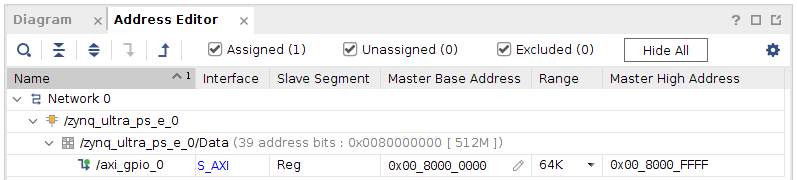
\includegraphics[width=1\textwidth]{Graphics/vivado_address.PNG}
    \caption{Screenshot from Vivado Address Editor.}
    \label{fig:vivado_address}
\end{figure}

\noindent Furthermore, it is shown that it has the base 328. What this means will be explained later.

\subsection{GPIO with Sysfs}

To access the GPIO hardware from a program, sysfs is used. Sysfs is a simple way to access a GPIO from userspace by making the device visible and accessible in the Linux file system. This also makes it easy to experiment with different configurations in the command line without coding. 

\subsubsection*{Find the right gpiochip} \label{gpiochip}

The GPIO hardware generated in the PL will be visible in \textbf{/sys/class/gpio}. When entering the folder, two gpiochips should be visible. 

\begin{figure}[H]
\begin{minted}[
        obeytabs=true,
        breaklines,
        tabsize=1,
        numbersep=2pt,
        fontsize=\small]
        {bash}

$ ls /sys/class/gpio/ #Shows gpiochips avaliable
>> export  gpiochip328  gpiochip338  unexport

\end{minted}
\end{figure}
\vspace{-0.6 cm}
\noindent

\noindent One of these gpiochips is the one exported from Vivado. To figure out which - inspect the number alongside the name. This number represents the base number of the GPIO, and from the console output of the PL generation \ref{Console_out}, it was shown that this base address was 328. Another way to find this information is by entering the gpiochip folder and printing the label, as shown below. 

\begin{figure}[H]
\begin{minted}[
        obeytabs=true,
        breaklines,
        tabsize=1,
        numbersep=2pt,
        fontsize=\small]
        {bash}

$ cd /sys/class/gpio/; ls
>> export  gpiochip328  gpiochip338  unexport
$ cat gpiochip328/label
>> /amba/gpio@80000000
$ cat gpiochip338/label
>> zynqmp_gpio

\end{minted}
\end{figure}
\vspace{-0.6 cm}

\noindent Here, the label gpio@80000000 of gpiochip328 matches the address from Vivado. In contrast is gpiochip338, not related to the Vivado module. However, instead of controlling the built-in GPIO's.

\subsubsection*{Export GPIO signals}

To use the GPIO's, the signals must first be exported into the sysfs. From Vivado it is known that the width of the GPIO was configured to 10. If in doubt, this can also be shown by:
\begin{figure}[H]
\begin{minted}[
        obeytabs=true,
        breaklines,
        tabsize=1,
        numbersep=2pt,
        fontsize=\small]
        {bash}
$ cat gpiochip328/ngpio
>> 10

\end{minted}
\end{figure}
\vspace{-0.6 cm}
\noindent This means that ten signals can be exported, beginning from 328 and ending at 337. 
The signal preferred must be written to the export file to export it. As shown below. 

\begin{figure}[H]
\begin{minted}[
        obeytabs=true,
        breaklines,
        tabsize=1,
        numbersep=2pt,
        %firstnumber=,
        fontsize=\small]
        {bash}
#Exports the GPIO signal 328. Corresponds to the 1. GPIO
$ echo 328 > /sys/class/gpio/export
$ ls
>> export  gpio328  gpiochip328  gpiochip338  unexport

#Exports the GPIO signal 329. Corresponds to the 2. GPIO
$ echo 329 > /sys/class/gpio/export 
>> export  gpio328  gpio329  gpiochip328  gpiochip338  unexport

\end{minted}
\end{figure}
\vspace{-0.6 cm}
\noindent
A new folder is created for each signal exported, and the GPIO is now accessible to the userspace. Inside the folder are different files with different GPIO signal options. For more information, see 'GPIO Sysfs Interface for Userspace' \cite{httpswww60:online}.

\begin{example}
To know which GPIO corresponds to which pin header, inspect the .XDC file in Vivado. Each element of the gpio\_rtl\_0\_tri\_io (starting from zero) corresponds to an element of the gpiochip328. Such that gpio\_rtl\_0\_tri\_io[0] correlate to gpio328. gpio\_rtl\_0\_tri\_io[1] to gpio329 and etc. 
\end{example}

\subsection{Programming of gpio\_test}
At this point, it is known how to manually control each GPIO exported from Vivado through sysfs. Now, this should be made into a C program for automatic testing of the interface on the EMP.\\
\noindent The aim of this program is mentioned at the beginning of the chapter. Nevertheless, a short resume is given below.

\vspace{-0.2 cm}
\paragraph{Resume of the desired program:} \hspace{-0.4 cm} \textit{
The GPIO’s should be wired in a pin-to-pin configuration, such that one GPIO can act as output while simultaneously, the connected GPIO counterpart can act as an input.
The output GPIO should now set a value, and the input GPIO should be able to read it. If the input successfully reads the intended value, the GPIO can be confirmed to work.
}\\

\noindent The code can be found \href{https://gitlab.cern.ch/esandgaa/gpio_test}{here}. 

\subsection*{Code description} 
The code uses strings to define the paths of where to open or write to each file. These files are the ones that configure the GPIO signal options, as mentioned above. Each GPIO is configured using a for loop, beginning from the first GPIO signal, defined in the .xdc file in Vivado, which was the FPGA pin K14 corresponding to the pin-header 40 on the debugger board.\\

\noindent In the for-loop, every GPIO signal is further divided into two equal-sized groups, decided by the order they appear in the for-loop. The group decides whether the GPIO signals should be an in- or output; if it is output, it sets the value to 0 (ground). 

\begin{example}
It will be rational to think that the GPIO output always should be set as high to allow the input GPIO input to perceive the signal. However, this is not true. The pins used for this application are LVDS, which, in short, implies that one of the pins is by default low while the other is default high. Therefore, some GPIO output signals need to be set low to be perceived at the input. 
\end{example}

\noindent When the for-loop is finished, each GPIO signal is configured as desired and ready to be validated. Hereafter, a new for-loop is created. Each run in this for-loop takes one GPIO signal from each group (i.e. one input and one output) and sets them as a pair. If the input corresponds to the output, it is successful.\\

\noindent Unfortunately, this is not enough to verify that this input is precisely the one from the GPIO counterpart. It could, for some reason, have been pulled down, or an incorrect pin-to-pin configuration could have done that.

So, to be sure, the same test is therefore repeated. However, this time, with the inverse configurations. So that the previous input now will be an output, and vice versa. This also means that the output value now will be high instead of low.\\

\noindent When both tests have been made, a final validation is made. Both of the above tests have to be successful to succeed in this. If not, an error in the GPIO is detected.\\
\noindent Below is a console output shown for the gpio\_test.

\begin{figure}[H]
\begin{minted}[
        frame=single,
        obeytabs=true,
        breaklines,
        tabsize=1,
        numbersep=2pt,
        %firstnumber=,
        fontsize=\small]
        {bash}
$ /gpio_test/gpio_test 328
 GPIO test
***************************************************************************
 Test:     Pins:        Output:  Input:         Status:
***************************************************************************
 Test1: (40 --> 39)       0        1            Failed
 Test2: (38 --> 37)       0        0            Success
 Test3: (36 --> 35)       0        1            Failed
 Test4: (34 --> 33)       0        1            Failed
 Test5: (32 --> 31)       0        1            Failed
***************************************************************************
 Switching input and output
***************************************************************************
 Test6: (39 --> 40)       1        0            Failed
 Test7: (37 --> 38)       1        1            Success
 Test8: (35 --> 36)       1        0            Failed
 Test9: (33 --> 34)       1        0            Failed
 Test10: (31 --> 32)      1        0            Failed
***************************************************************************
 Final Test Result
***************************************************************************
 Test between (40 <--> 39)                      Failed
 Test between (38 <--> 37)                      Success
 Test between (36 <--> 35)                      Failed
 Test between (34 <--> 33)                      Failed
 Test between (32 <--> 31)                      Failed
***************************************************************************
Number of errors are: 4

\end{minted}
\vspace{-0.6 cm}
\caption{Console output of gpio\_test.}
\end{figure}
\vspace{-0.2 cm}
\noindent

\noindent A pin-to-pin configuration is only created between pin-header 38 and 37, as shown in the picture below.

\begin{figure}[H]
    \centering
    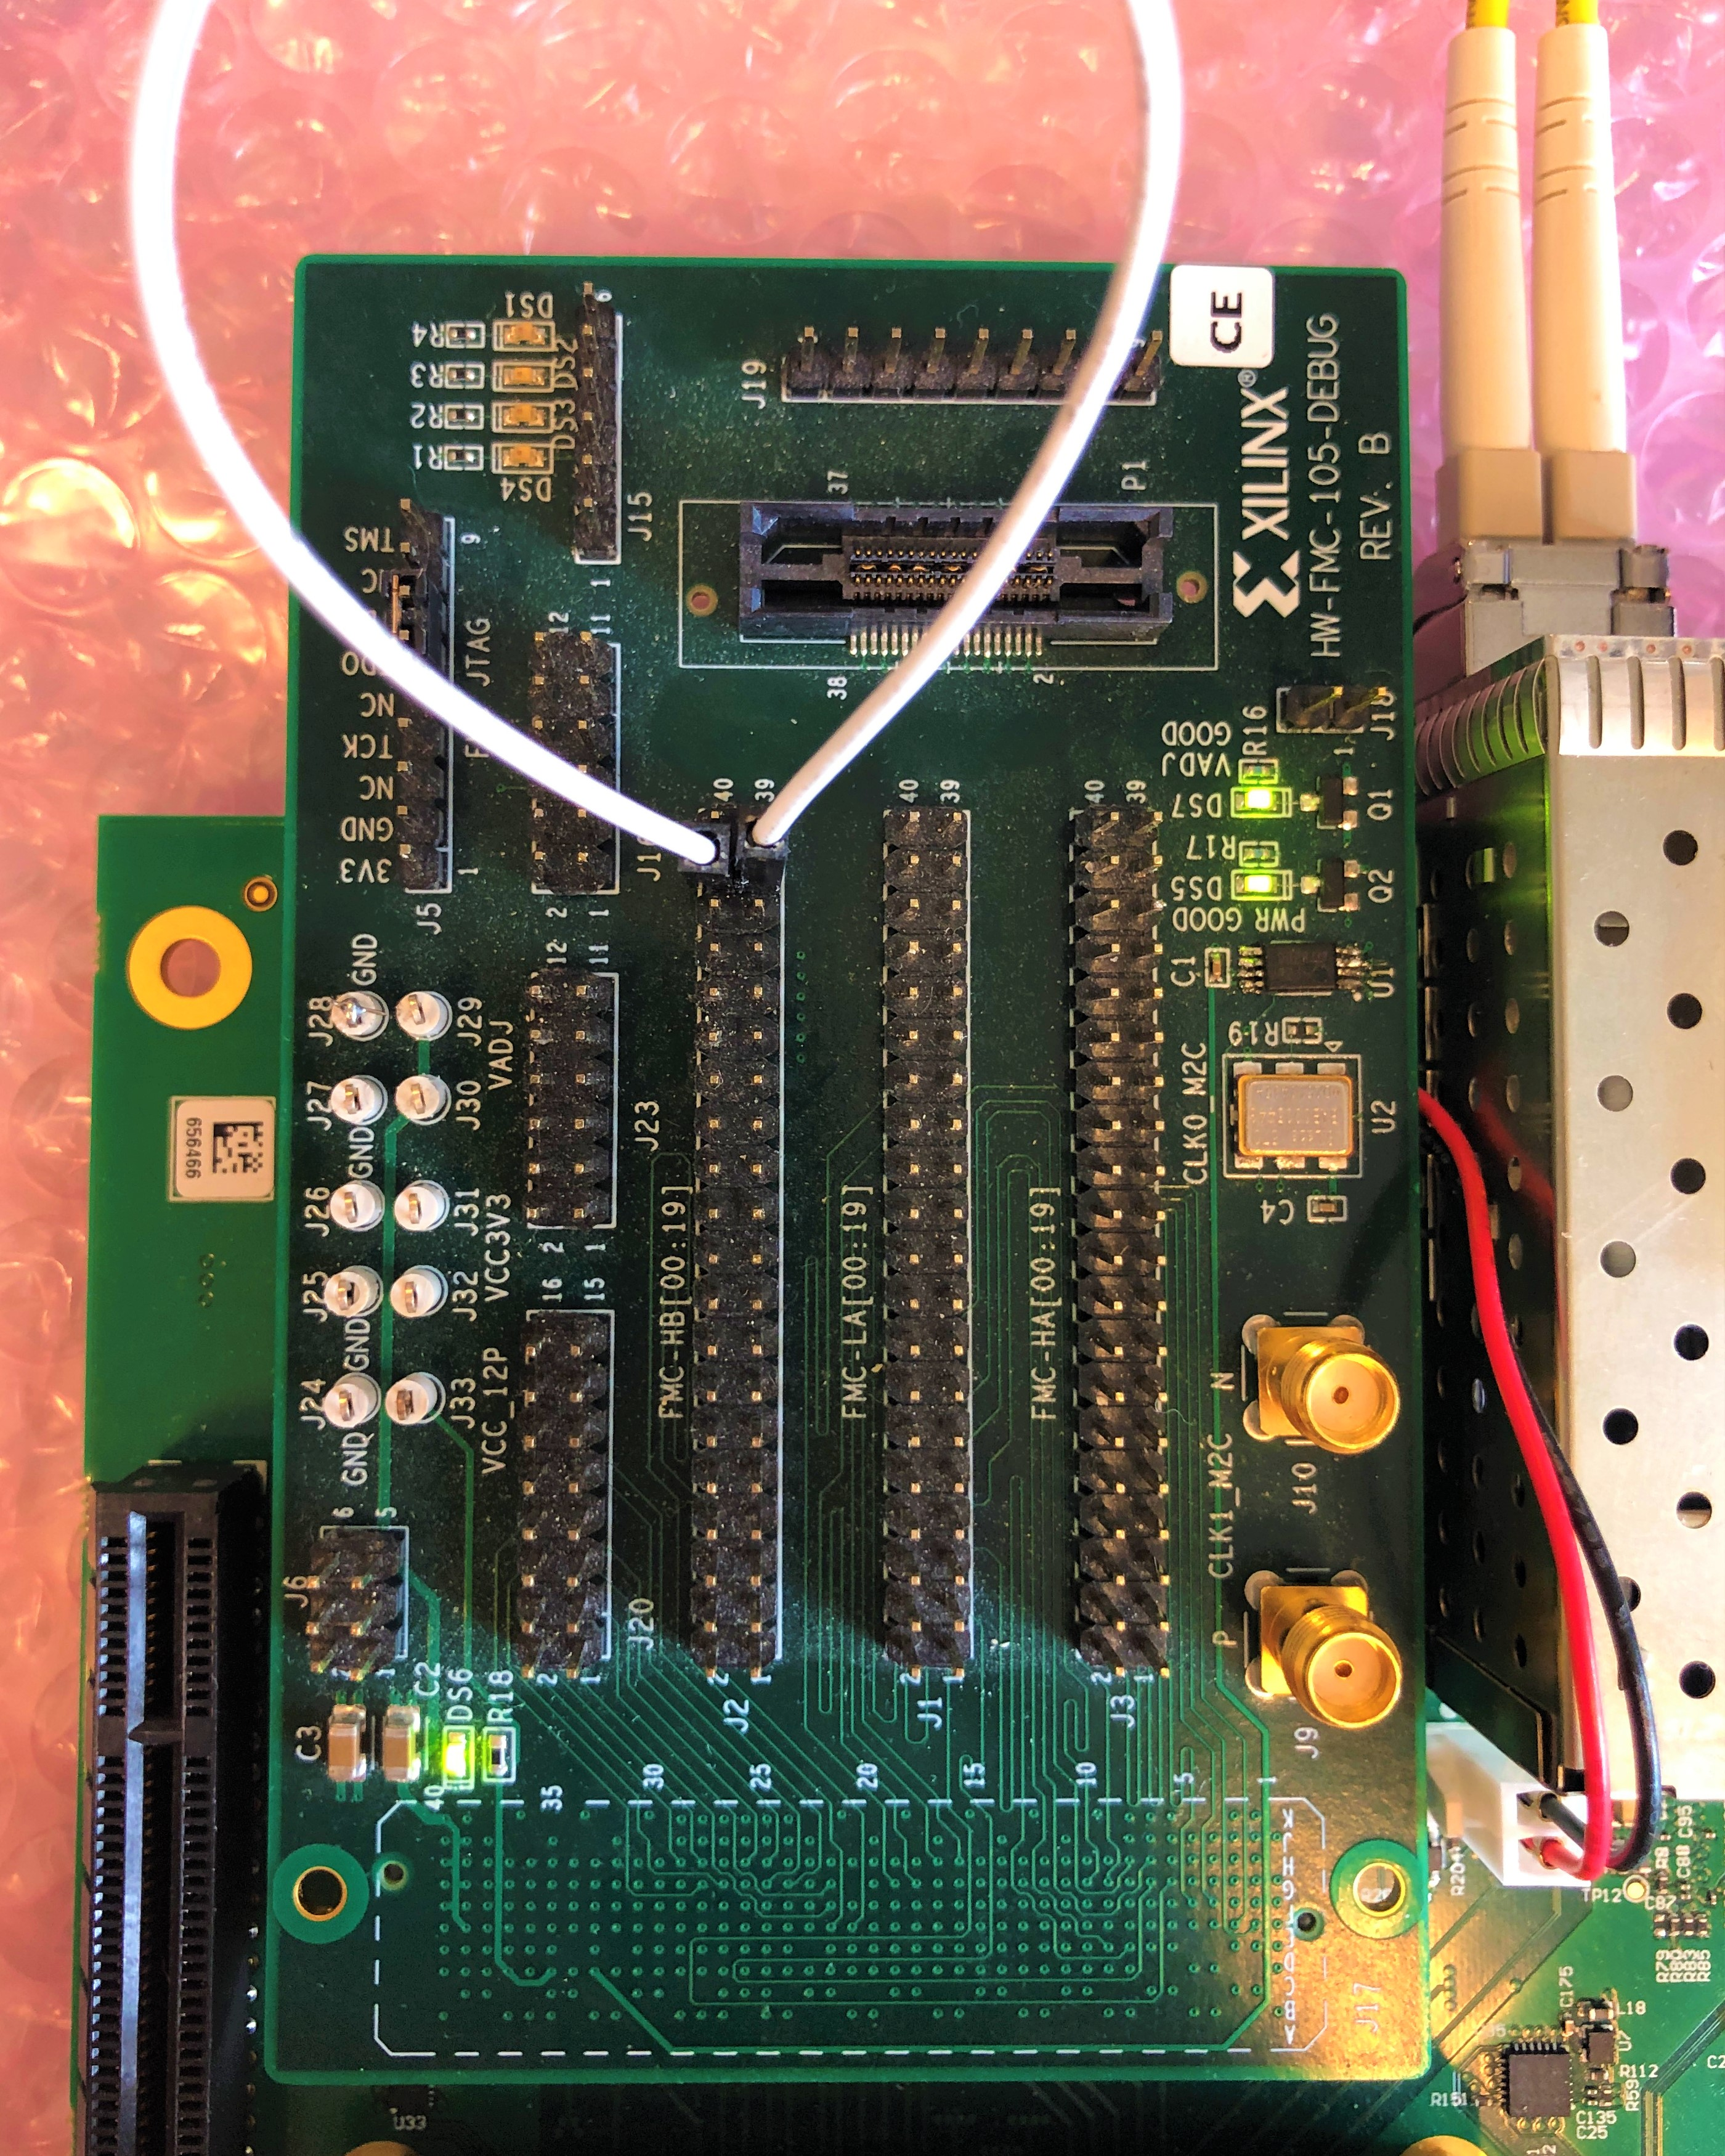
\includegraphics[width=.6\textwidth]{Graphics/pintopin.jpg}
    \caption{Picture with the a pin-to-pin configuration between pin-header 38 and 37.}
    \label{fig:vivado_address}
\end{figure}

\subsection{Usage of gpio\_test}

To use the gpio\_test, pass an argument with the value of the base number, as shown below. 

\begin{figure}[H]
\begin{minted}[
        obeytabs=true,
        breaklines,
        tabsize=1,
        numbersep=2pt,
        %firstnumber=,
        fontsize=\small]
        {bash}
/gpio_test/gpio_test <base number>

\end{minted}
\end{figure}
\vspace{-0.9 cm}
\noindent The base address can be found as explained in \ref{gpiochip}.

\subsection{Limitations of the gpio\_test}
The code is limited in its flexibility as it makes some significant assumptions.\\

\noindent Each GPIO signal in the code corresponds to a pin port defined in the .XDC file in Vivado, and there is no way to tell if these pins still correlate if the .XDC file is changed. The code is built to fit the Vivado project; if that changes, the program has to be changed. 

\vspace{-0.3 cm}
\paragraph{Assumptions:}
\begin{enumerate}
\vspace{-0.1 cm}
    \item The first and highest pin-header is 40
    \vspace{-0.3 cm}
    \item Every pin number followed are declined by 1.  
    \vspace{-0.3 cm}
    \item The pin-to-pin are configured between two subsequent GPIO signals. Such that GPIO 40 \& 39 is a pair, GPIO 38 \& 37 is a pair and ect.  
\end{enumerate}

\noindent If any of the above assumptions are changed, the code must be modified.

\subsection*{Recommendations if modifying the .xdc file}

\noindent When changing the .xdc file in Vivado, it is recommended to sort the pin in the desired pin-to-pin pairs.  

\begin{listing}[H]
\begin{minted}[
        obeytabs=true,
        tabsize=1,
        numbersep=12pt,
        fontsize=\footnotesize,
        highlightlines={2, 4},
        highlightcolor=newyellow]
        {VHDL}
#E34 - J2 pin 40
set_property -dict {PACKAGE_PIN K14 IOSTANDARD LVCMOS18} [get_ports{gpio_rtl_0_tri_io[0]}];
#E28 - J2 pin 39
set_property -dict {PACKAGE_PIN AG3 IOSTANDARD LVCMOS18} [get_ports{gpio_rtl_0_tri_io[1]}];
#E33 - J2 pin 38
set_property -dict {PACKAGE_PIN K15 IOSTANDARD LVCMOS18} [get_ports{gpio_rtl_0_tri_io[2]}];
#E27 - J2 pin 37
 ...
\end{minted}
\vspace{-0.5 cm}
\caption{Highlighted pin-to-pin pair in .xdc file.}
\label{code:xdc}
\vspace{-0.3 cm}
\end{listing}
\noindent In the above code the pin-header 40 (corresponds to FPGA pin K14) and pin-header 39 (corresponds to FPGA pin AG3) is desired to be linked in a pin-to-pin configuration. Hence, it is sorted to be next to each ([get\_ports{gpio\_rtl\_0\_tri\_io[0]}] and [get\_ports{gpio\_rtl\_0\_tri\_io[1]}]). 

\subsection{Conclusion}

The code makes an excellent foundation for a later test of the GPIO interface. Unfortunately, the assumptions made in the code make the program very limited in flexibility. As a result, it is recommended to adopt this code for each GPIO test desired.


\chapter{Analysis of internship}

In this chapter, I will go through the gain acquired during the internship within the below fields:

\begin{itemize}
    \item Academic
    \item Work-related
    \item Social
\end{itemize}

\noindent These three subjects will cover my overall experience and knowledge from working at CERN.

\section{Academic}

In terms of academic knowledge, there are significant opportunities for gaining knowledge at CERN. CERN provides a library for all its employees with several books covering a lot of the fields within programming, field theory, particles, magnetism, etc. Furthermore, several times weekly, CERN hosts seminars for its employees. Though, some of these seminars can be very specialized and hard to follow if you are not already in the field of the subject. There are also seminars hosted to give a more superficial knowledge of the field. Attending these seminars is free and is optional. \\

\noindent During my time at CERN, I attended three seminars. Here among one from DeepMind. DeepMind is a company within the field of A.I., and they wanted to give insight into their results and further explain how this technology could be used for the detectors at CERN. It was fascinating to follow and inspired me to attain more knowledge in the field or maybe to continue studying in the field of Artificial intelligence one day. 
Besides that, I was attending a seminar about privacy in the world of tomorrow. These seminars are just examples of a large amount of seminars offered during my time at CERN. \\

\section{Work related}

While working at CERN, I learned a lot. I felt so fortunate with the projects assigned to me. The projects allowed me to work and gain knowledge within many different aspects in the field of electronics. In that way, I can tell what I find the most interesting for me to work with at a later point in life. I had the opportunity to create the firmware and the associated software. Working in a computer's different  "layers" was a perfect way ´for "connect the dots" learned at the university. 

\section{Social}

Besides restrictions due to Covid during the first two months of the internship, there were great opportunities at CERN for socializing. For example, CERN has many clubs that could be joined based on one's interests. These clubs include football, chess, basketball, skiing, etc.\\

\noindent Besides the clubs, newcomers arriving at CERN are being brought together with a meeting and added to a shared chat group. In these chat groups, people are amiable and often invite group members to hang out in their spare time.  \\

\noindent At CERN, there is also a particular group for only danish interns. This group is for all the newcomers who arrived at CERN and is brought together by Jørgen. I will shortly mention Jørgen here, as he has a significant impact on the way danish interns are socializing at CERN. \\

\noindent Jørgen has been working at CERN for more than 30 years.
Besides his work, he is doing a lot of work to give the danish interns the best prerequisites for their stay. He is not only arranging social gatherings but is also our person to contact in case of any trouble regarding our stay at CERN. He has even rented his car to an intern so that he could manage some paperwork for his residential conditions. \\

\noindent During my time, I also improved my social skills and language. It was necessary, as I had to make new friends and get along with my roommate and colleagues. Here I had no trouble socializing, even though Covid made it hard. Often I arranged social gatherings, either in the town of Geneva for a beer or at my place for dinner. Every Friday, we even made a beer tradition. So even though people might have been busy on workdays, there was this point every week to catch up. 

% \section{Knowledge exchange}

% Frankly, there was not a lot of knowledge exchange from AAU to CERN. The knowledge I had gained at the university was not new to CERN. In some way, it was a bit old. An example of this is one of the tools used at the university, Xilinx ISE, which is starting to be phased out. Today, the new tool is "Vivado". It was a bit pitty to find out some of the knowledge acquired at the university already was old. But I understand that the growth of the technologies in this field is evolving so fast that it might be hard for the universities to keep up with the pace.

\section{Obtained experience}

\noindent During my time at CERN, I gained many experiences I would benefit from in the future. Among them stand the experience of getting knowledge about the differences between peoples across cultures in the workspace. I see this experience as a significant trait as I may, in the future, work in corporations with employees from numerous nations. Other than that, I have been more motivated and experienced in future opportunities of working abroad. This is not only on a professional level but also on a personal level. Retaining to new and foreign environments is crucial when working abroad. Furthermore, getting more experience in English was excellent as many jobs require fluent English.\\

\noindent Work related I got to experience the "real world". I learned how to utilize my knowledge gained from the university into something useful for CERN to meet the desired outcome. Furthermore, as Aalborg university presupposes a lot of group work, it was nice to have the experience of full responsibility and development for the work accomplished.

\chapter{Conclusion}

Overall I am very grateful that I was given a chance to work at CERN. I was very satisfied with my project, as it allowed me to learn many aspects of embedded software. Furthermore, it also allowed me to work within different areas in the field and to get a sensation of what I will find most enjoyable to work with in the future.\\

\noindent I spent most of my time acquiring new knowledge for the project for afterward applying it. That meant that the learning curve during my time was very steep. Furthermore, working on the project has given me a more in-depth understanding of the theory learned in the courses at the university. \\

\noindent Working at CERN has given me insight into the profession. Working in a small development team within a large organization has given me an understanding of how the development of a product takes place. It has given me insight into the collaboration across groups, the responsibilities, and deadlines.\\

\noindent Being an intern at CERN has given me a lot of great experiences. To walk around and witness the outstanding creations of the LHC and anti-matter factory inspires and is highly motivating. It reminds me of the remarkable achievements in science and our unimaginable universe. \\

\noindent Furthermore, living abroad gives a meaningful personal development. It provides a lot of insight into different cultures and diverse ways of thinking. Also, it reminds me of how lucky we should be in Denmark for our healthcare, financial situation, and working hours. Sadly, not many countries are as fortunate as we are. \\

\noindent This internship has made a tremendous impact on both a professional and personal level, and if I get the chance to work abroad again, I would definitely consider it.




















% If you do not write the report in English, translating the bibliography title to, e.g., Danish, should not be done here. Instead, you should change the main language in the preamble (look for the line \usepackage[danish,english]{babel} and change the order/delete the 'english' option). See more in the babel package documentation.
\printbibliography[heading=bibintoc, title=Bibliography]
\label{bib:mybiblio}
\appendix
\chapter{Diary}\label{ch:appDiary}
\section*{Genral work related information} \newline
 Working hours 8:30 - 17:30 Monday to Friday.
\section*{Daily worktasks}
\begin{description}
\item[(17/01)] First day at CERN. Introduced to my new colleagues and project.
\item[(18/01)] Introduction to the software tools and enviorments used.  
\item[(19/01)] Setup enviorments for developing. 
\item[(20/01)] Going through the manual by Morten, and looked into cross compiling.
\item[(21/01)] Researching PetaLinux, and started using VIM for developing C programs. First 'Hello world' on the EMP.
\item[(22/01)] Weekend.
\item[(23/01)] Weekend.
\item[(24/01)] Day off for taking the online project exam.
\item[(25/01)] Introduced to the NFS filesystem.
\item[(26/01)] Looking into developed code for communcation with the EMCI, which reads and writes registers of the lpGBT.
\item[(27/01)] Learning of Makefiles. Beginning developing of a cpp program to enable the clock generator present on the EMP. 
\item[(28/01)] Continuing working with the program. 
\item[(29/01)] Weekend
\item[(30/01)] Weekend
\item[(31/01)] Debugging the program with help from Daniel. 
\item[(1/02)] Continuing debugging and working on the code
\item[(2/02)] Learning about the I2C switch present on the board. 
\item[(3/02)] Getting into AirHDL. Further understanding for lpGBT, registers, AXI and I2C 
\item[(4/02)] Remote PC stopped working. Begining a new task of devoloping a GUI in python.
\item[(5/02)] Weekend
\item[(6/02)] Weekend
\item[(7/02)] Looking into Python
\item[(8/02)] Python excercise - Develope a GUI in .py which use a function from a .cpp file. 
\item[(9/02)] Excersise finished. Researching a solution for communication between the remote PC and the EMP, in such way that the remote PC proccessing the GUI.
\item[(10/02)] Further reasearching, and coding for test different approaches. 
\item[(11/02)] Looked further into an API. Including how bindings in .py (marshalling) works, Sockets, researching of what a IPC is, an the RESTful API architecture.  
\item[(12/02)] Weekend
\item[(13/02)] Weekend
\item[(14/02)] Beginning the 'Docker-getting-started' exercise
\item[(15/02)] Finished 'Docker-getting-started', dived further into docker by following some certification tasks and questions.
\item[(16/02)] Read Specifications documents regarding the EMP and further reading of Mortens manual
\item[(17/02)] Remote PC working again. Starting developing code for EMP.
\item[(18/02)] Looking further into how to connect the GUI with the EMP. Succesfully etablished a connection via a TCP socket between a .py and a .cpp code on two different devices.  
\item[(19/02)] Weekend
\item[(20/02)] Weekend
\item[(21/02)] Implemented multi thredding in code to trying to acomplish full duplex communicaton between server/client.
\item[(22/02)] Further working on implementing multi threadding in code, and made it succesfully. The server/client can now send and recieve at the same time.  
\item[(23/02)] Preparing Daniel's leaving at CERN. In this regard I looked further into communication between the EMP and the EMCI. Furthermore, trying to establish a broad understanding of the elements involved in the project, but with a deep understanding within my fiels of work. In such way, that I, with the help from Vladimir can continue the project, in a painless way. Hopefully any questions that might be relevant for this project in the future, will at this time be asked.  
\item[(24/02)] Looked into bit-banging, and the emp-intr code. 
\item[(25/02)] Meeting today for the ATLAS DCS front-end (EMCI - Embedded Monitoring and Control Interface) and back-end (EMP - Embedded Monitoring Processor).
\item[(26/02)] Weekend
\item[(27/02)] Weekend
\item[(28/02)] Problems with the clock. Trying to debug, and asking Daniel for help.
\item[(29/02)] 
\item[(01/03)] 
\item[(02/03)] 
\item[(03/03)] 
\item[(04/03)] 
\item[(05/03)] 
\item[(06/03)] 
\item[(07/03)] 
\item[(08/03)] 
\item[(09/03)] 
\item[(10/03)] Clock configuration finally works! Found the issue, which was cause by writing/reading 16-bit instead of 8-bit.
\item[(11/03)] 

\end{description}
\end{document}
